\documentclass{article}

\usepackage{arxiv}

\usepackage[utf8]{inputenc} % allow utf-8 input
\usepackage[T1]{fontenc}    % use 8-bit T1 fonts
\usepackage{lmodern}        % https://github.com/rstudio/rticles/issues/343
\usepackage{hyperref}       % hyperlinks
\usepackage{url}            % simple URL typesetting
\usepackage{booktabs}       % professional-quality tables
\usepackage{amsfonts}       % blackboard math symbols
\usepackage{nicefrac}       % compact symbols for 1/2, etc.
\usepackage{microtype}      % microtypography
\usepackage{graphicx}

\title{Unveiling Color Dynamics in Andy Warhol's ``Shot Marilyns'': A
Study on Visual Variations and Perception}

\author{
    Erick S. Arenas V
   \\
    Department of Statistics \\
    University of California, Davis \\
  Davis, CA 95616 \\
  \texttt{\href{mailto:esarenas@ucdavis.edu}{\nolinkurl{esarenas@ucdavis.edu}}} \\
   \And
    Weilin Cheng
   \\
    Department of Statistics \\
    University of California, Davis \\
  Davis, CA 95616 \\
  \texttt{\href{mailto:wncheng@ucdavis.edu}{\nolinkurl{wncheng@ucdavis.edu}}} \\
   \And
    Hengyuan Liu
   \\
    Department of Statistics \\
    University of California, Los Angeles \\
  Los Angeles, CA 90095 \\
  \texttt{\href{mailto:hengyuanliu@g.ucla.edu}{\nolinkurl{hengyuanliu@g.ucla.edu}}} \\
   \And
    Xinhui Luo
   \\
    Department of Statistics \\
    Tufts University \\
  Boston, MA 02155 \\
  \texttt{\href{mailto:xinhui.luo@tufts.edu}{\nolinkurl{xinhui.luo@tufts.edu}}} \\
   \And
    Kathy Mo
   \\
    Department of Statistics \\
    University of California, Los Angeles \\
  Los Angeles, CA 90095 \\
  \texttt{\href{mailto:kathymo24@g.ucla.edu}{\nolinkurl{kathymo24@g.ucla.edu}}} \\
   \And
    Li Yuan
   \\
    Department of Computer Science \\
    Swiss Federal Institute of Technology, Zurich \\
  8092 Zurich, Switzerland \\
  \texttt{\href{mailto:xxxx@ethz.ch}{\nolinkurl{xxxx@ethz.ch}}} \\
  }


% tightlist command for lists without linebreak
\providecommand{\tightlist}{%
  \setlength{\itemsep}{0pt}\setlength{\parskip}{0pt}}


% Pandoc citation processing
\newlength{\cslhangindent}
\setlength{\cslhangindent}{1.5em}
\newlength{\csllabelwidth}
\setlength{\csllabelwidth}{3em}
\newlength{\cslentryspacingunit} % times entry-spacing
\setlength{\cslentryspacingunit}{\parskip}
% for Pandoc 2.8 to 2.10.1
\newenvironment{cslreferences}%
  {}%
  {\par}
% For Pandoc 2.11+
\newenvironment{CSLReferences}[2] % #1 hanging-ident, #2 entry spacing
 {% don't indent paragraphs
  \setlength{\parindent}{0pt}
  % turn on hanging indent if param 1 is 1
  \ifodd #1
  \let\oldpar\par
  \def\par{\hangindent=\cslhangindent\oldpar}
  \fi
  % set entry spacing
  \setlength{\parskip}{#2\cslentryspacingunit}
 }%
 {}
\usepackage{calc}
\newcommand{\CSLBlock}[1]{#1\hfill\break}
\newcommand{\CSLLeftMargin}[1]{\parbox[t]{\csllabelwidth}{#1}}
\newcommand{\CSLRightInline}[1]{\parbox[t]{\linewidth - \csllabelwidth}{#1}\break}
\newcommand{\CSLIndent}[1]{\hspace{\cslhangindent}#1}

\usepackage{amsmath}
\usepackage{graphicx}
\usepackage{subcaption}
\usepackage{gensymb}
\begin{document}
\maketitle


\begin{abstract}
This study delves into the comparative analysis of five distinct
versions of Andy Warhol's ``Shot Marilyns,'' focusing on the intricacies
of their color composition and distribution. Employing a range of
analytical methods, including relative conditional entropy, this
research investigates the unique color distributions and interrelations
present in each artwork. Through the clustering of the artworks and the
meticulous examination of specified regions of interest (ROIs)---namely,
the backgrounds, hair, eyeshadow, and faces---we have unearthed profound
insights into the constructional variances and similarities among the
images. Our findings reveal that the presupposed uniformity in the
coloration of certain elements stands contradicted, thereby underscoring
the complexity and illusionary nature of color perception in visual art.
\end{abstract}

\keywords{
    shot marilyns
   \and
    marilyn monroe
   \and
    andy warhol
   \and
    region of interest
   \and
    python
  }

\hypertarget{introduction}{%
\section{Introduction}\label{introduction}}

In May 2022, one of Andy Warhol's ``Shot Marilyn'' portraits set a new
auction record, selling for \$195 million, as reported by the Los
Angeles Times. This unprecedented sale has renewed both public and
scholarly interest in Warhol's work, highlighting the enduring impact of
his art on contemporary culture. The ``Shot Marilyns'' series holds
immense value, not only monetarily but also in its profound impact on
contemporary art and its reflection of societal themes. The
record-breaking auction underscores its continued relevance and
fascination (Vankin 2022). Furthermore, Marilyn Monroe remains an iconic
figure whose image has permeated popular culture. Her tragic life story,
coupled with her enduring allure, makes her an intriguing subject for
artistic exploration (Gallery 2019). Warhol's unique art style,
characterized by his use of silkscreen printing and vibrant color
schemes, offers a rich field for visual analysis. His method of
mass-producing images and manipulating colors challenges traditional
notions of art and celebrity, making the ``Shot Marilyns'' series a
perfect case study for understanding his innovative approach (Lanchner
and Warhol 2008). Through this analysis, we aim to uncover new insights
into the interplay between celebrity, media, and art, enriching our
understanding of both Warhol's work and Monroe's legacy.

In 1964, amidst the bustling atmosphere of Andy Warhol's studio, The
Factory, a significant event led to the creation of the ``Shot
Marilyns'' series. Warhol, deeply influenced by Marilyn Monroe's tragic
death in 1962, began producing silkscreen portraits of her, capturing
the iconic actress's image through repetitive, vivid depictions
(Christie's 2022). The ``Shot Marilyns'' series features five portraits
shown in Figure \ref{fig:marilyn_variations}, each rendered in different
color schemes.

\begin{figure}[ht]
  \centering
  \begin{subfigure}{0.3\textwidth}
    \centering
    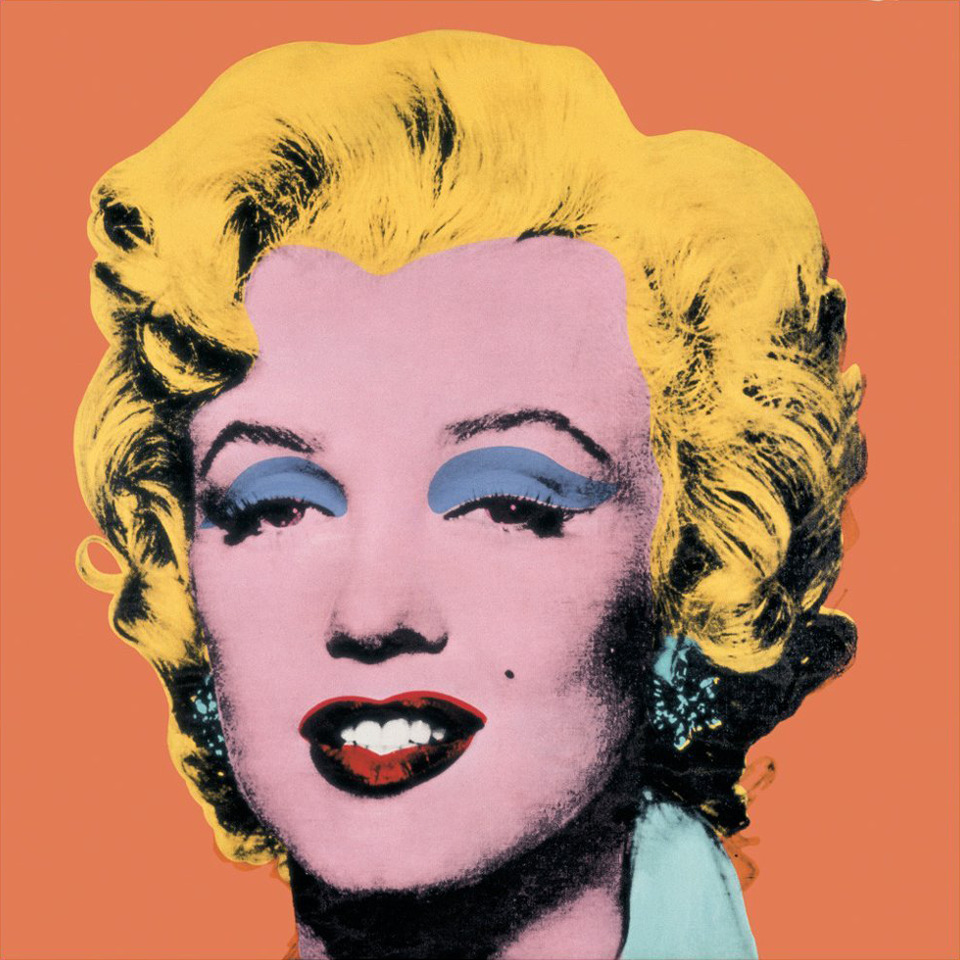
\includegraphics[width=125px]{main_files/figure-latex/1_1_orange_marilyn.jpg}
    \caption{Orange Marilyn}
    \label{fig:1_1_orange_marilyn}
  \end{subfigure}
  \hfill
  \begin{subfigure}{0.3\textwidth}
    \centering
    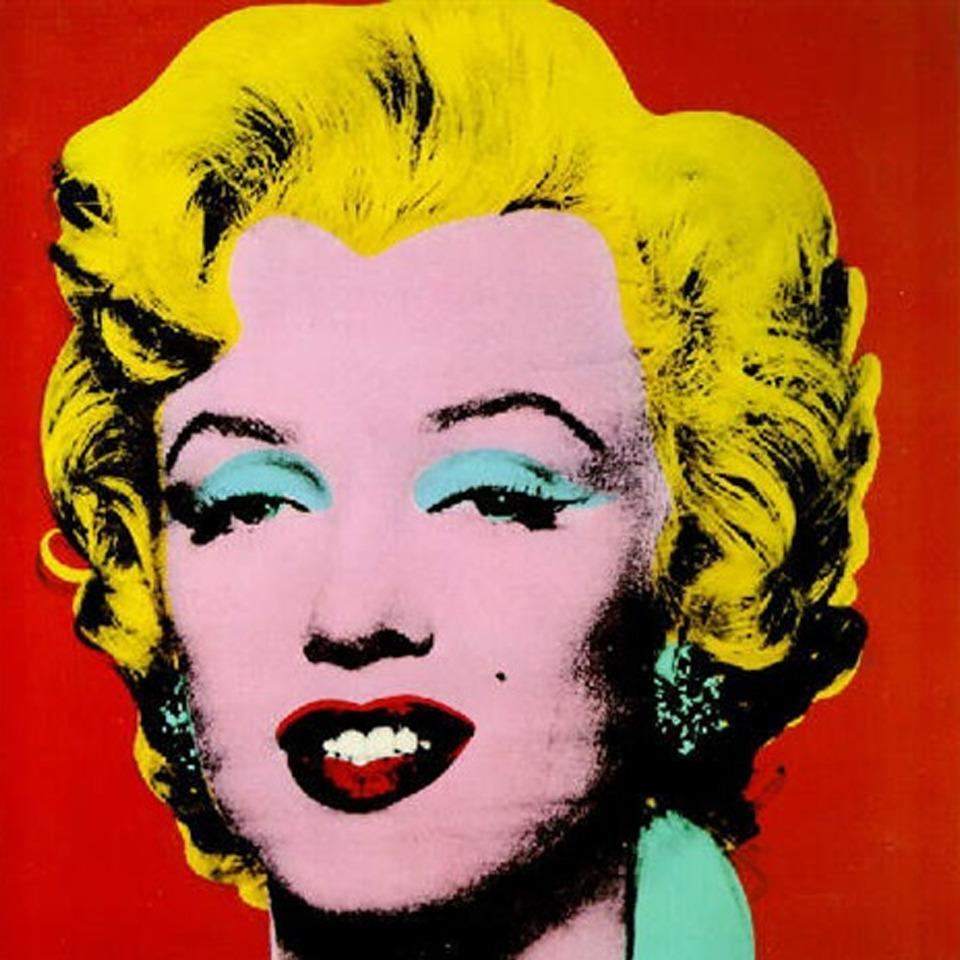
\includegraphics[width=125px]{main_files/figure-latex/1_2_red_marilyn.jpg}
    \caption{Red Marilyn}
    \label{fig:1_2_red_marilyn}
  \end{subfigure}
  \hfill
  \begin{subfigure}{0.3\textwidth}
    \centering
    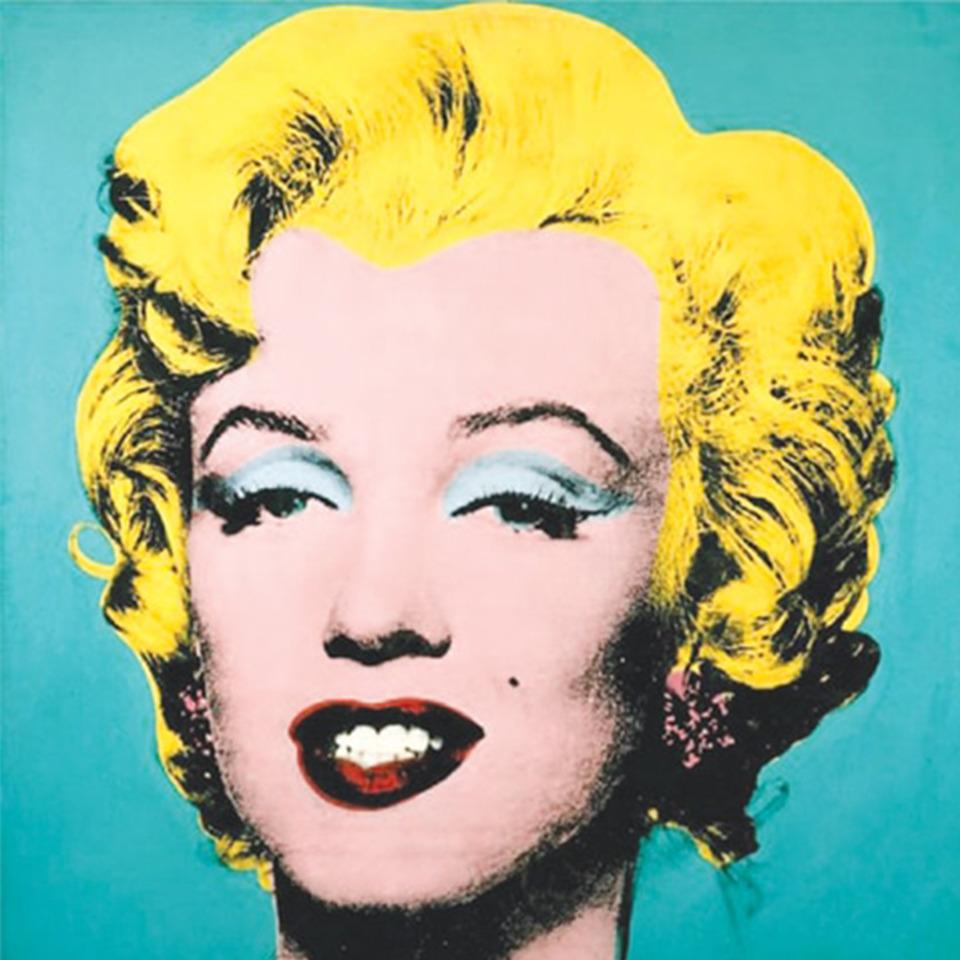
\includegraphics[width=125px]{main_files/figure-latex/1_3_turq_marilyn.jpg}
    \caption{Turquoise Marilyn}
    \label{fig:1_3_turq_marilyn}
  \end{subfigure}

  \vspace{1em}

  \begin{minipage}{0.6\textwidth}
    \centering
    \begin{subfigure}{0.45\textwidth}
      \centering
      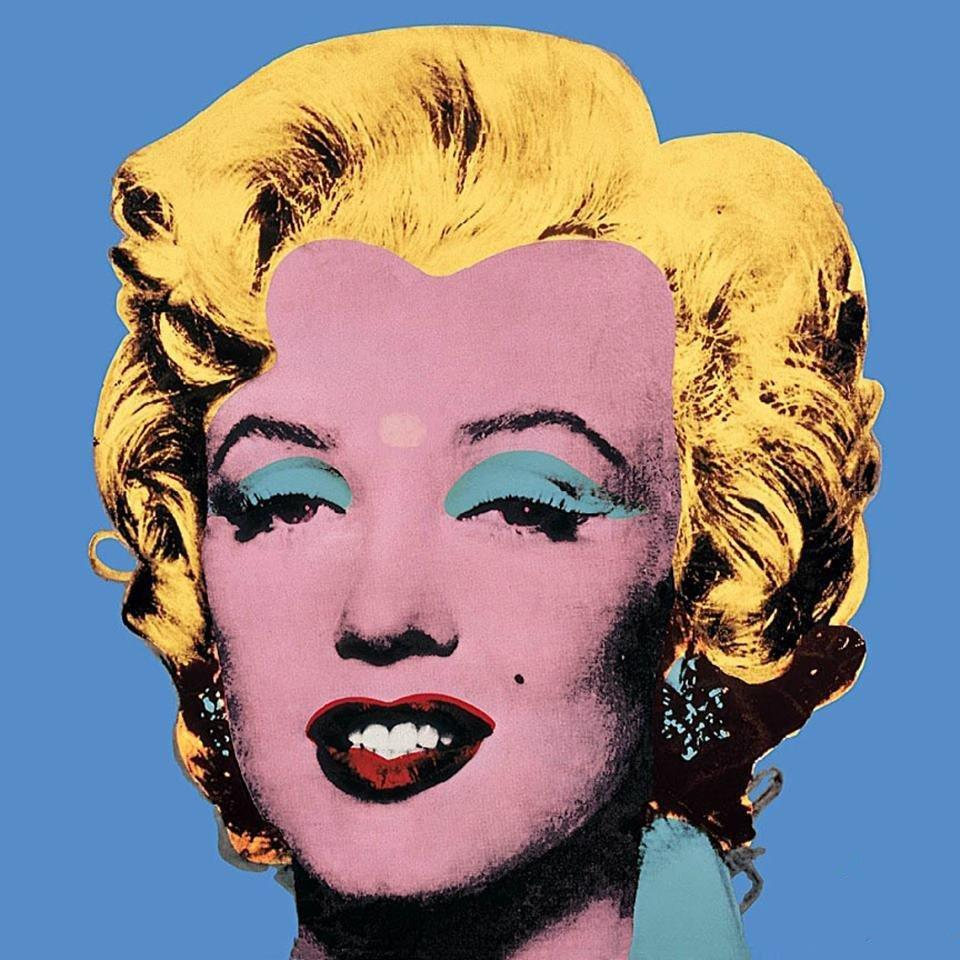
\includegraphics[width=125px]{main_files/figure-latex/1_4_blue_marilyn.jpg}
      \caption{Blue Marilyn}
      \label{fig:1_4_blue_marilyn}
    \end{subfigure}
    \hfill
    \begin{subfigure}{0.45\textwidth}
      \centering
      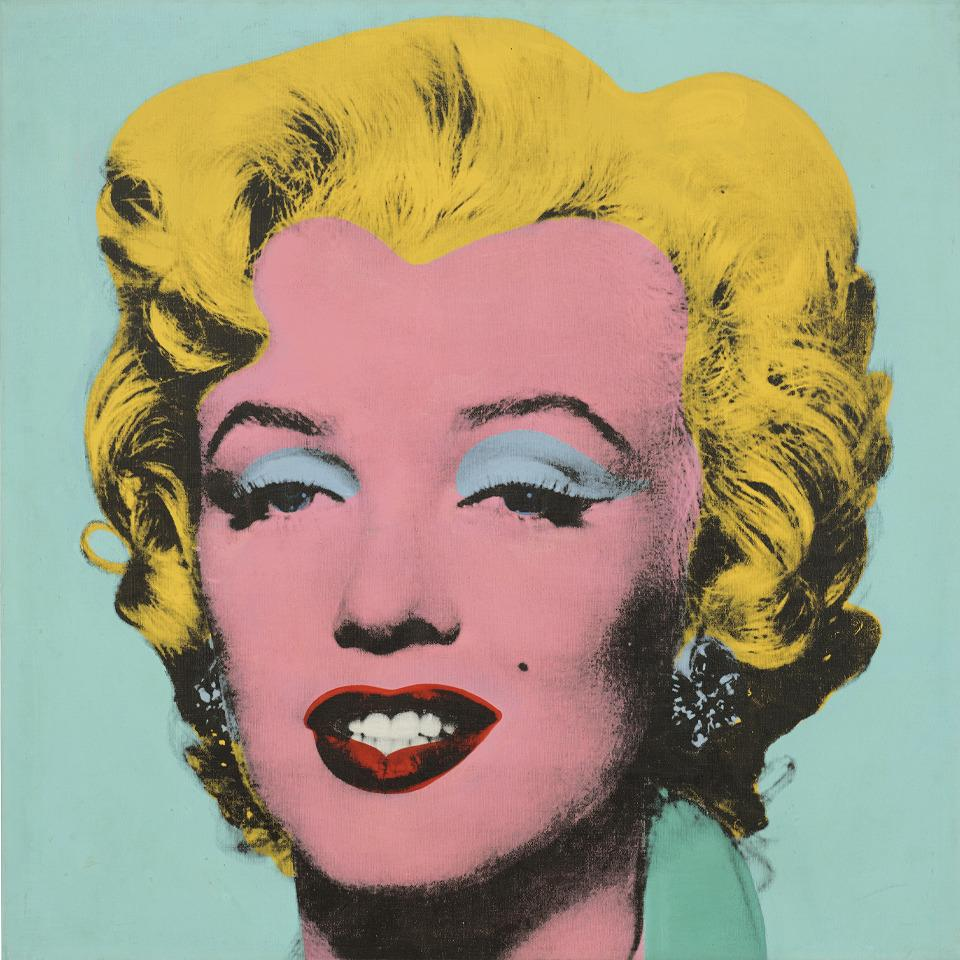
\includegraphics[width=125px]{main_files/figure-latex/1_5_eggblue_marilyn.jpg}
      \caption{Eggblue Marilyn}
      \label{fig:1_5_eggblue_marilyn}
    \end{subfigure}
  \end{minipage}

  \caption{The five portraits in Andy Warhol's "Shot Marilyns" series, each showcasing Marilyn Monroe in distinct color schemes: (a) Orange Marilyn, (b) Red Marilyn, (c) Turquoise Marilyn, (d) Blue Marilyn, and (e) Eggblue Marilyn. These variations exemplify Warhol's innovative use of color and his unique approach to portraiture. Image source: The Interior Review. Retrieved from https://www.theinteriorreview.com/story/2022/5/10/critically-assessing-warhols-shot-sage-blue-marilyn.}
  \label{fig:marilyn_variations}
\end{figure}

The name ``Shot Marilyns'' originates from an incident involving Dorothy
Podber, a performance artist and frequent visitor to The Factory. One
day, Podber, accompanied by Warhol's friend and photographer Bill Name,
observed the Marilyn portraits lined up against a wall. She asked Warhol
for permission to ``shoot'' them, which Warhol, interpreting it as a
request to photograph the artworks, granted. Unexpectedly, Podber pulled
out a revolver and fired a shot, piercing four of the five canvases
through the forehead (Ghighi 2022). This act of violence not only
created physical damage but also added a layer of historical intrigue
and controversy to Warhol's work, further embedding it into the fabric
of pop culture and art history.

In this paper, we aim to conduct a comprehensive analysis of Andy
Warhol's ``Shot Marilyns'' series using several advanced techniques.
First, we will analyze the relative conditional entropy of the pixel
color distribution in RGB (red, green, blue) space to understand the
variations in color across the different portraits. This will provide
insights into the underlying patterns and complexity of Warhol's use of
color. Next, we will create 3D scatter plots to visualize how each pixel
color is distributed in the RGB space, enabling us to observe the
distinct color palettes used in each image. We will also apply K-means
cluster analysis to identify and compare the primary color clusters
within the portraits, highlighting different regions of interest (ROI)
such as the background, hair, eyeshadow, and face. Additionally, we will
focus on digitally repairing the ``Blue Marilyn'' using K-Nearest
Neighbors to model and analyze the RGB distribution around the
gunshot-damaged area. This restoration will involve capturing the
gunshot region and using color distribution data to reconstruct the
damaged section, preserving the artwork's integrity. Through these
methods, we aim to gain a deeper understanding of Warhol's artistic
techniques and the visual impact of his ``Shot Marilyns'' series. While
our analysis strives for objectivity, we acknowledge that
interpretations of art can be inherently subjective.

\hypertarget{methods}{%
\section{Methods}\label{methods}}

An image is composed of pixels, each containing three color components:
Red (R), Green (G), and Blue (B), denoted as (R, G, B) respectively.
These components determine the intensity of their respective colors,
with each component represented by an integer value within the range of
0 to 255 in the RGB color space. Therefore, each color component is a
discrete variable capable of assuming 256 distinct values. In the
equations below, \(Y=y\) or \(X=x\) can be selected from any of the
three color components, R, G, or B. For this study, each image in the
``Shot Marilyns'' series has a resolution of 960 by 960 pixels.

\hypertarget{entropy-calculation}{%
\subsection{Entropy Calculation}\label{entropy-calculation}}

The probability of a specific color component, \(P(Y=y)\), is determined
by dividing the number of pixels with color coordinates corresponding to
that component by the total number of color components in the entire
image. The following equations illustrate the calculation of entropy,
conditional entropy, and relative conditional entropy introduced by
Shannon (1948).

The entropy of a color component \(Y\) is defined as:

\begin{equation}
  H(Y) = - \sum_{y=0}^{255} P(Y = y) \cdot \log(P(Y = y))
\end{equation}

The conditional entropy of \(Y\) given \(X\) is given by:

\begin{equation}
  H(Y|X) = \sum_{x=0}^{255} P(X = x) \cdot H(Y|X = x) = - \sum_{x=0}^{255} \sum_{y=0}^{255} P(X = x, Y = y) \log_2 \left(\frac{P(X = x, Y = y)}{P(X = x)}\right)
\end{equation}

The relative conditional entropy is calculated using the following
formula:

\begin{equation}
  HR(X|Y) = \frac{H(X|Y)}{H(X)}
\end{equation}

\hypertarget{k-means-clustering-analysis}{%
\subsection{K-Means Clustering
Analysis}\label{k-means-clustering-analysis}}

In the clustering analysis, we applied K-Means clustering to examine the
color dynamics in Andy Warhol's ``Shot Marilyns'' series. For each
image, we specified 15 clusters and used the ``k-means++''
initialization method. This initialization method, introduced by Arthur
and Vassilvitskii (2007), improves the convergence speed and accuracy of
the K-Means algorithm by spreading out the initial cluster centers. This
method is particularly effective in avoiding poor clustering results due
to the random placement of initial centroids.

Mathematically, the K-Means algorithm minimizes the following objective
function:

\begin{equation}
  J = \sum_{i=1}^{k} \sum_{x \in C_i} \| x - \mu_i \|^2
\end{equation}

where \(k\) is the number of clusters, \(C_i\) is the set of points
belonging to cluster \(i\), \(x\) represents a data point, and \(\mu_i\)
is the centroid of cluster \(i\). The ``k-means++'' algorithm
initializes the centroids by first selecting one random data point as
the first centroid. Subsequent centroids are chosen based on a
probability proportional to the squared distance from the nearest
existing centroid. This process can be expressed as:

\begin{equation}
  P(x) = \frac{D(x)^2}{\sum_{x' \in X} D(x')^2}
\end{equation}

where \(D(x)\) is the distance from the point \(x\) to the nearest
centroid already chosen.

Using this method, we applied K-Means clustering to the entire images
and specific regions of interest (ROI) in each image. The clustering
algorithm grouped pixels into clusters based on their RGB values,
effectively identifying the predominant colors in each image. This
approach allowed us to quantify and visualize the distribution of
colors, revealing the underlying color patterns and variations within
the artworks. The resulting clusters were then analyzed to understand
the prominence of specific colors across the series, as depicted in the
corresponding bar charts and ribbon visualizations. These visualizations
highlight the distinctive color schemes employed by Warhol, providing
insights into his artistic technique and color usage.

\hypertarget{roi-extraction}{%
\subsection{ROI Extraction}\label{roi-extraction}}

\hypertarget{k-nearest-neighbors-repair}{%
\subsection{K-Nearest Neighbors
Repair}\label{k-nearest-neighbors-repair}}

\hypertarget{data-description}{%
\section{Data Description}\label{data-description}}

\hypertarget{data-exploration-and-visualization-analysis}{%
\section{Data Exploration and Visualization
Analysis}\label{data-exploration-and-visualization-analysis}}

\begin{figure}[ht]
  \centering
  \begin{subfigure}{0.3\textwidth}
    \centering
    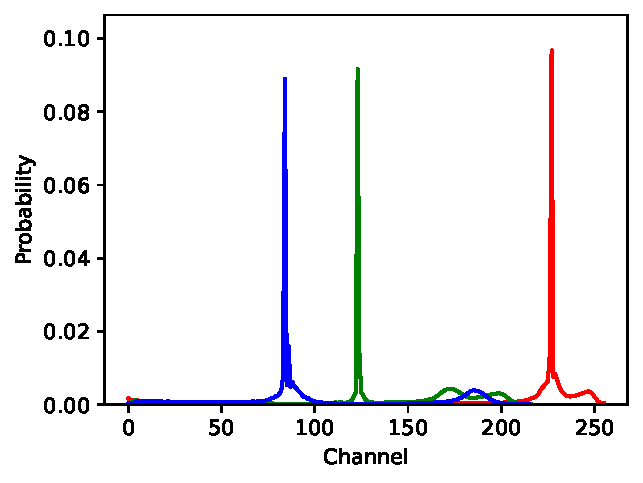
\includegraphics[width=125px]{main_files/figure-latex/2_1_orange_marilyn_dist.pdf}
    \caption{Orange Marilyn RGB Distributions}
    \label{fig:2_1_orange_marilyn_dist}
  \end{subfigure}
  \hfill
  \begin{subfigure}{0.3\textwidth}
    \centering
    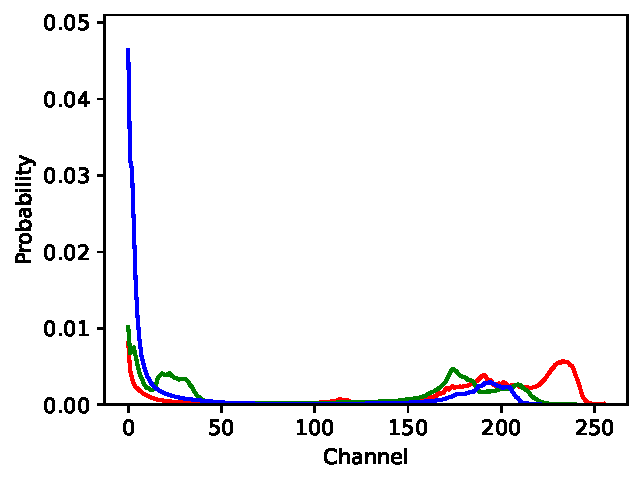
\includegraphics[width=125px]{main_files/figure-latex/2_2_red_marilyn_dist.pdf}
    \caption{Red Marilyn RGB Distributions}
    \label{fig:2_2_red_marilyn_dist}
  \end{subfigure}
  \hfill
  \begin{subfigure}{0.3\textwidth}
    \centering
    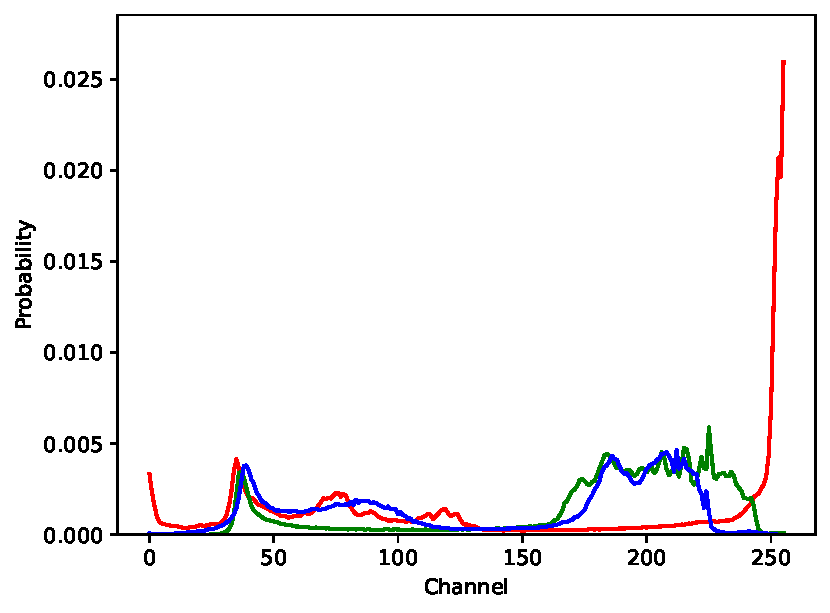
\includegraphics[width=125px]{main_files/figure-latex/2_3_turq_marilyn_dist.pdf}
    \caption{Turquoise Marilyn RGB Distributions}
    \label{fig:2_3_turq_marilyn_dist}
  \end{subfigure}

  \vspace{1em}

  \begin{minipage}{0.6\textwidth}
    \centering
    \begin{subfigure}{0.45\textwidth}
      \centering
      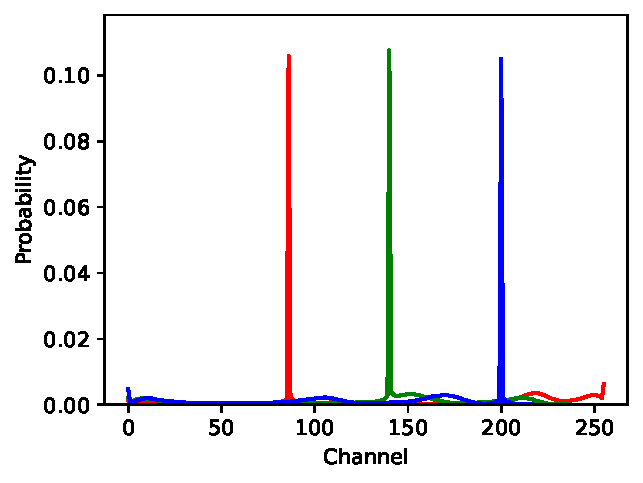
\includegraphics[width=125px]{main_files/figure-latex/2_4_blue_marilyn_dist.pdf}
      \caption{Blue Marilyn RGB Distributions}
      \label{fig:2_4_blue_marilyn_dist}
    \end{subfigure}
    \hfill
    \begin{subfigure}{0.45\textwidth}
      \centering
      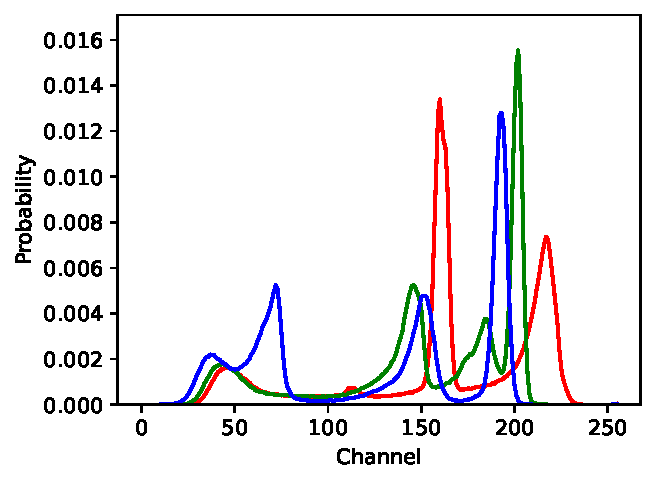
\includegraphics[width=125px]{main_files/figure-latex/2_5_eggblue_marilyn_dist.pdf}
      \caption{Eggblue Marilyn RGB Distributions}
      \label{fig:2_5_eggblue_marilyn_dist}
    \end{subfigure}
  \end{minipage}

  \caption{Distributions of values of Red, Green, and Blue channels for five images with all pixels}
  \label{fig:marilyn_dist}
\end{figure}

\begin{figure}[ht]
  \centering
  \begin{subfigure}{0.3\textwidth}
    \centering
    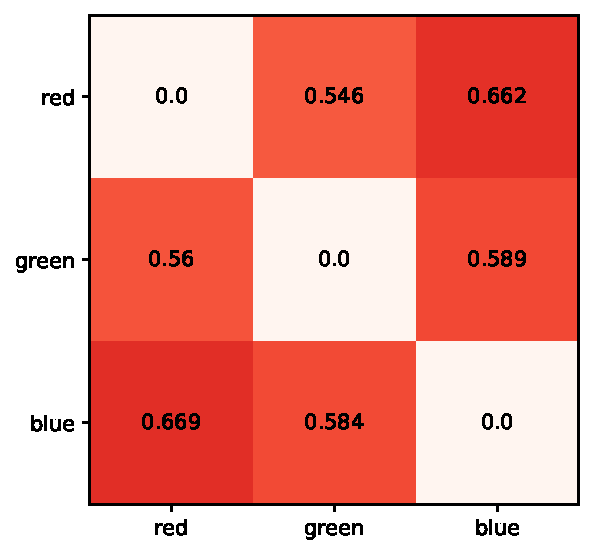
\includegraphics[width=125px]{main_files/figure-latex/3_1_orange_marilyn_entropy.pdf}
    \caption{Orange Marilyn Relative Conditional Entropy}
    \label{fig:3_1_orange_marilyn_entropy}
  \end{subfigure}
  \hfill
  \begin{subfigure}{0.3\textwidth}
    \centering
    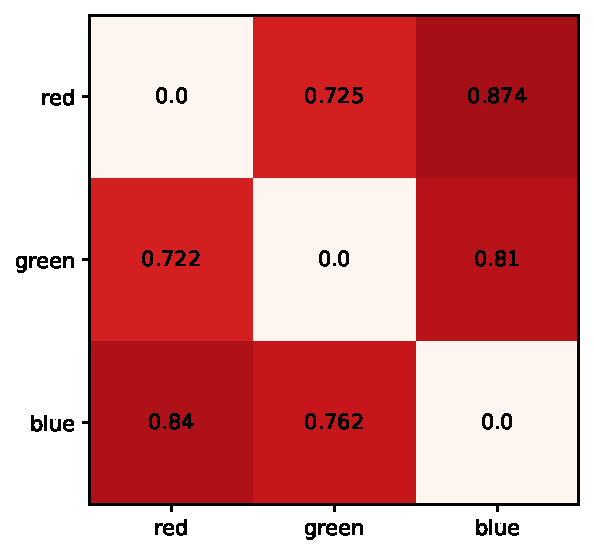
\includegraphics[width=125px]{main_files/figure-latex/3_2_red_marilyn_entropy.pdf}
    \caption{Red Marilyn Relative Conditional Entropy}
    \label{fig:3_2_red_marilyn_entropy}
  \end{subfigure}
  \hfill
  \begin{subfigure}{0.3\textwidth}
    \centering
    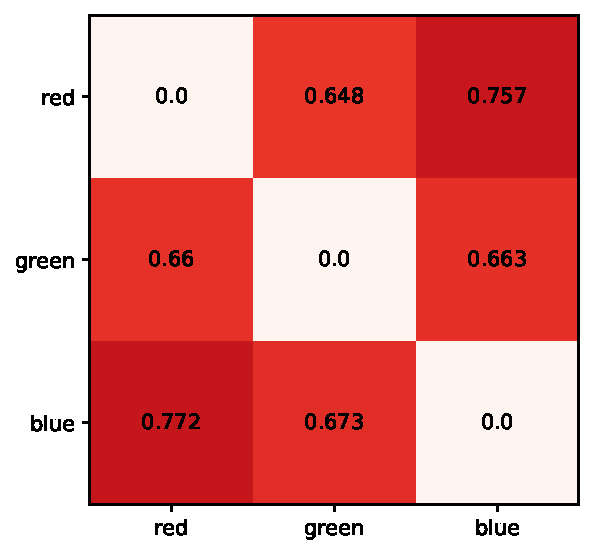
\includegraphics[width=125px]{main_files/figure-latex/3_3_turq_marilyn_entropy.pdf}
    \caption{Turquoise Marilyn Relative Conditional Entropy}
    \label{fig:3_3_turq_marilyn_entropy}
  \end{subfigure}

  \vspace{1em} % Add some vertical space between rows

  \begin{minipage}{0.6\textwidth}
    \centering
    \begin{subfigure}{0.45\textwidth}
      \centering
      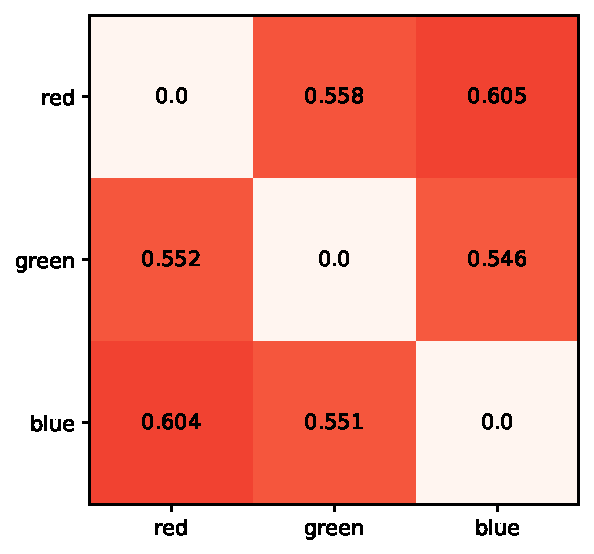
\includegraphics[width=125px]{main_files/figure-latex/3_4_blue_marilyn_entropy.pdf}
      \caption{Blue Marilyn Relative Conditional Entropy}
      \label{fig:3_4_blue_marilyn_entropy}
    \end{subfigure}
    \hfill
    \begin{subfigure}{0.45\textwidth}
      \centering
      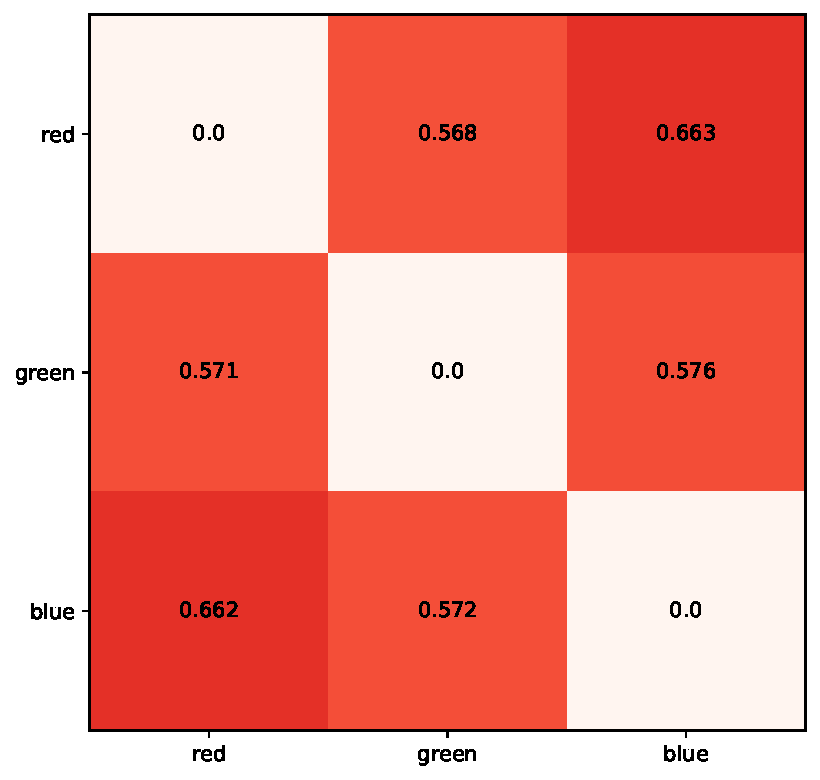
\includegraphics[width=125px]{main_files/figure-latex/3_5_eggblue_marilyn_entropy.pdf}
      \caption{Eggblue Marilyn Relative Conditional Entropy}
      \label{fig:3_5_eggblue_marilyn_entropy}
    \end{subfigure}
  \end{minipage}

  \caption{The relative conditional entropy values among the red, green, and blue coordinates of pixels}
  \label{fig:marilyn_entropy}
\end{figure}

\hypertarget{clustering-based-on-whole-images}{%
\section{Clustering based on Whole
Images}\label{clustering-based-on-whole-images}}

The figures below display the RGB space occupied by the pixels of
various Marilyn paintings from four different angles. Each subplot
reveals the distribution and density of pixel colors in the 3D RGB color
space, providing insights into the color composition and variations
within the images.

\begin{figure}[ht]
  \centering
  \begin{subfigure}{0.45\textwidth}
    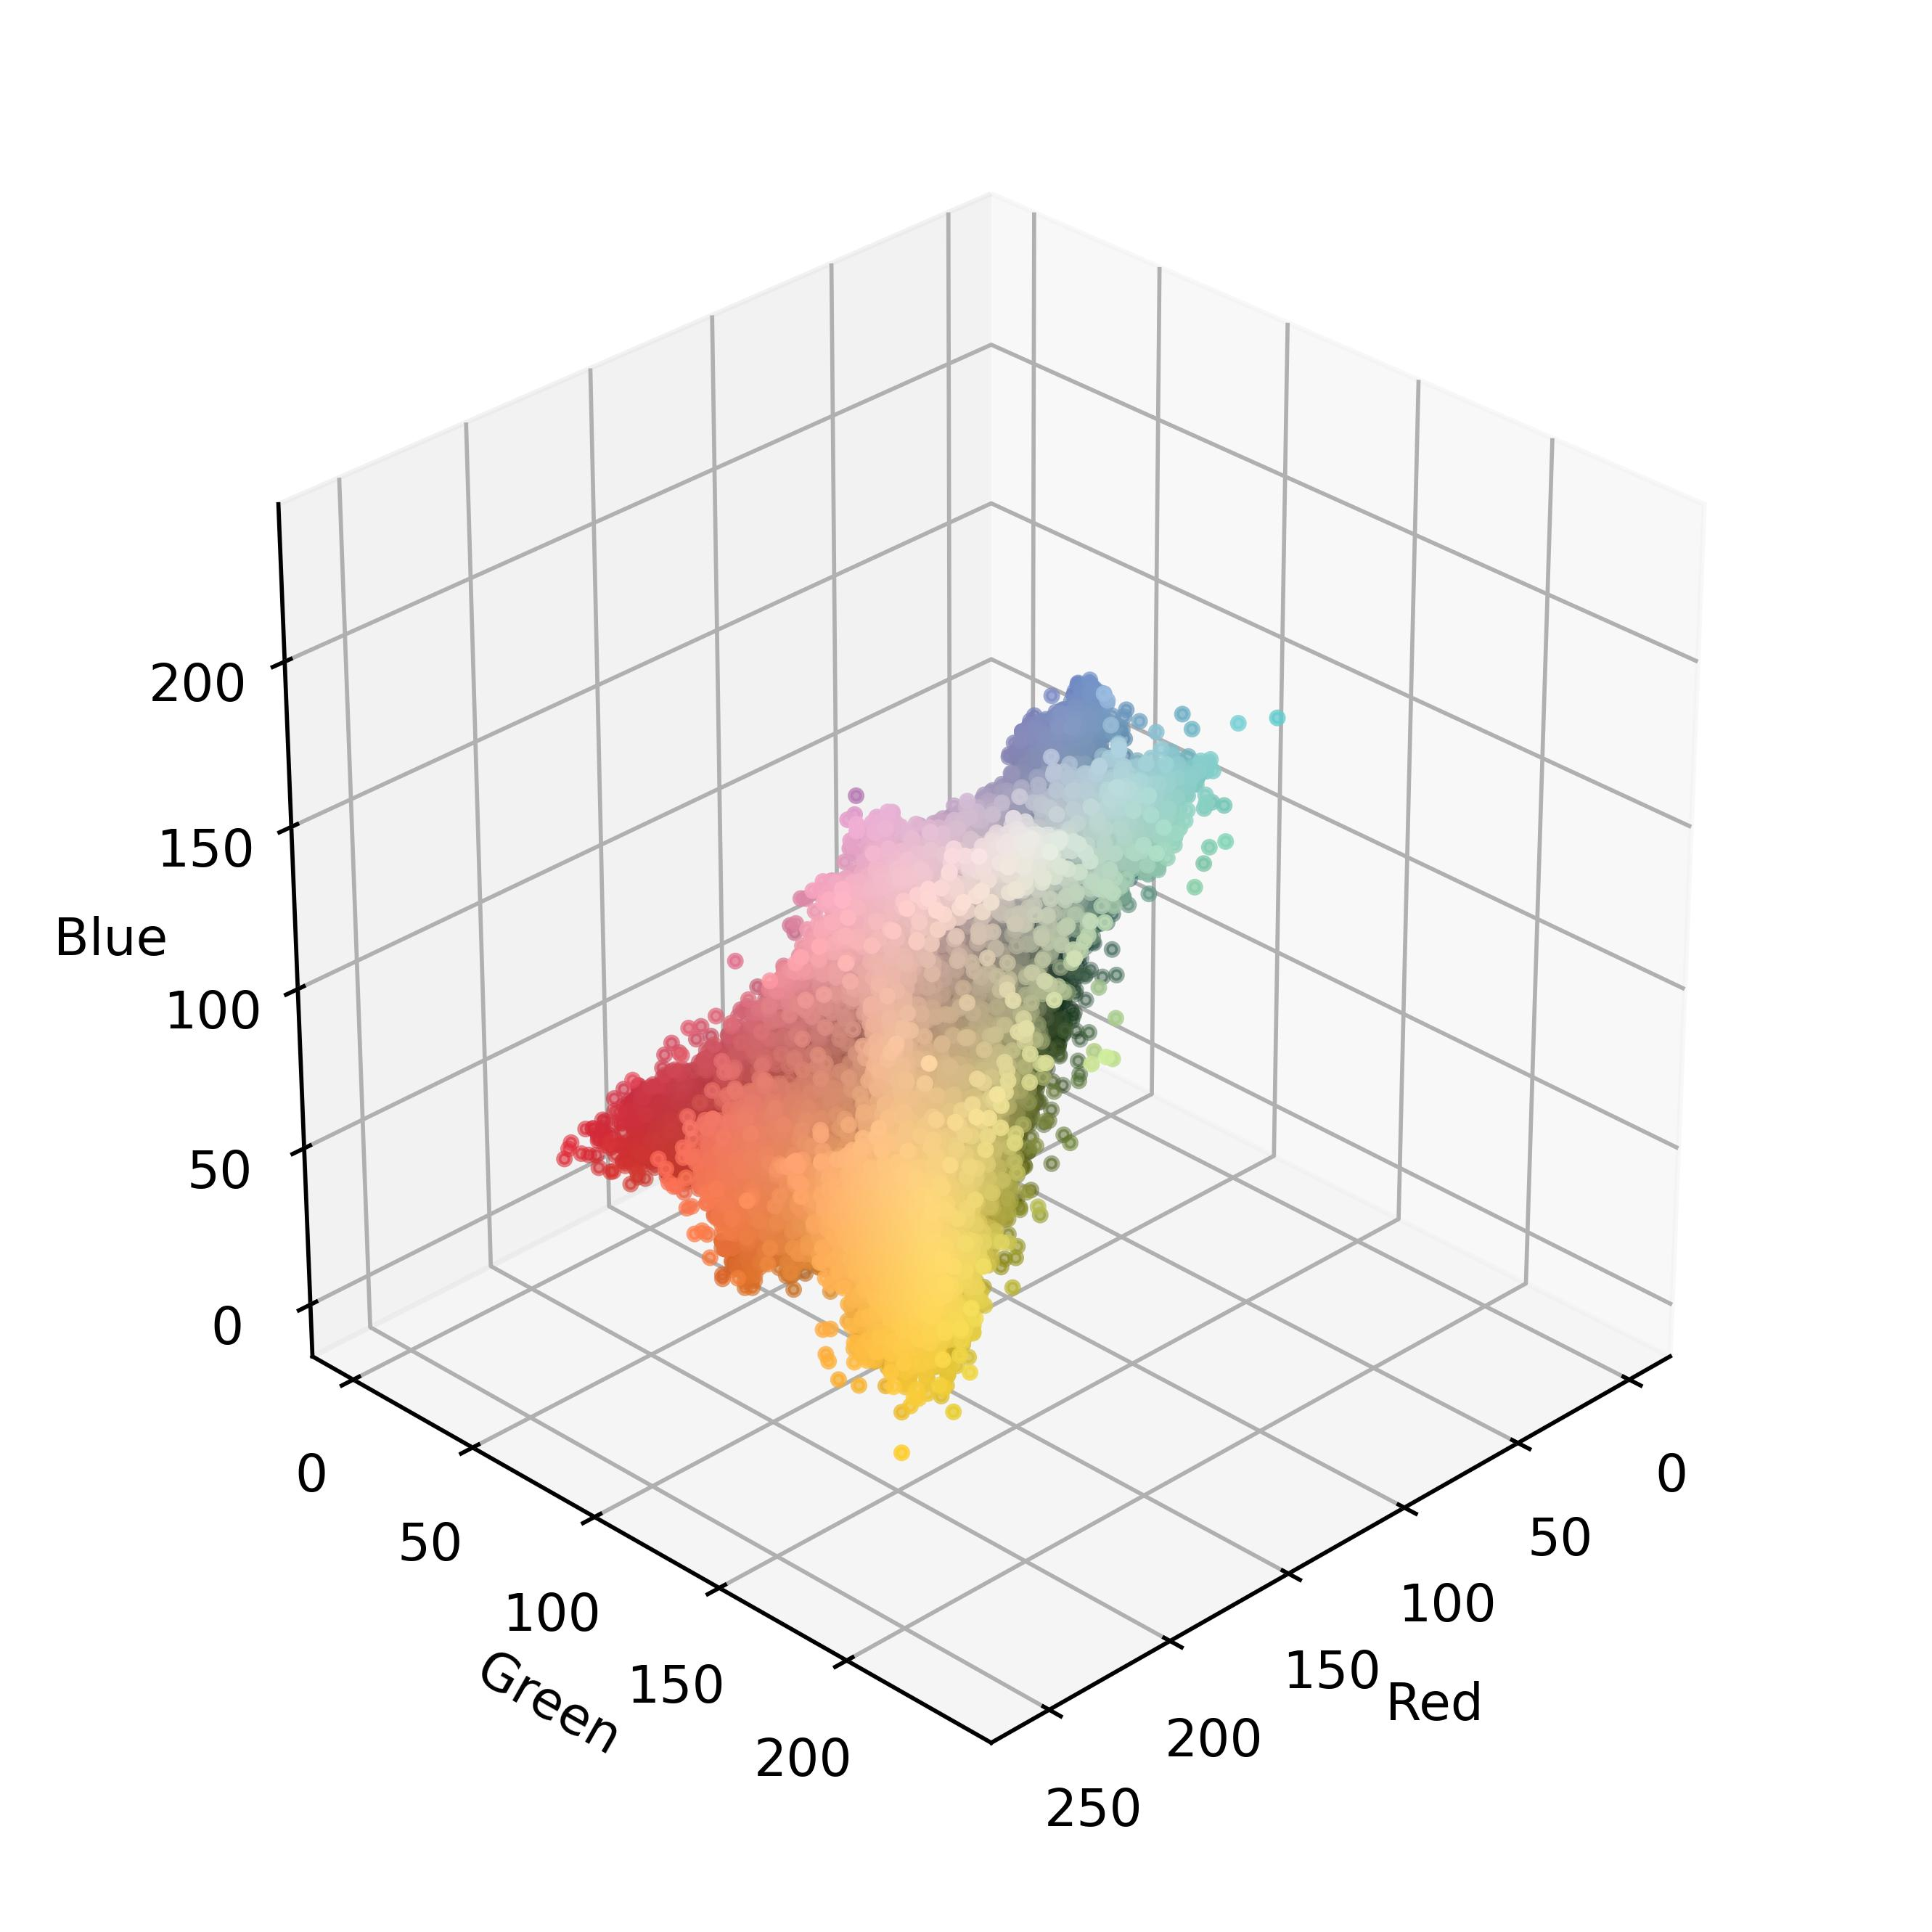
\includegraphics[width=\textwidth]{main_files/figure-latex/4_1_orange_marilyn_original_scatter.jpg}
    \caption{Orange Marilyn RGB Space - 30 \degree elevation, 45 \degree azimuth}
    \label{fig:4_1_orange_marilyn_original_scatter}
  \end{subfigure}
  \hfill
  \begin{subfigure}{0.45\textwidth}
    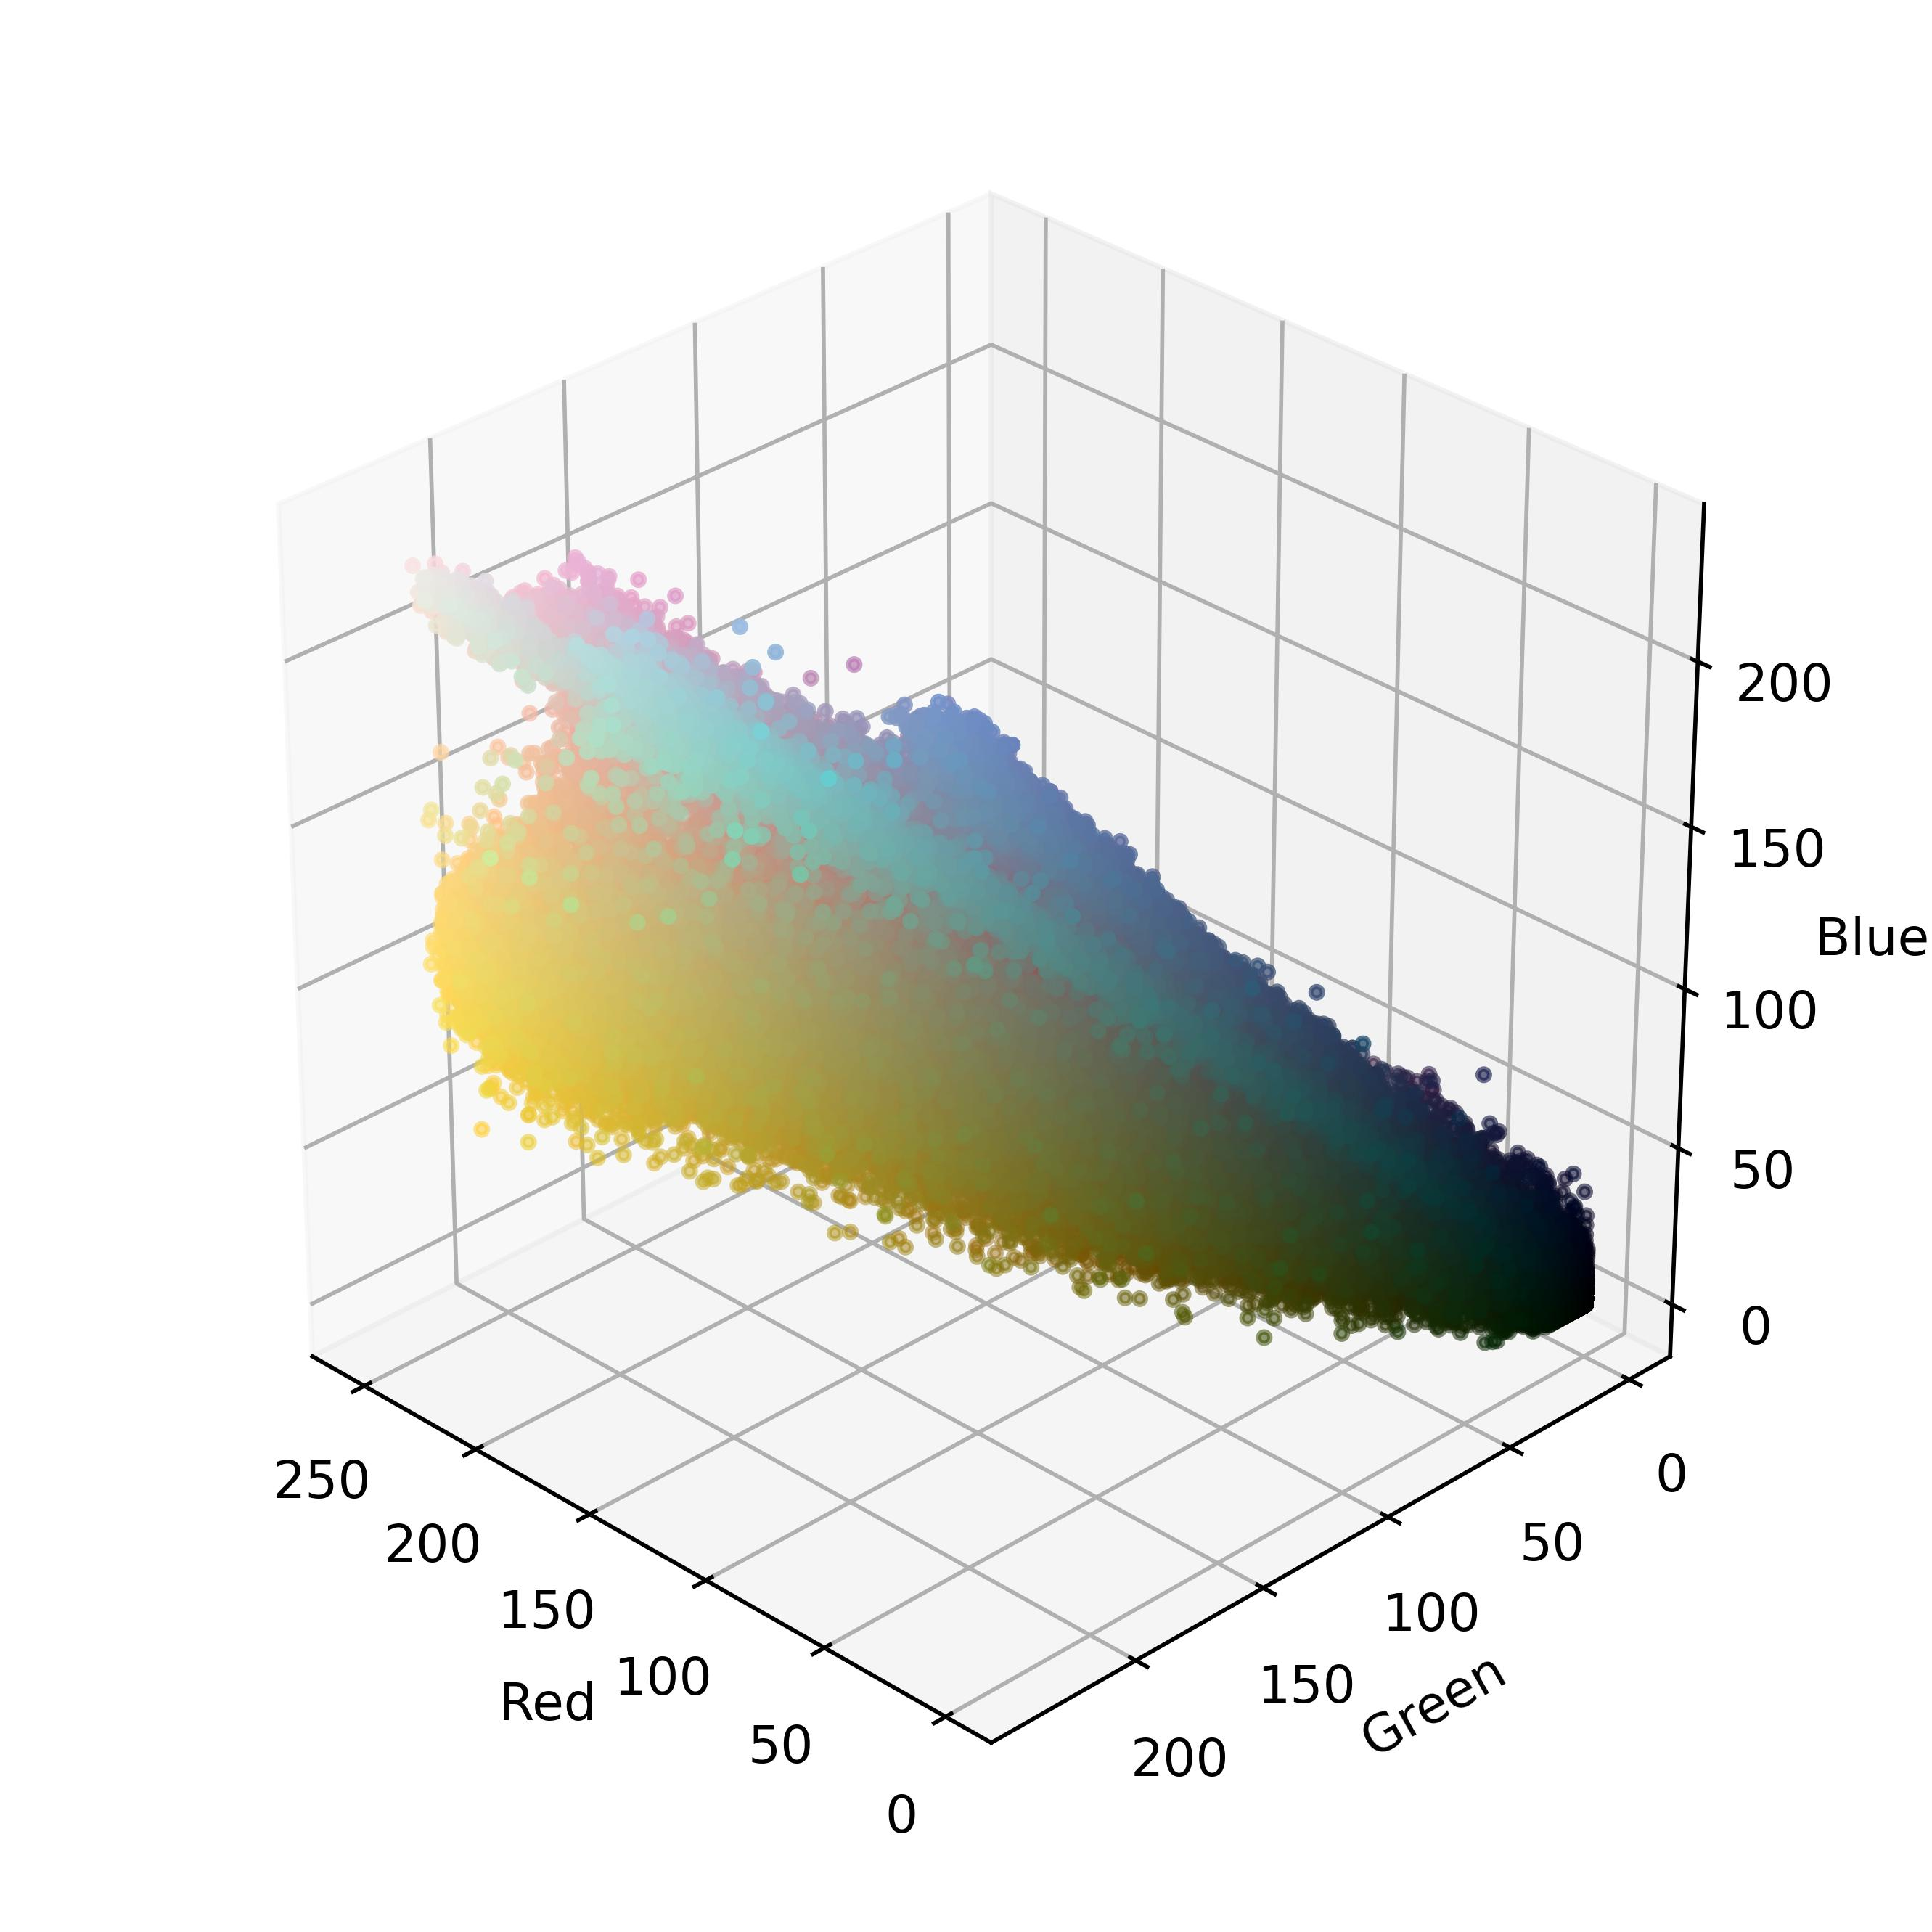
\includegraphics[width=\textwidth]{main_files/figure-latex/4_2_orange_marilyn_original_scatter.jpg}
    \caption{Orange Marilyn RGB Space - 30 \degree elevation, 135 \degree azimuth}
    \label{fig:4_2_orange_marilyn_original_scatter}
  \end{subfigure}
  \label{fig:orange_marilyn_original_scatter_1}
\end{figure}

\begin{figure}[ht]\ContinuedFloat
  \centering
  \begin{subfigure}{0.45\textwidth}
    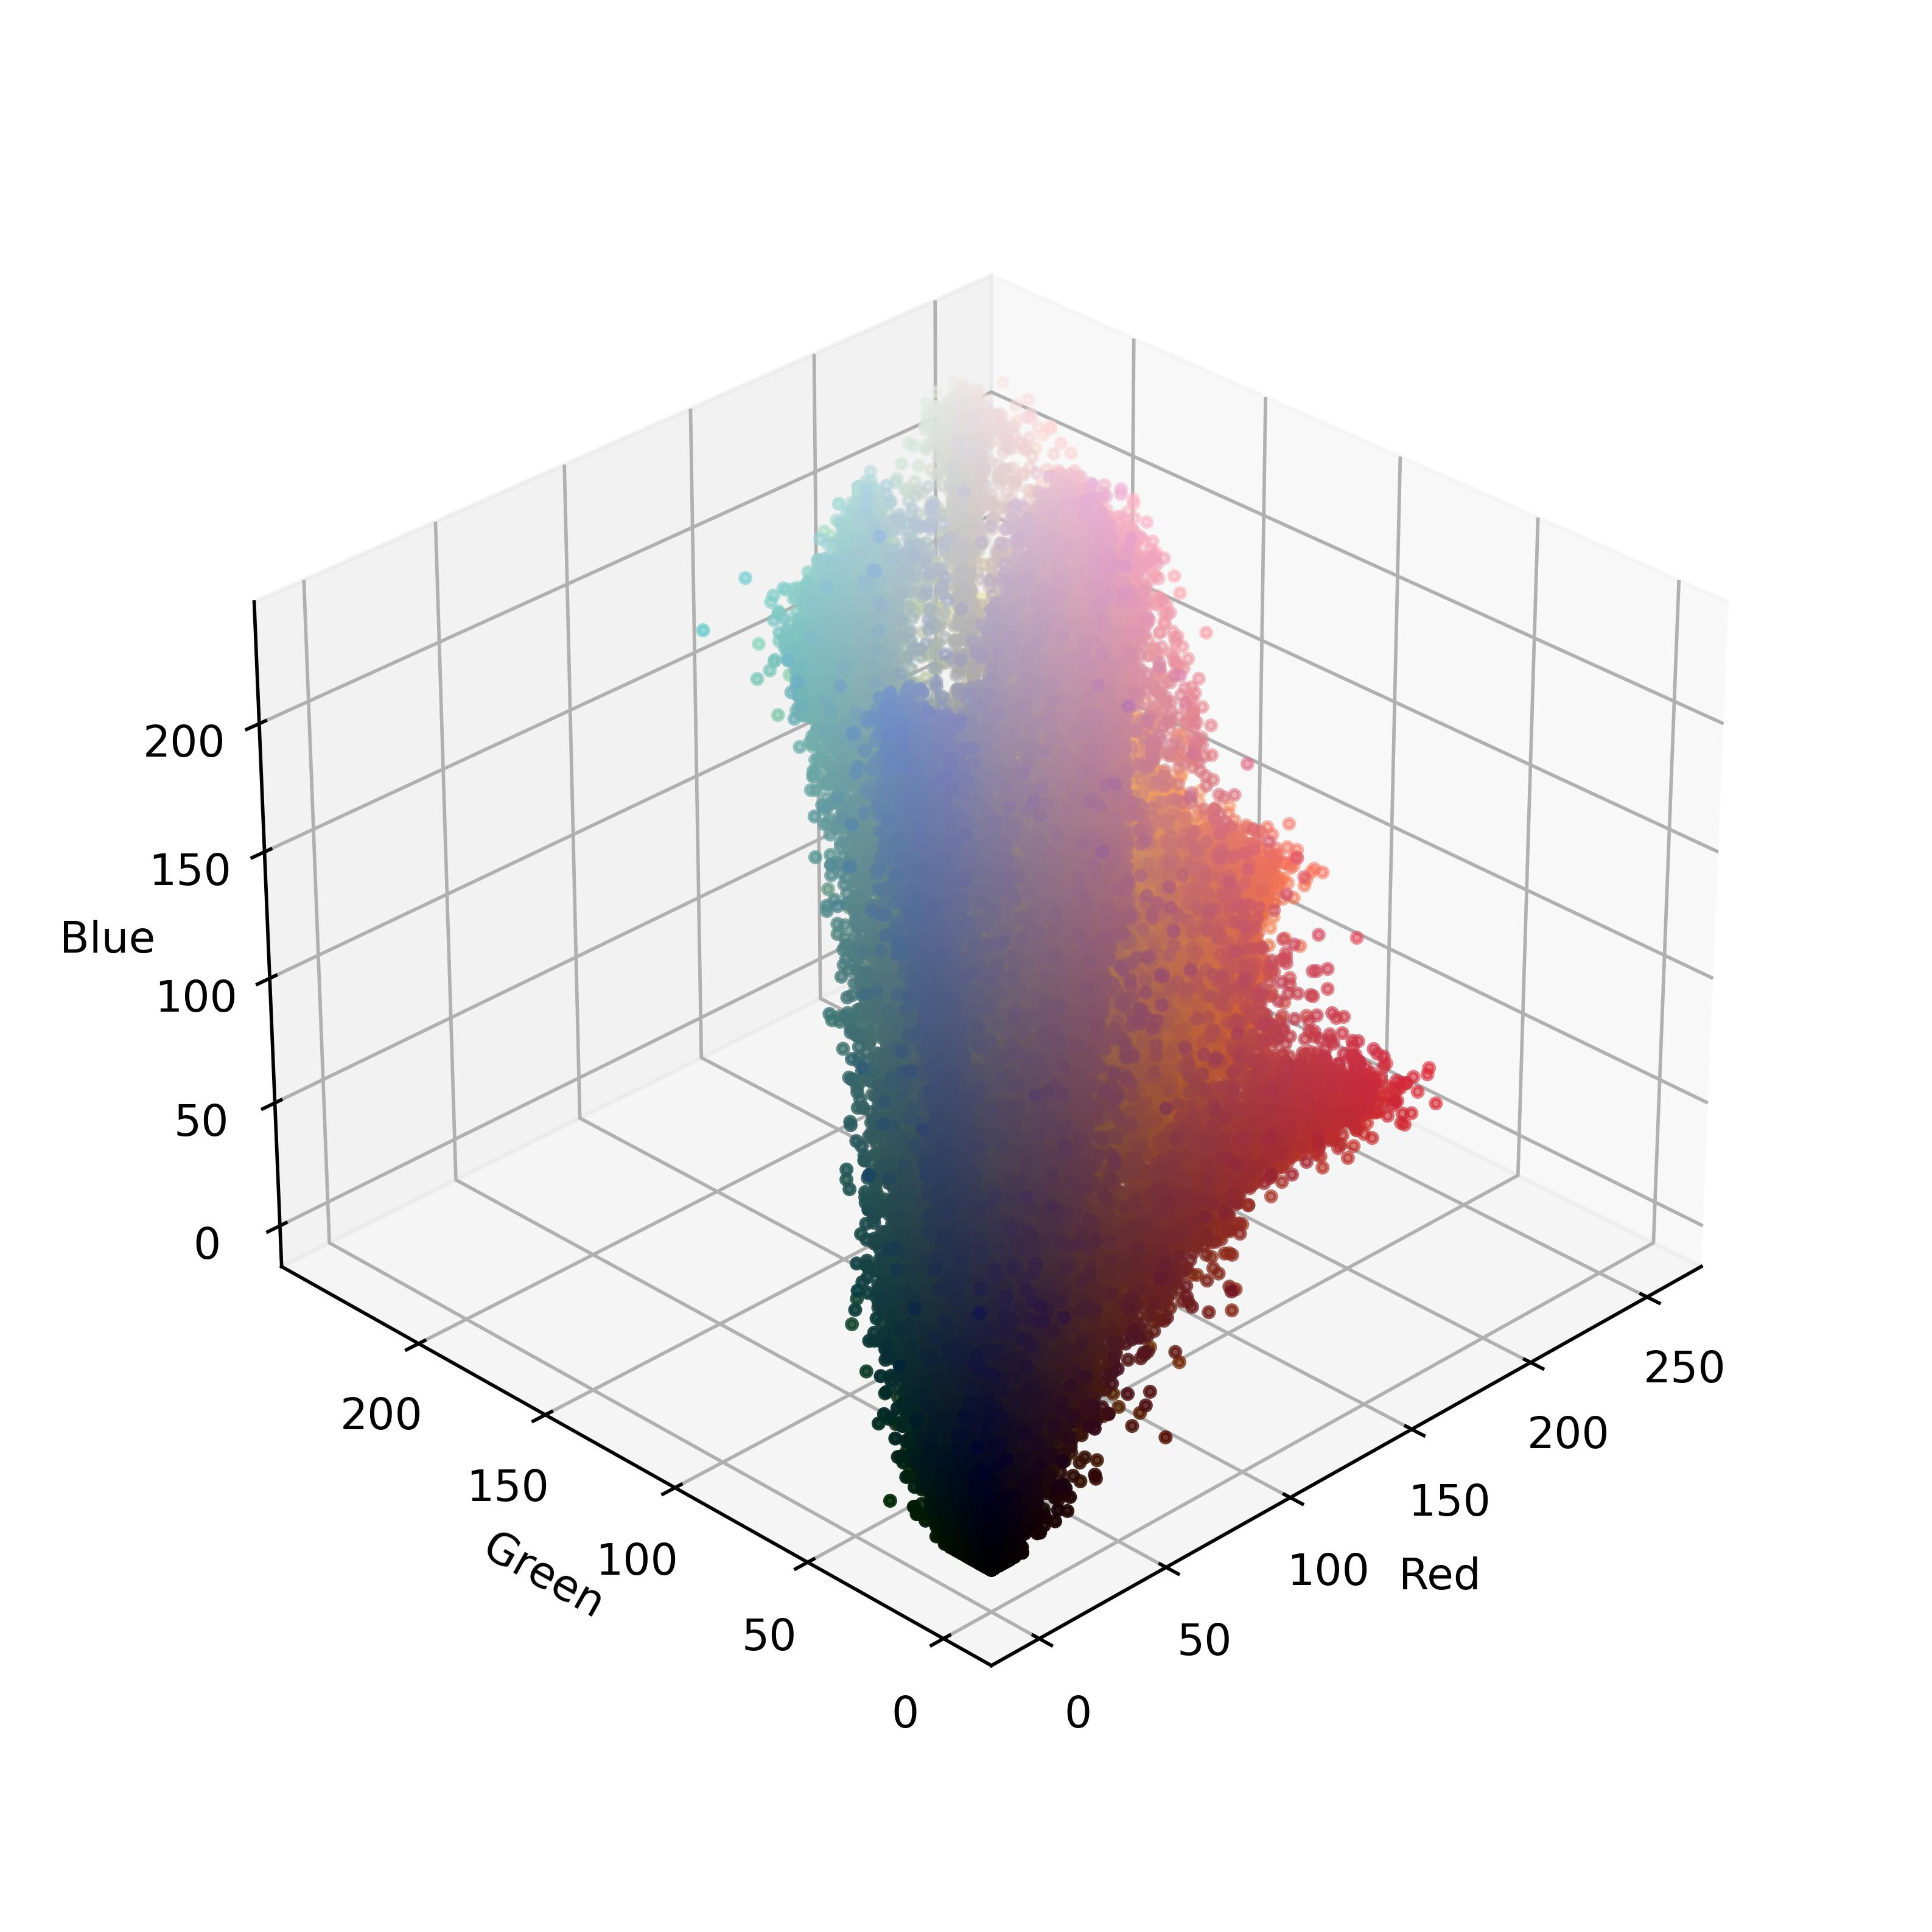
\includegraphics[width=\textwidth]{main_files/figure-latex/4_3_orange_marilyn_original_scatter.jpg}
    \caption{Orange Marilyn RGB Space - 30 \degree elevation, 225 \degree azimuth}
    \label{fig:4_3_orange_marilyn_original_scatter}
  \end{subfigure}
  \hfill
  \begin{subfigure}{0.45\textwidth}
    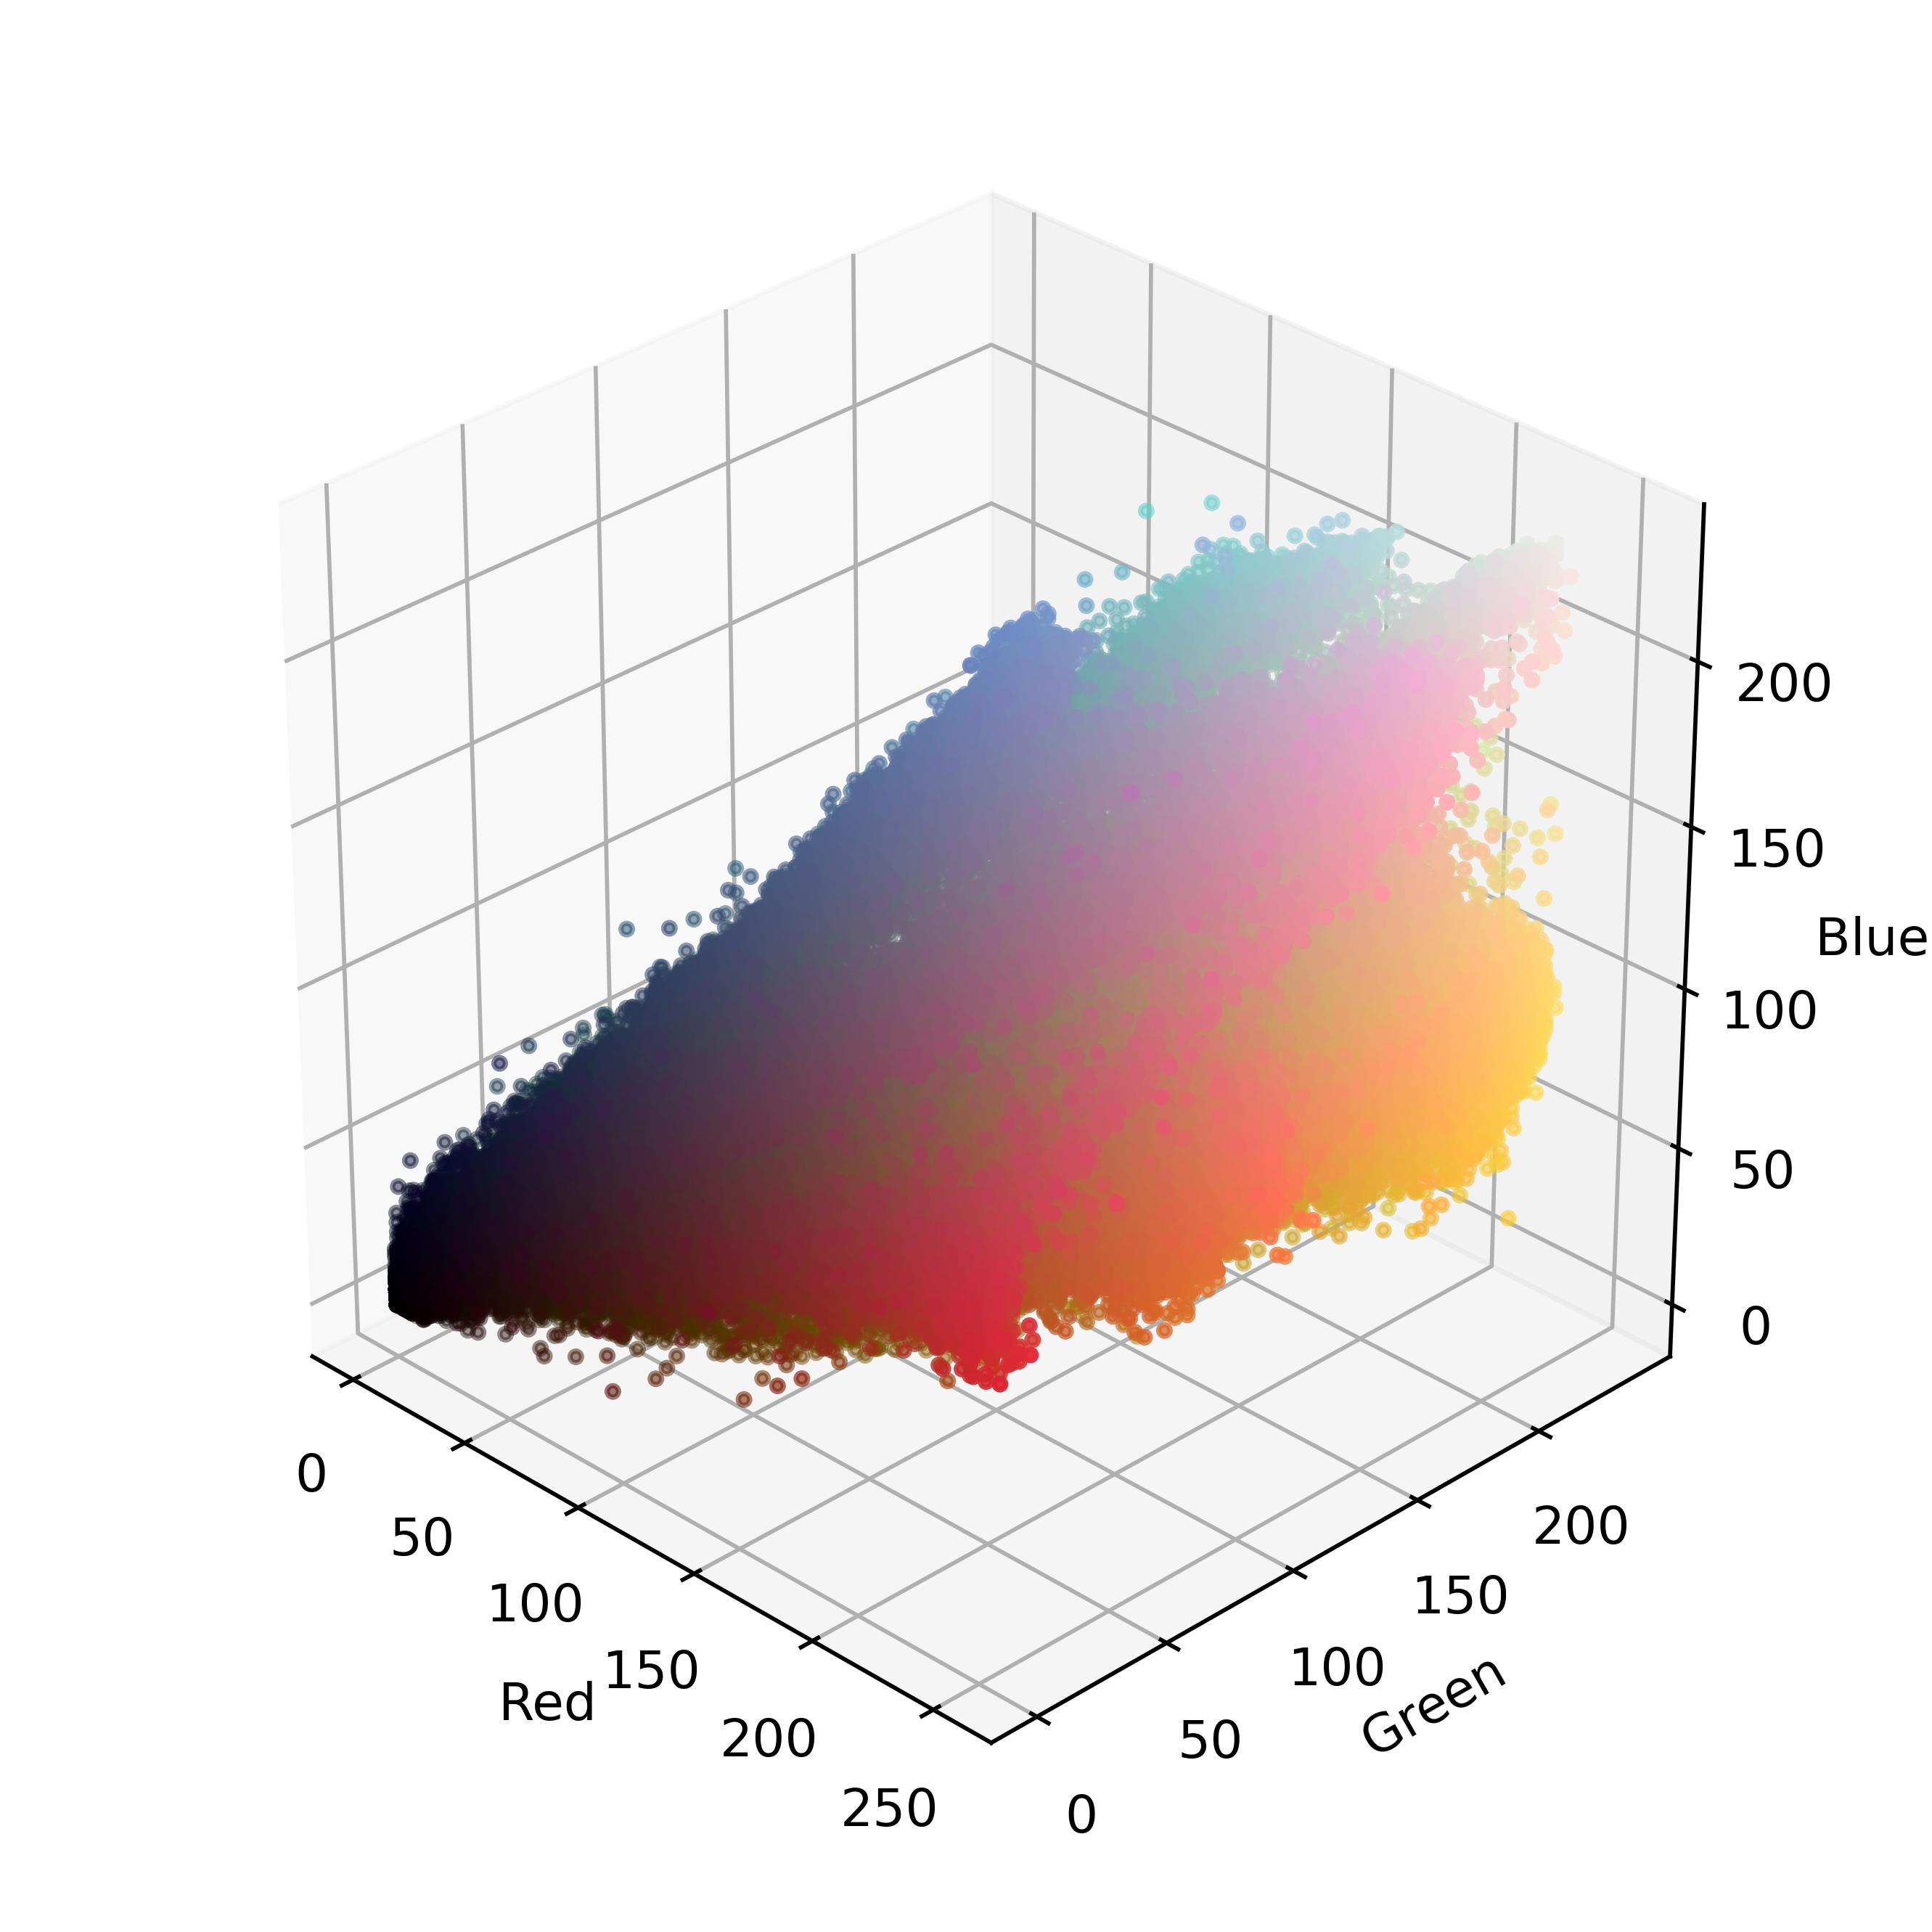
\includegraphics[width=\textwidth]{main_files/figure-latex/4_4_orange_marilyn_original_scatter.jpg}
    \caption{Orange Marilyn RGB Space - 30 \degree elevation, 315 \degree azimuth}
    \label{fig:4_4_orange_marilyn_original_scatter}
  \end{subfigure}
  \caption{The RGB space occupied by the pixels for the entire image of Orange Marilyn, showing different angles: (a) 30 \degree elevation, 45 \degree azimuth, (b) 30 \degree elevation, 135 \degree azimuth, (c) 30 \degree elevation, 225 \degree azimuth, (d) 30 \degree elevation, 315 \degree azimuth. These variations highlight the color distribution within the artwork.}
  \label{fig:orange_marilyn_original_scatter_2}
\end{figure}

Figure 4 displays the RGB space of ``Orange Marilyn'' from four
different angles. In (a), the density of pixels representing the
background part of the image is shown, revealing a balanced mix of
colors including orange, yellow, pink, red, and blue. These colors
reflect the different dominant areas of the painting: the orange
background, yellow hair, pink face, red lips, and blue eye shades. The
shape of the 3D scatter plot in (a) indicates a broad, dispersed
distribution of colors, showing the diverse color use in the background
and facial features.

In (b), the plot illustrates how colors are distributed from darker
pixels at the bottom to brighter pixels at the top, highlighting shading
gradients. This gradient reflects the shading around Marilyn's facial
features and hair, adding depth to the portrait. The darker pixels
likely represent shadows in the hair and facial contours, while the
brighter pixels correspond to highlights on her face and hair.

In (c), the concentration of the brightest pixels is evident, showing
specific groupings likely related to prominent features. This highlights
the intense colors used in Marilyn's lips, eyes, and other facial
highlights. The plot suggests a focused clustering of bright colors,
indicating areas where Warhol applied more vivid hues to draw attention.

In (d), the color distribution from dark to light is presented from a
different angle, allowing us to observe the distribution of colors in
areas such as hair and eye shades with less red. This provides a
different perspective on the artwork's color dynamics, showing how the
turquoise and yellow shades in the hair and the blue in the eyes are
distributed. The shapes in (b) through (d) all reflect a similar
elongated form, resembling a long funnel, showing a clear gradient from
dark to light colors. This consistent shape across different angles
highlights the structured way Warhol applied color to create depth and
contrast in the ``Orange Marilyn'' painting.

\begin{figure}[ht]
  \centering
  \begin{subfigure}{0.45\textwidth}
    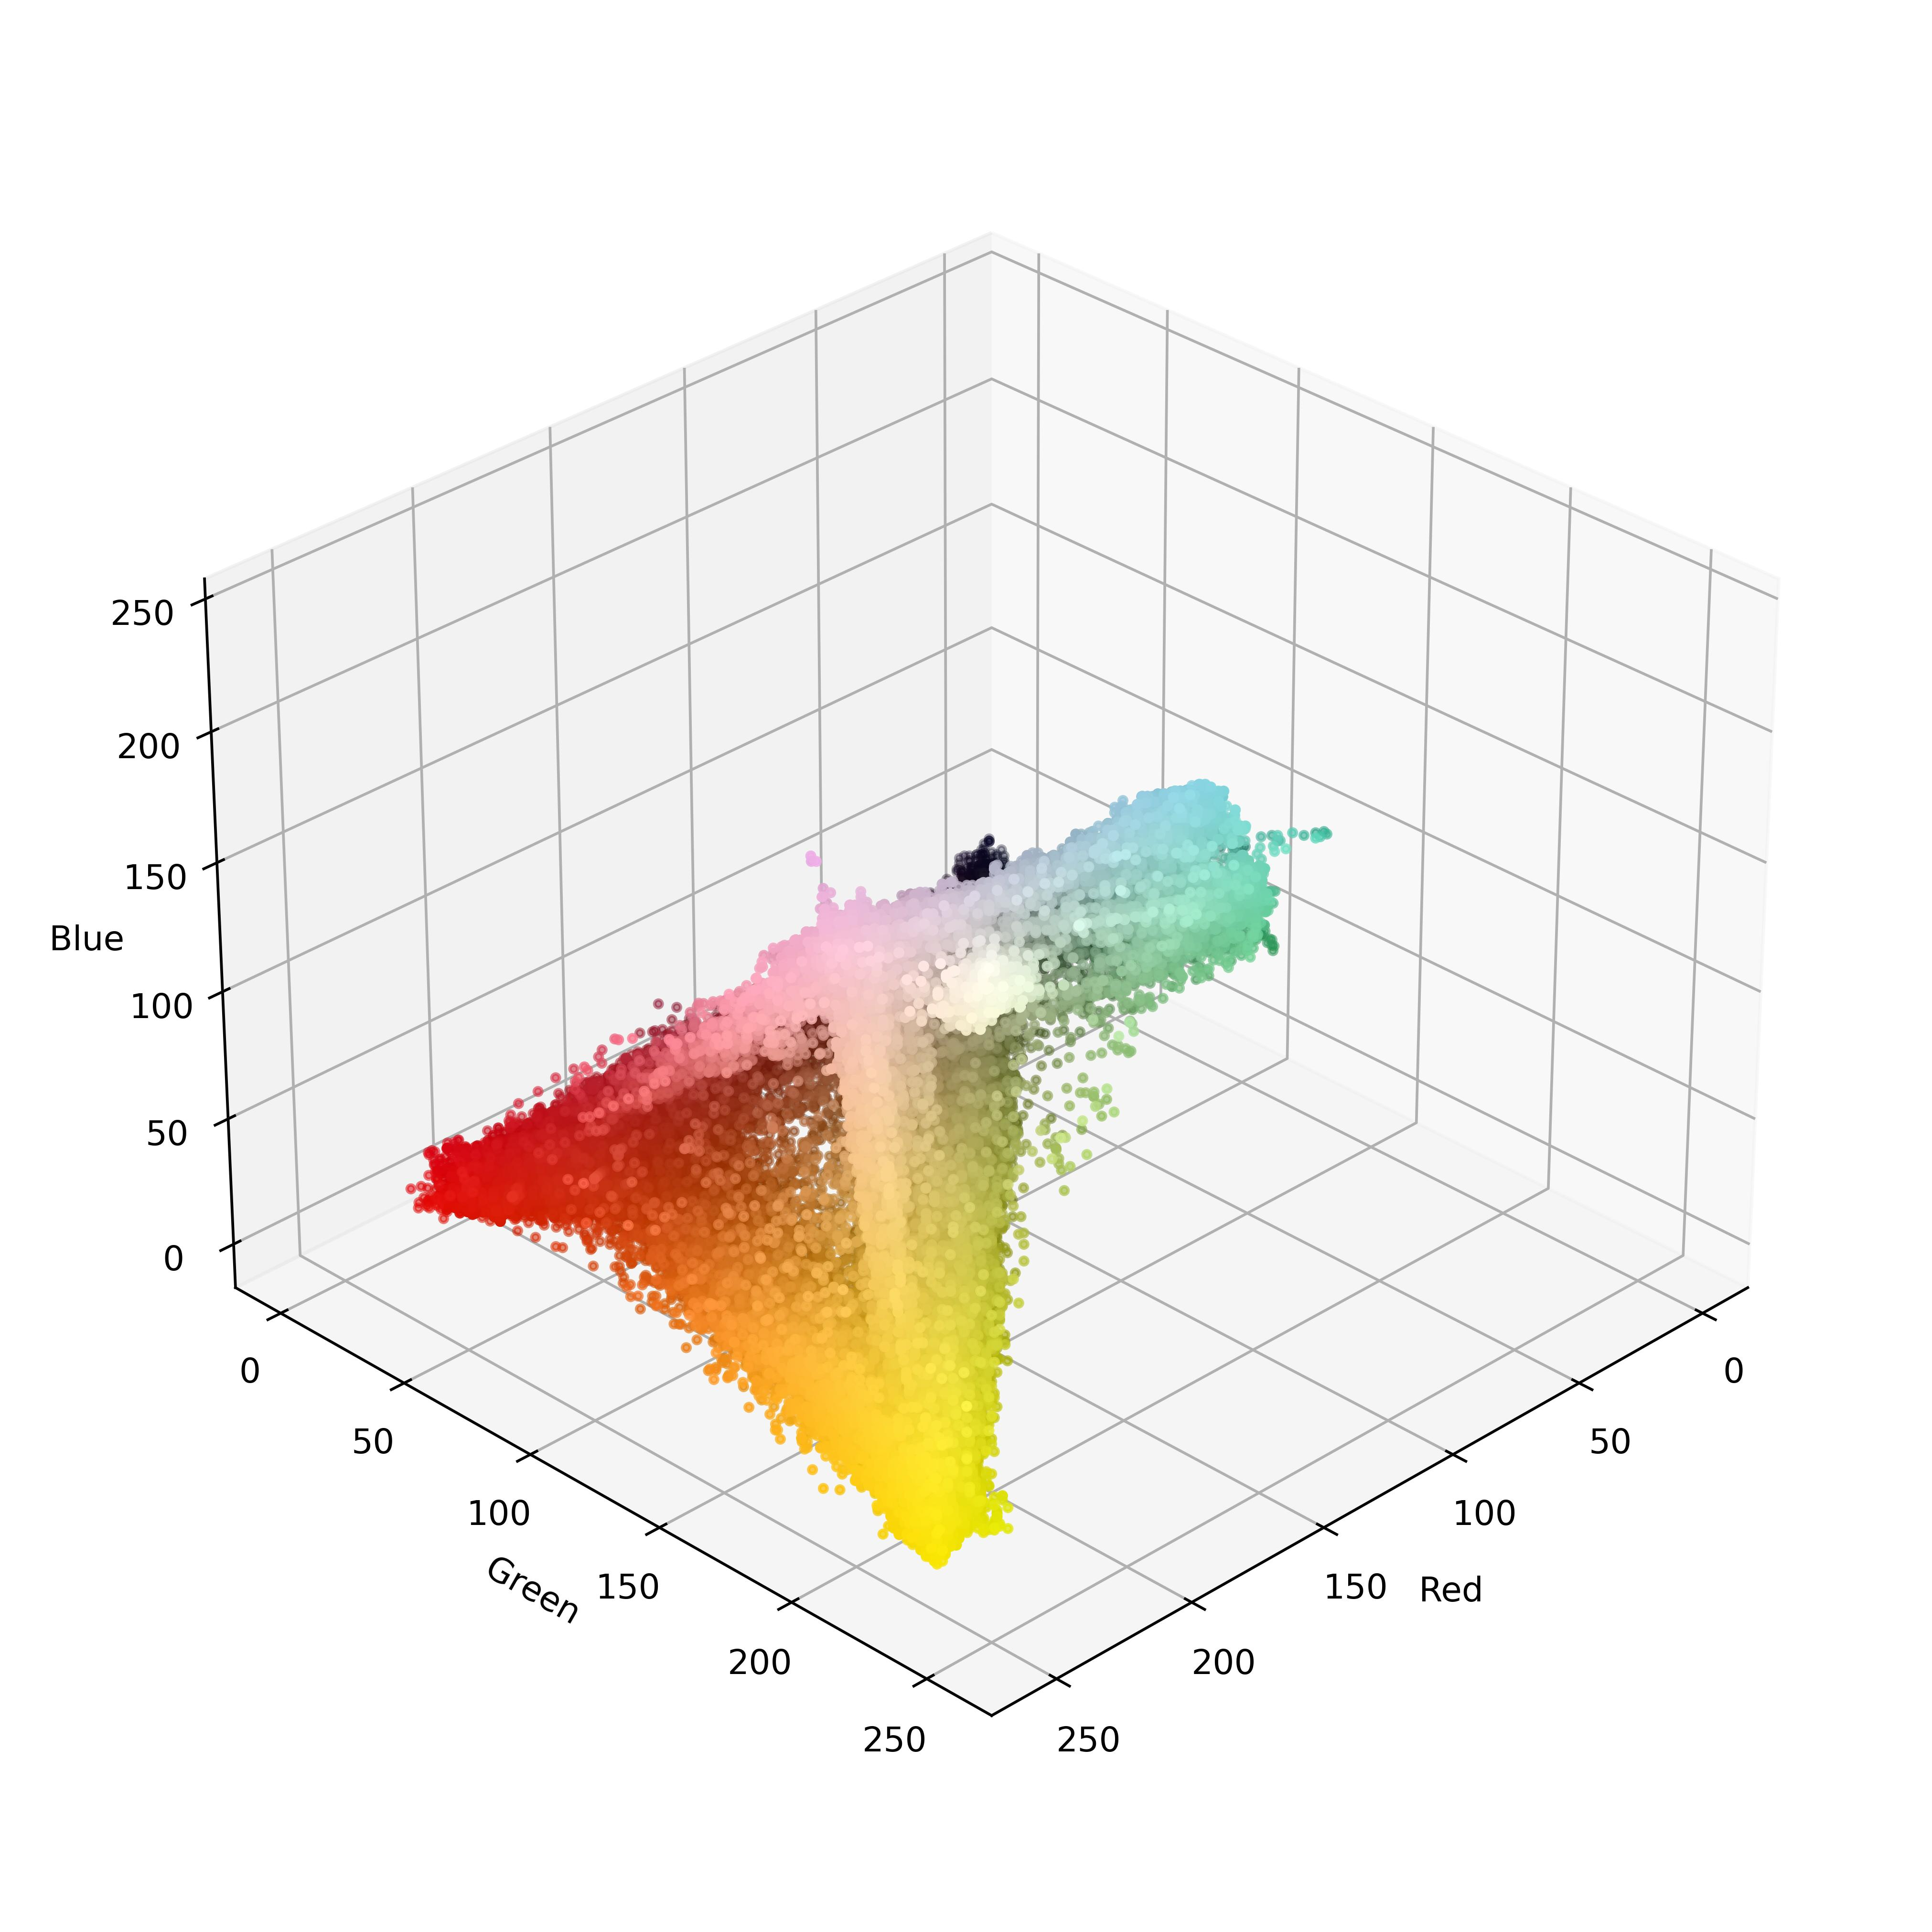
\includegraphics[width=\textwidth]{main_files/figure-latex/4_5_red_marilyn_original_scatter.jpg}
    \caption{Red Marilyn RGB Space - 30 \degree elevation, 45 \degree azimuth}
    \label{fig:4_5_red_marilyn_original_scatter}
  \end{subfigure}
  \hfill
  \begin{subfigure}{0.45\textwidth}
    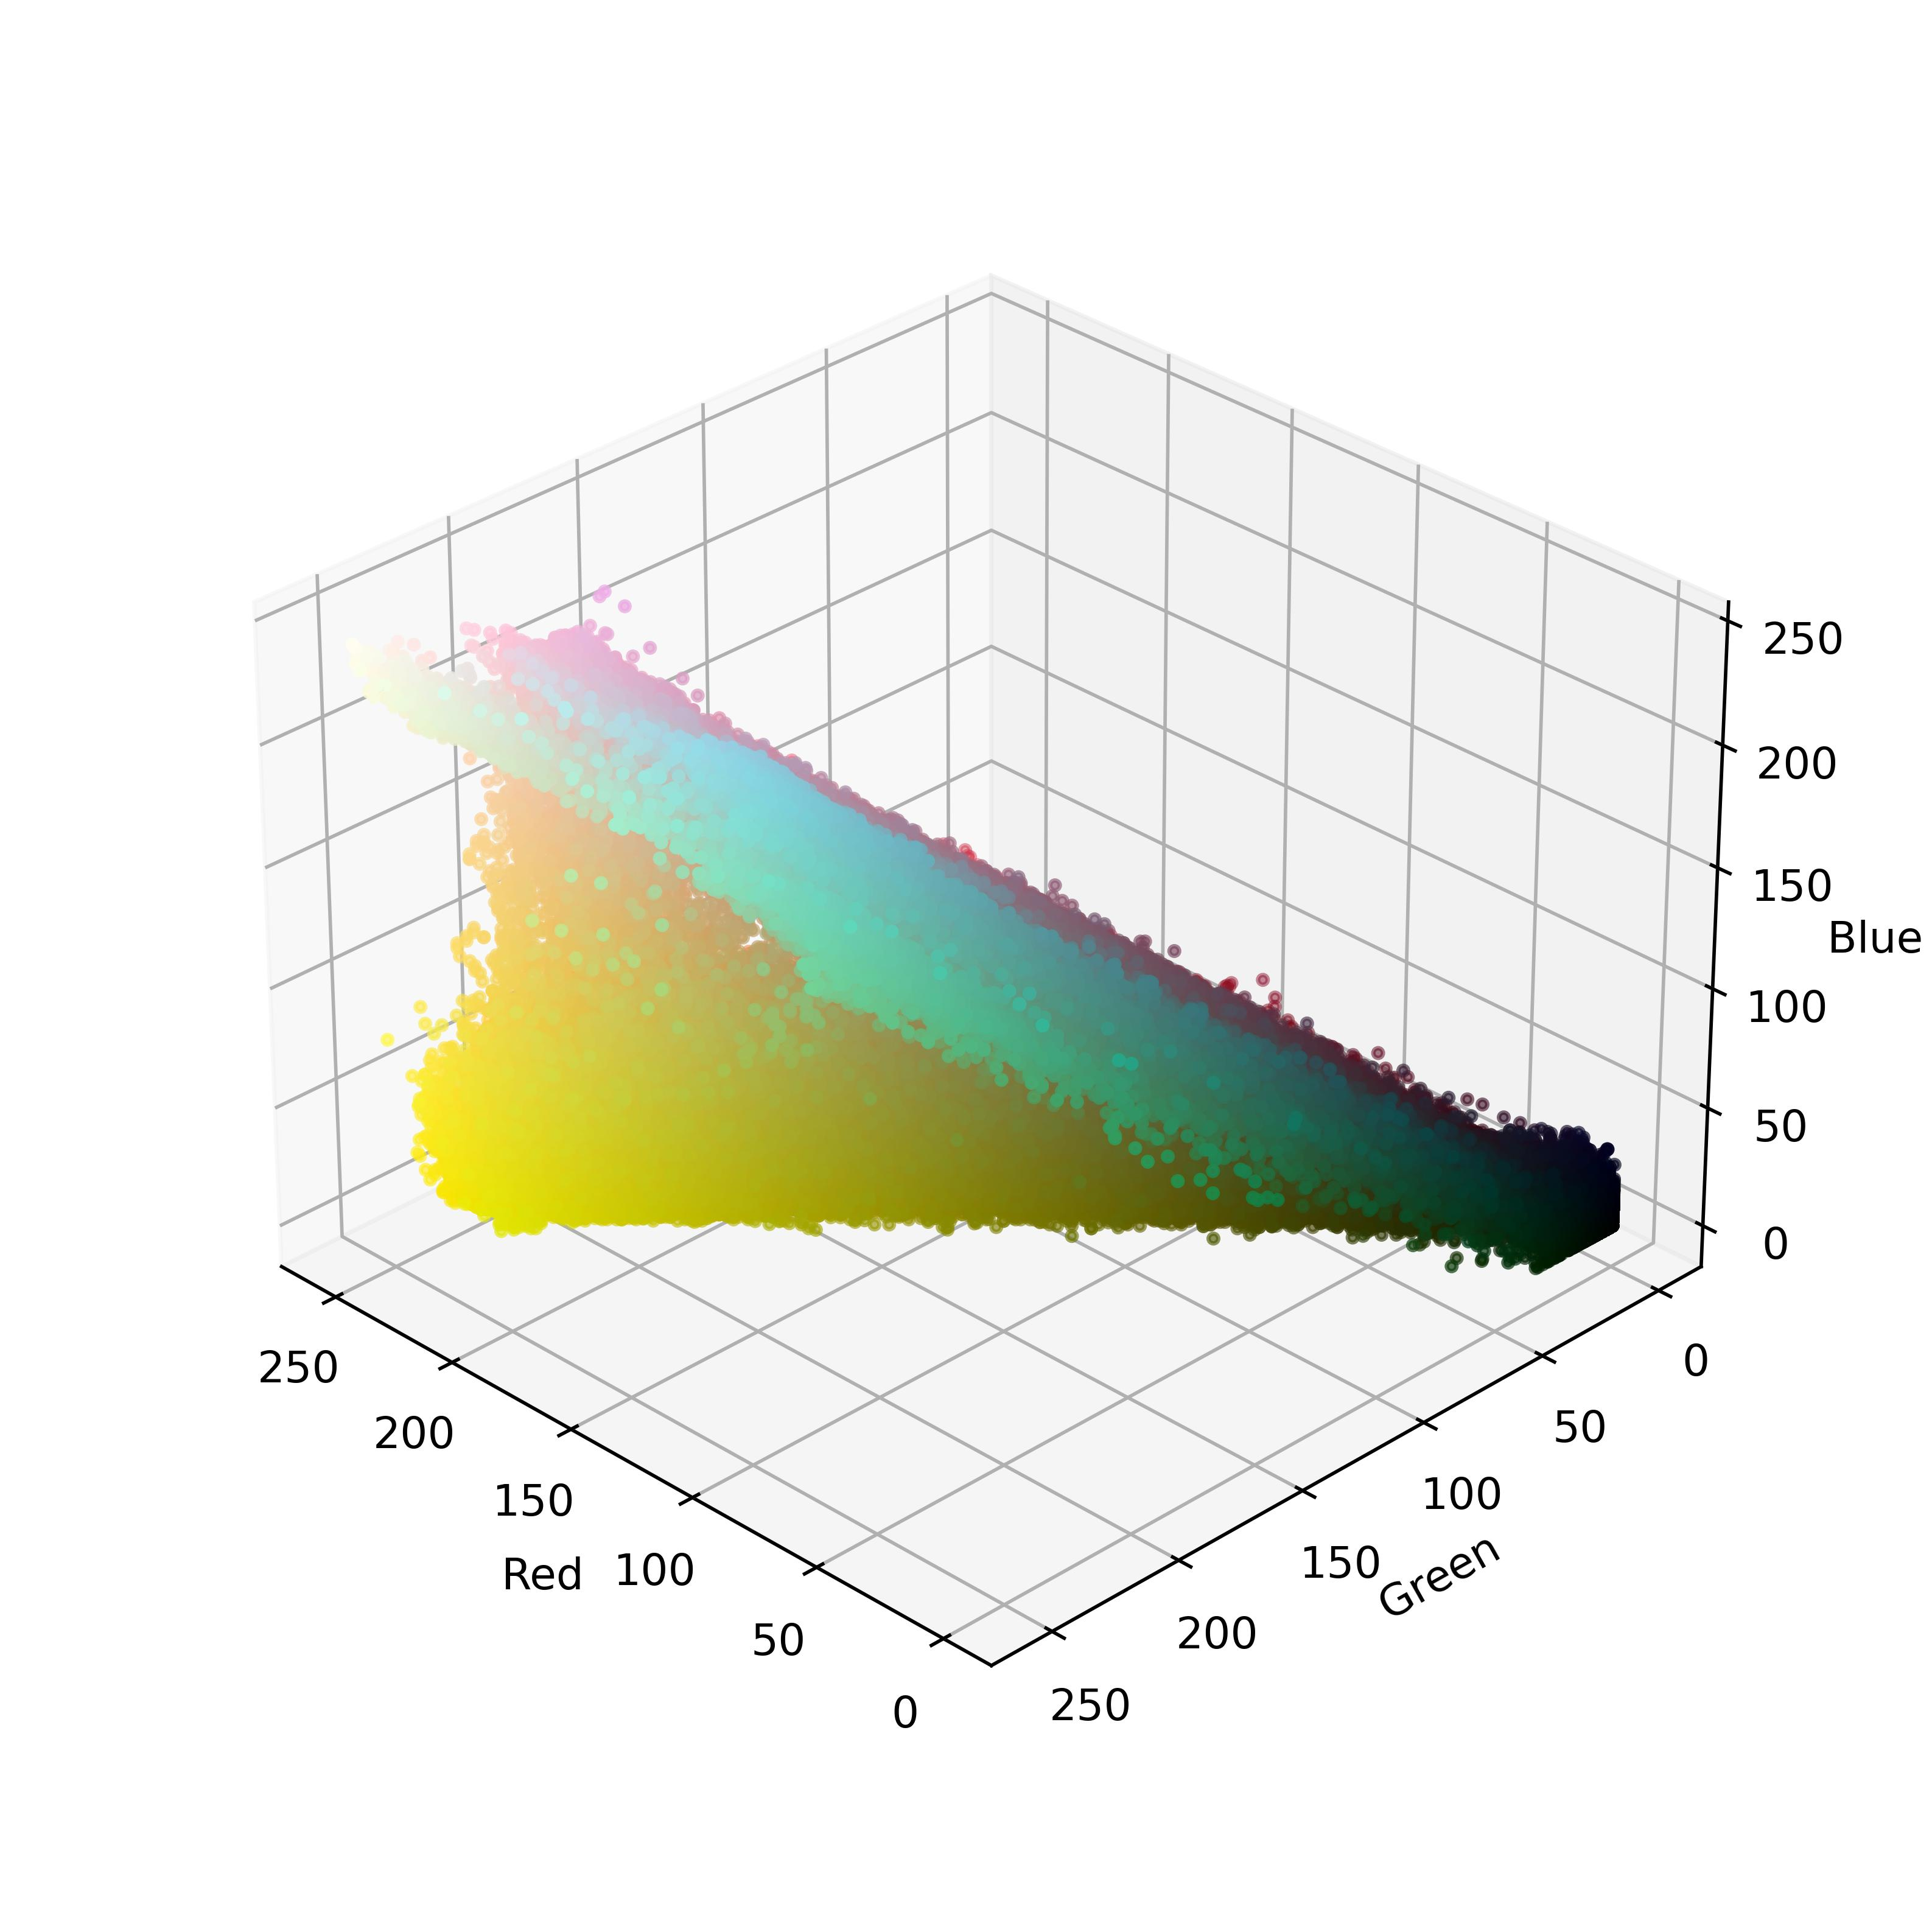
\includegraphics[width=\textwidth]{main_files/figure-latex/4_6_red_marilyn_original_scatter.jpg}
    \caption{Red Marilyn RGB Space - 30 \degree elevation, 135 \degree azimuth}
    \label{fig:4_6_red_marilyn_original_scatter}
  \end{subfigure}
  \label{fig:red_marilyn_original_scatter_1}
\end{figure}

\begin{figure}[ht]\ContinuedFloat
  \centering
  \begin{subfigure}{0.45\textwidth}
    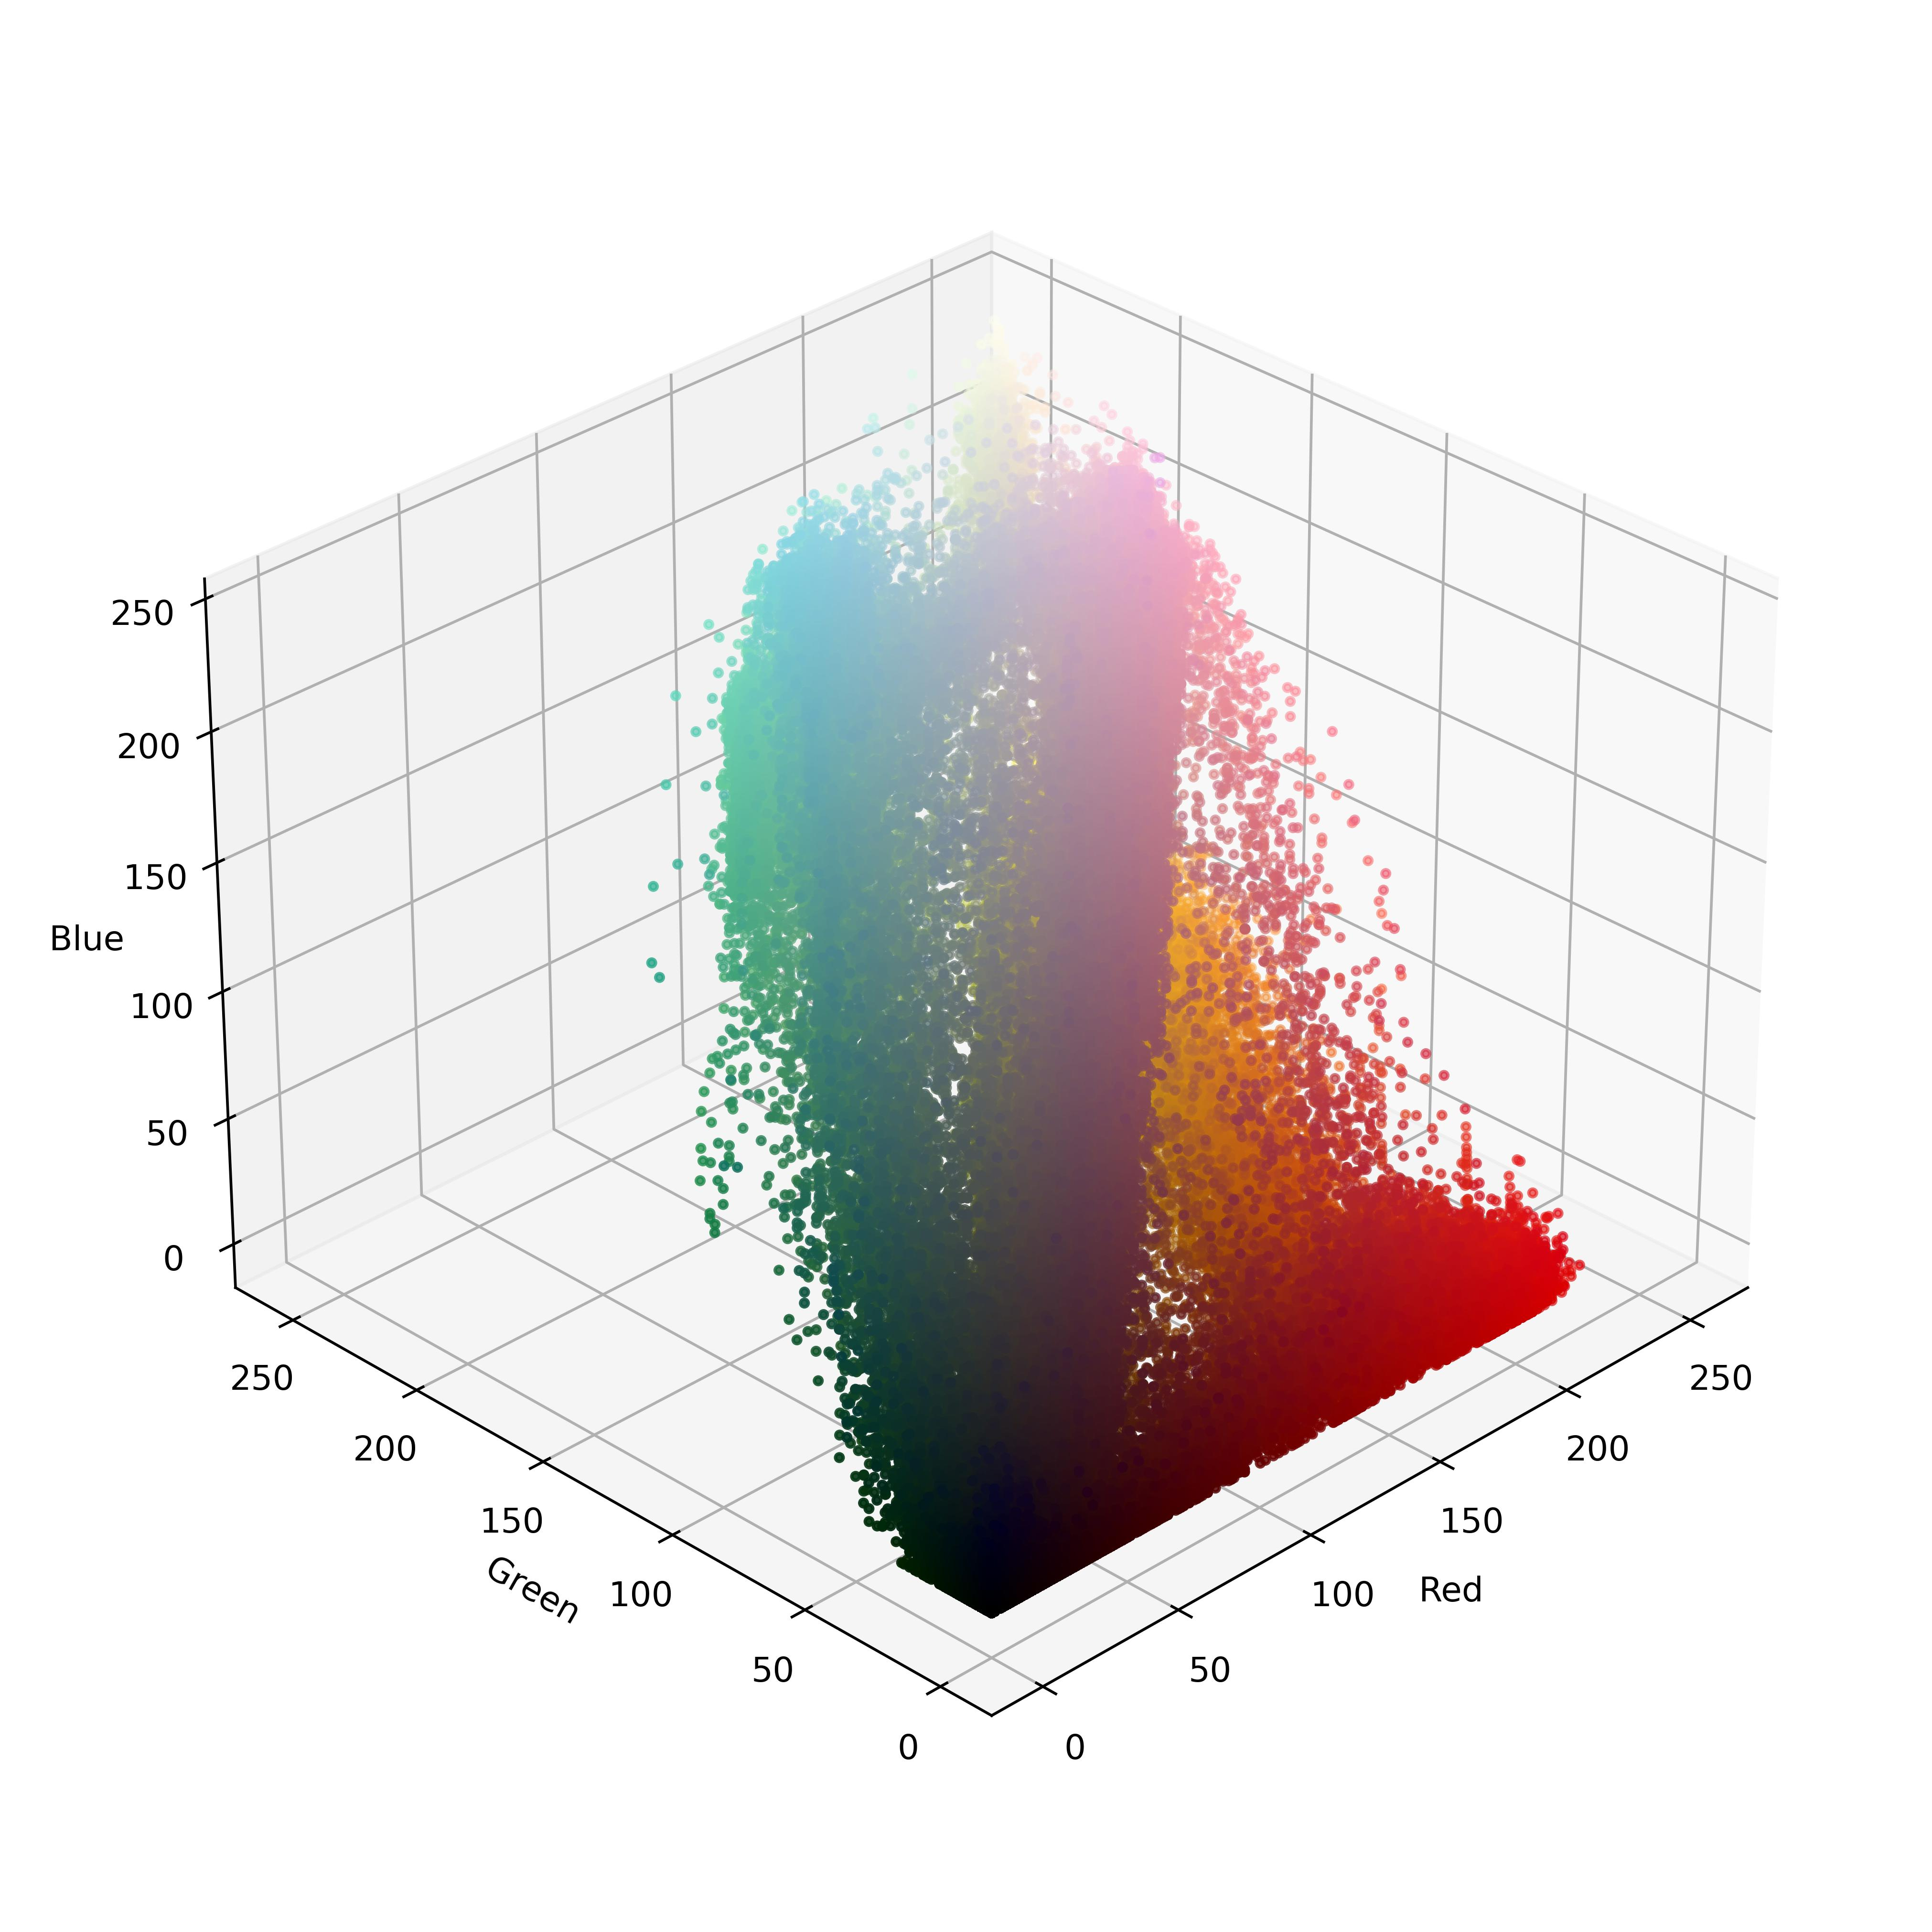
\includegraphics[width=\textwidth]{main_files/figure-latex/4_7_red_marilyn_original_scatter.jpg}
    \caption{Red Marilyn RGB Space - 30 \degree elevation, 225 \degree azimuth}
    \label{fig:4_7_red_marilyn_original_scatter}
  \end{subfigure}
  \hfill
  \begin{subfigure}{0.45\textwidth}
    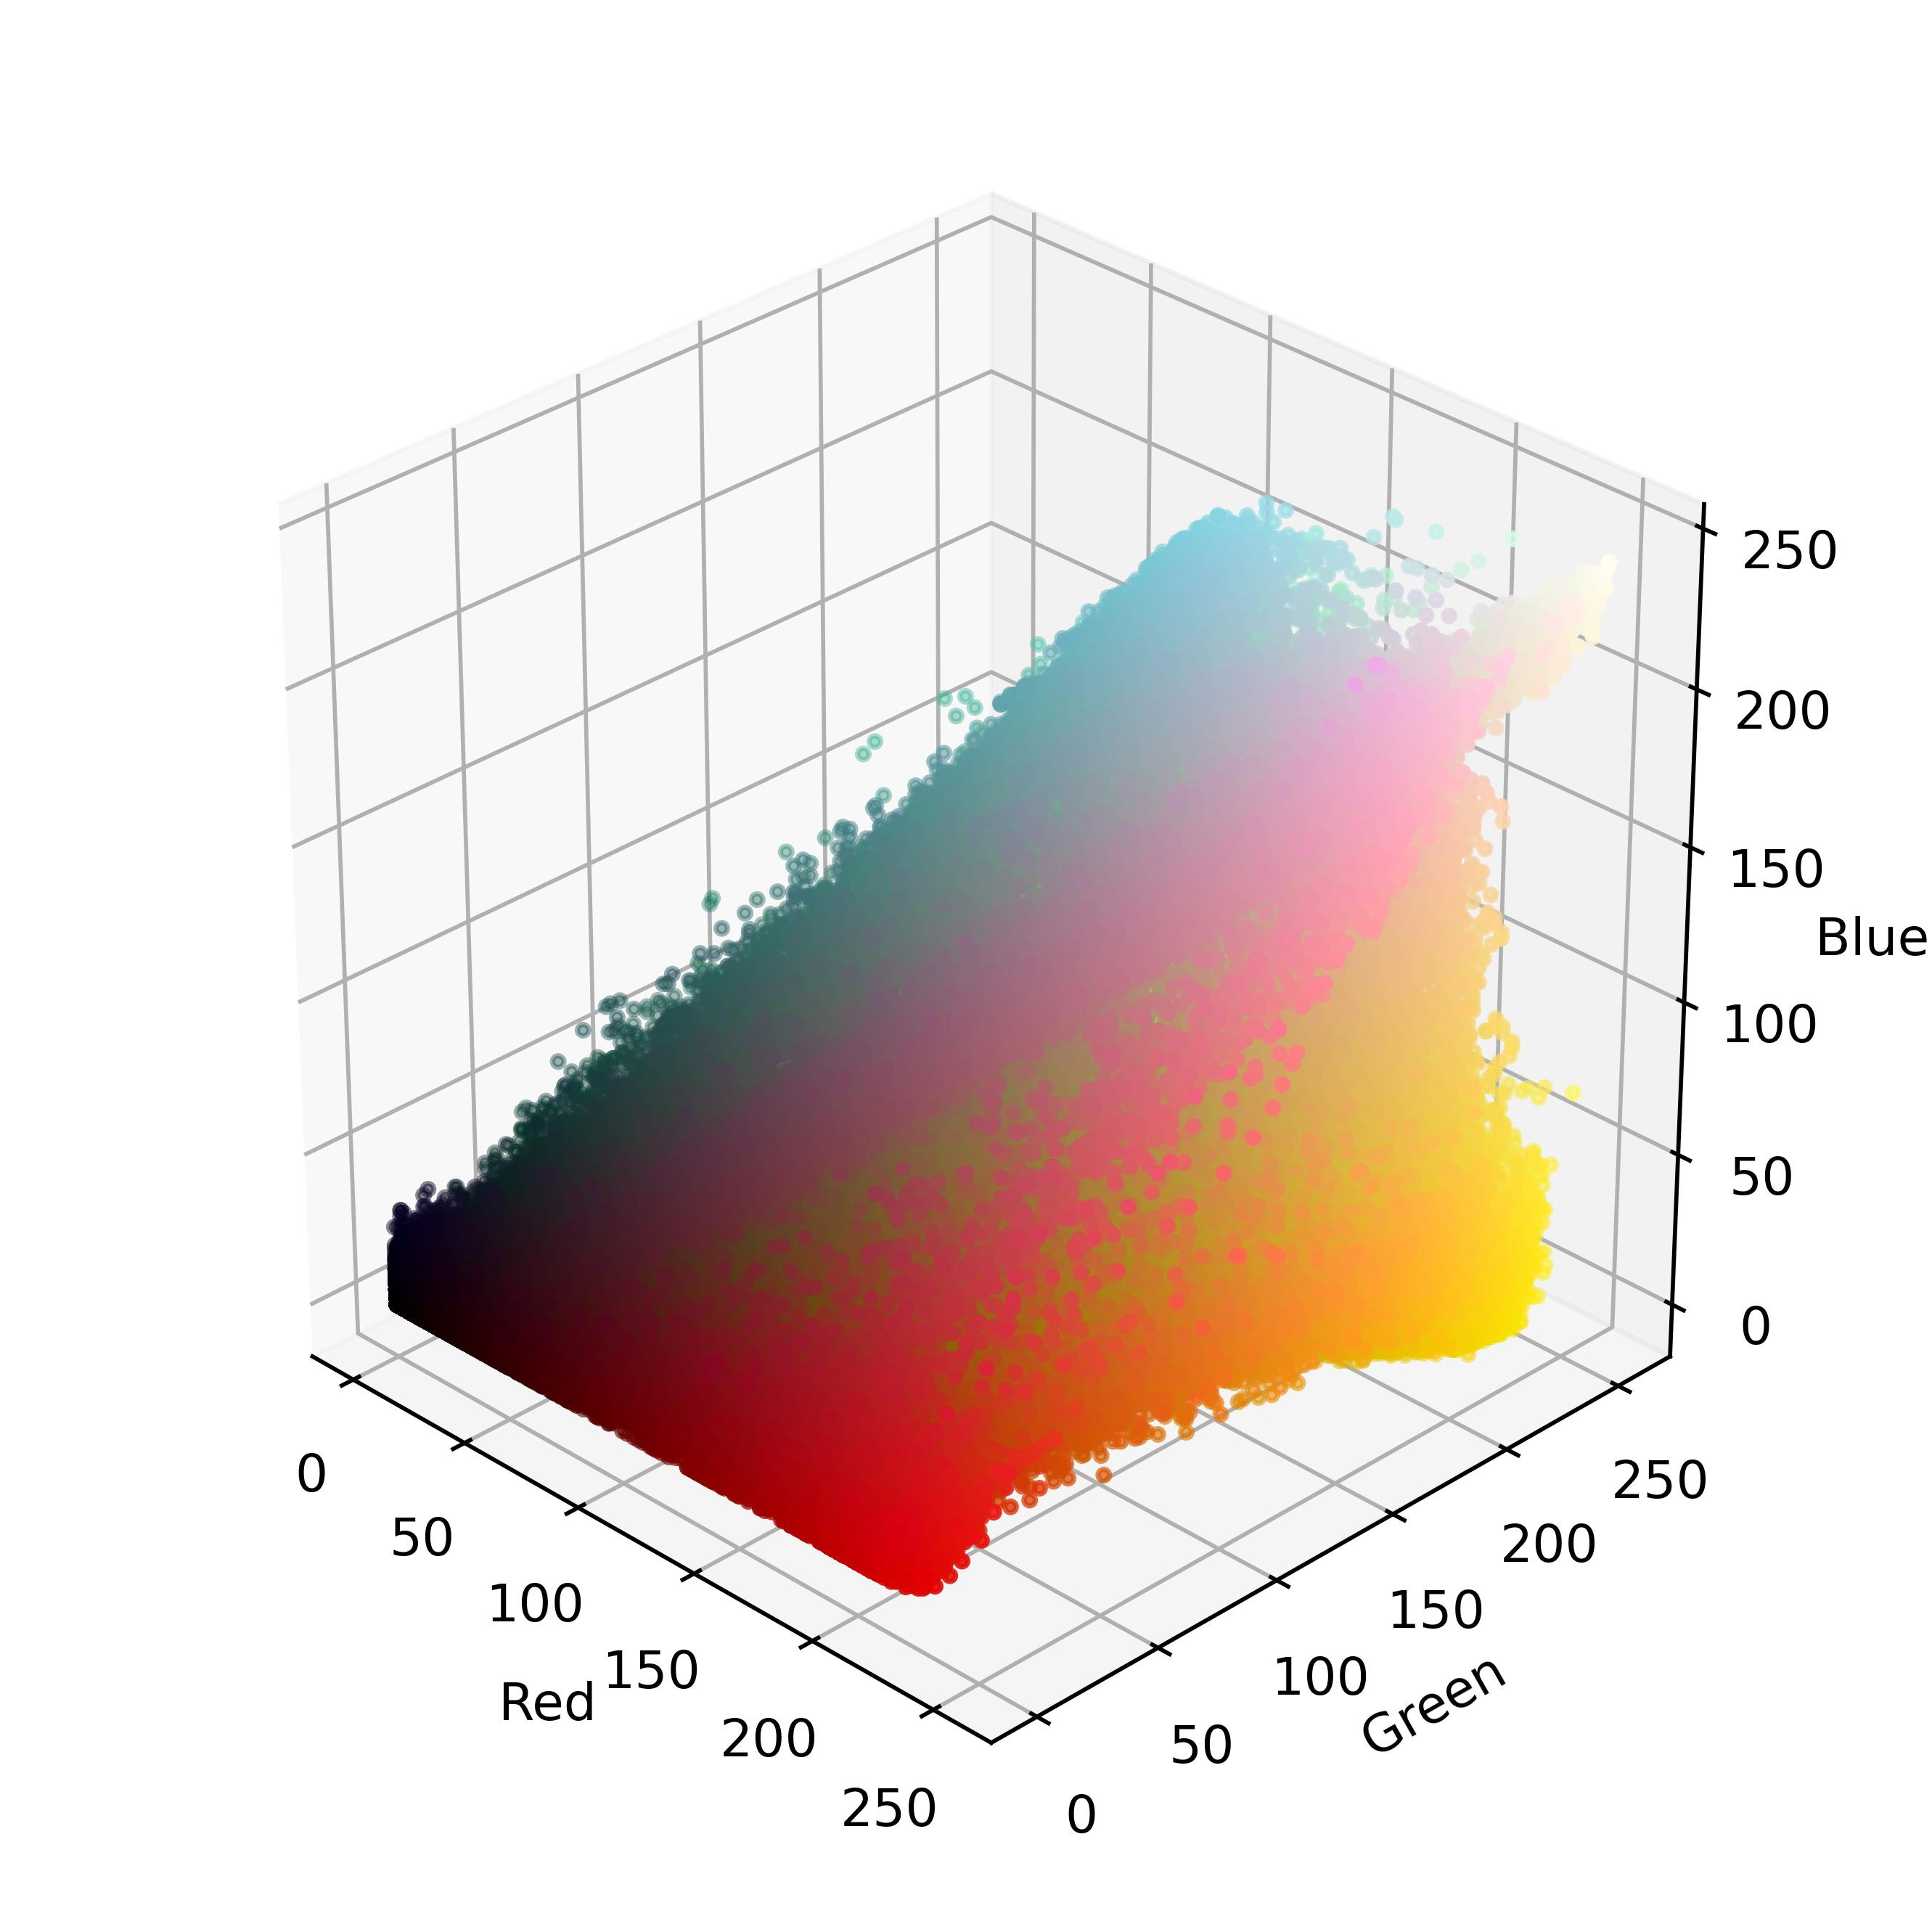
\includegraphics[width=\textwidth]{main_files/figure-latex/4_8_red_marilyn_original_scatter.jpg}
    \caption{Red Marilyn RGB Space - 30 \degree elevation, 315 \degree azimuth}
    \label{fig:4_8_red_marilyn_original_scatter}
  \end{subfigure}
  \caption{The RGB space occupied by the pixels for the entire image of Red Marilyn, showing different angles: (a) 30 \degree elevation, 45 \degree azimuth, (b) 30 \degree elevation, 135 \degree azimuth, (c) 30 \degree elevation, 225 \degree azimuth, (d) 30 \degree elevation, 315 \degree azimuth. These variations highlight the color distribution within the artwork.}
  \label{fig:red_marilyn_original_scatter_2}
\end{figure}

Figure 5 displays the RGB space of ``Red Marilyn'' from four different
angles. In (a), the density of pixels representing different parts of
the image is shown, revealing a balanced mix of colors including a red
background, yellow hair, pink cheeks, and blue eye shades. The shape of
the 3D scatter plot in (a) indicates a broad, dispersed distribution of
colors, showing the diverse color use in the background and facial
features.

In (b), the plot illustrates how colors are distributed from darker
pixels at the bottom to brighter pixels at the top, highlighting shading
gradients. This gradient reflects the shading around Marilyn's clothes,
eye shades, and hair, adding depth to the portrait. The darker pixels
likely represent shadows in the hair and facial contours, while the
brighter pixels correspond to highlights on her clothes and hair. The
shape in (b) is elongated, showing a clear separation between the dark
and bright areas.

In (c), the concentration of the brightest pixels is evident, showing
specific groupings likely related to prominent features. This highlights
the intense colors used in Marilyn's lips, eye shades, clothes, and
other facial highlights. The plot suggests a focused clustering of
bright colors, indicating areas where Warhol applied more vivid hues to
draw attention. The shape in (c) suggests a dense clustering of bright
colors.

In (d), the color distribution from dark to light is presented from a
different angle, allowing us to observe the distribution of colors in
areas such as hair and eye shades with dense red on the bottom from the
background. The shapes in (b) through (d) all reflect a similar
elongated form as seen in ``Orange Marilyn,'' but with a more spread-out
appearance, resembling a long and thick funnel. This shape shows a clear
gradient from dark to light colors, indicating that the colors are
brighter, bolder, and more impactful than in ``Orange Marilyn.'' This
consistent shape across different angles highlights the structured way
Warhol applied color to create depth and contrast in the ``Red Marilyn''
painting.

\begin{figure}[ht]
  \centering
  \begin{subfigure}{0.45\textwidth}
    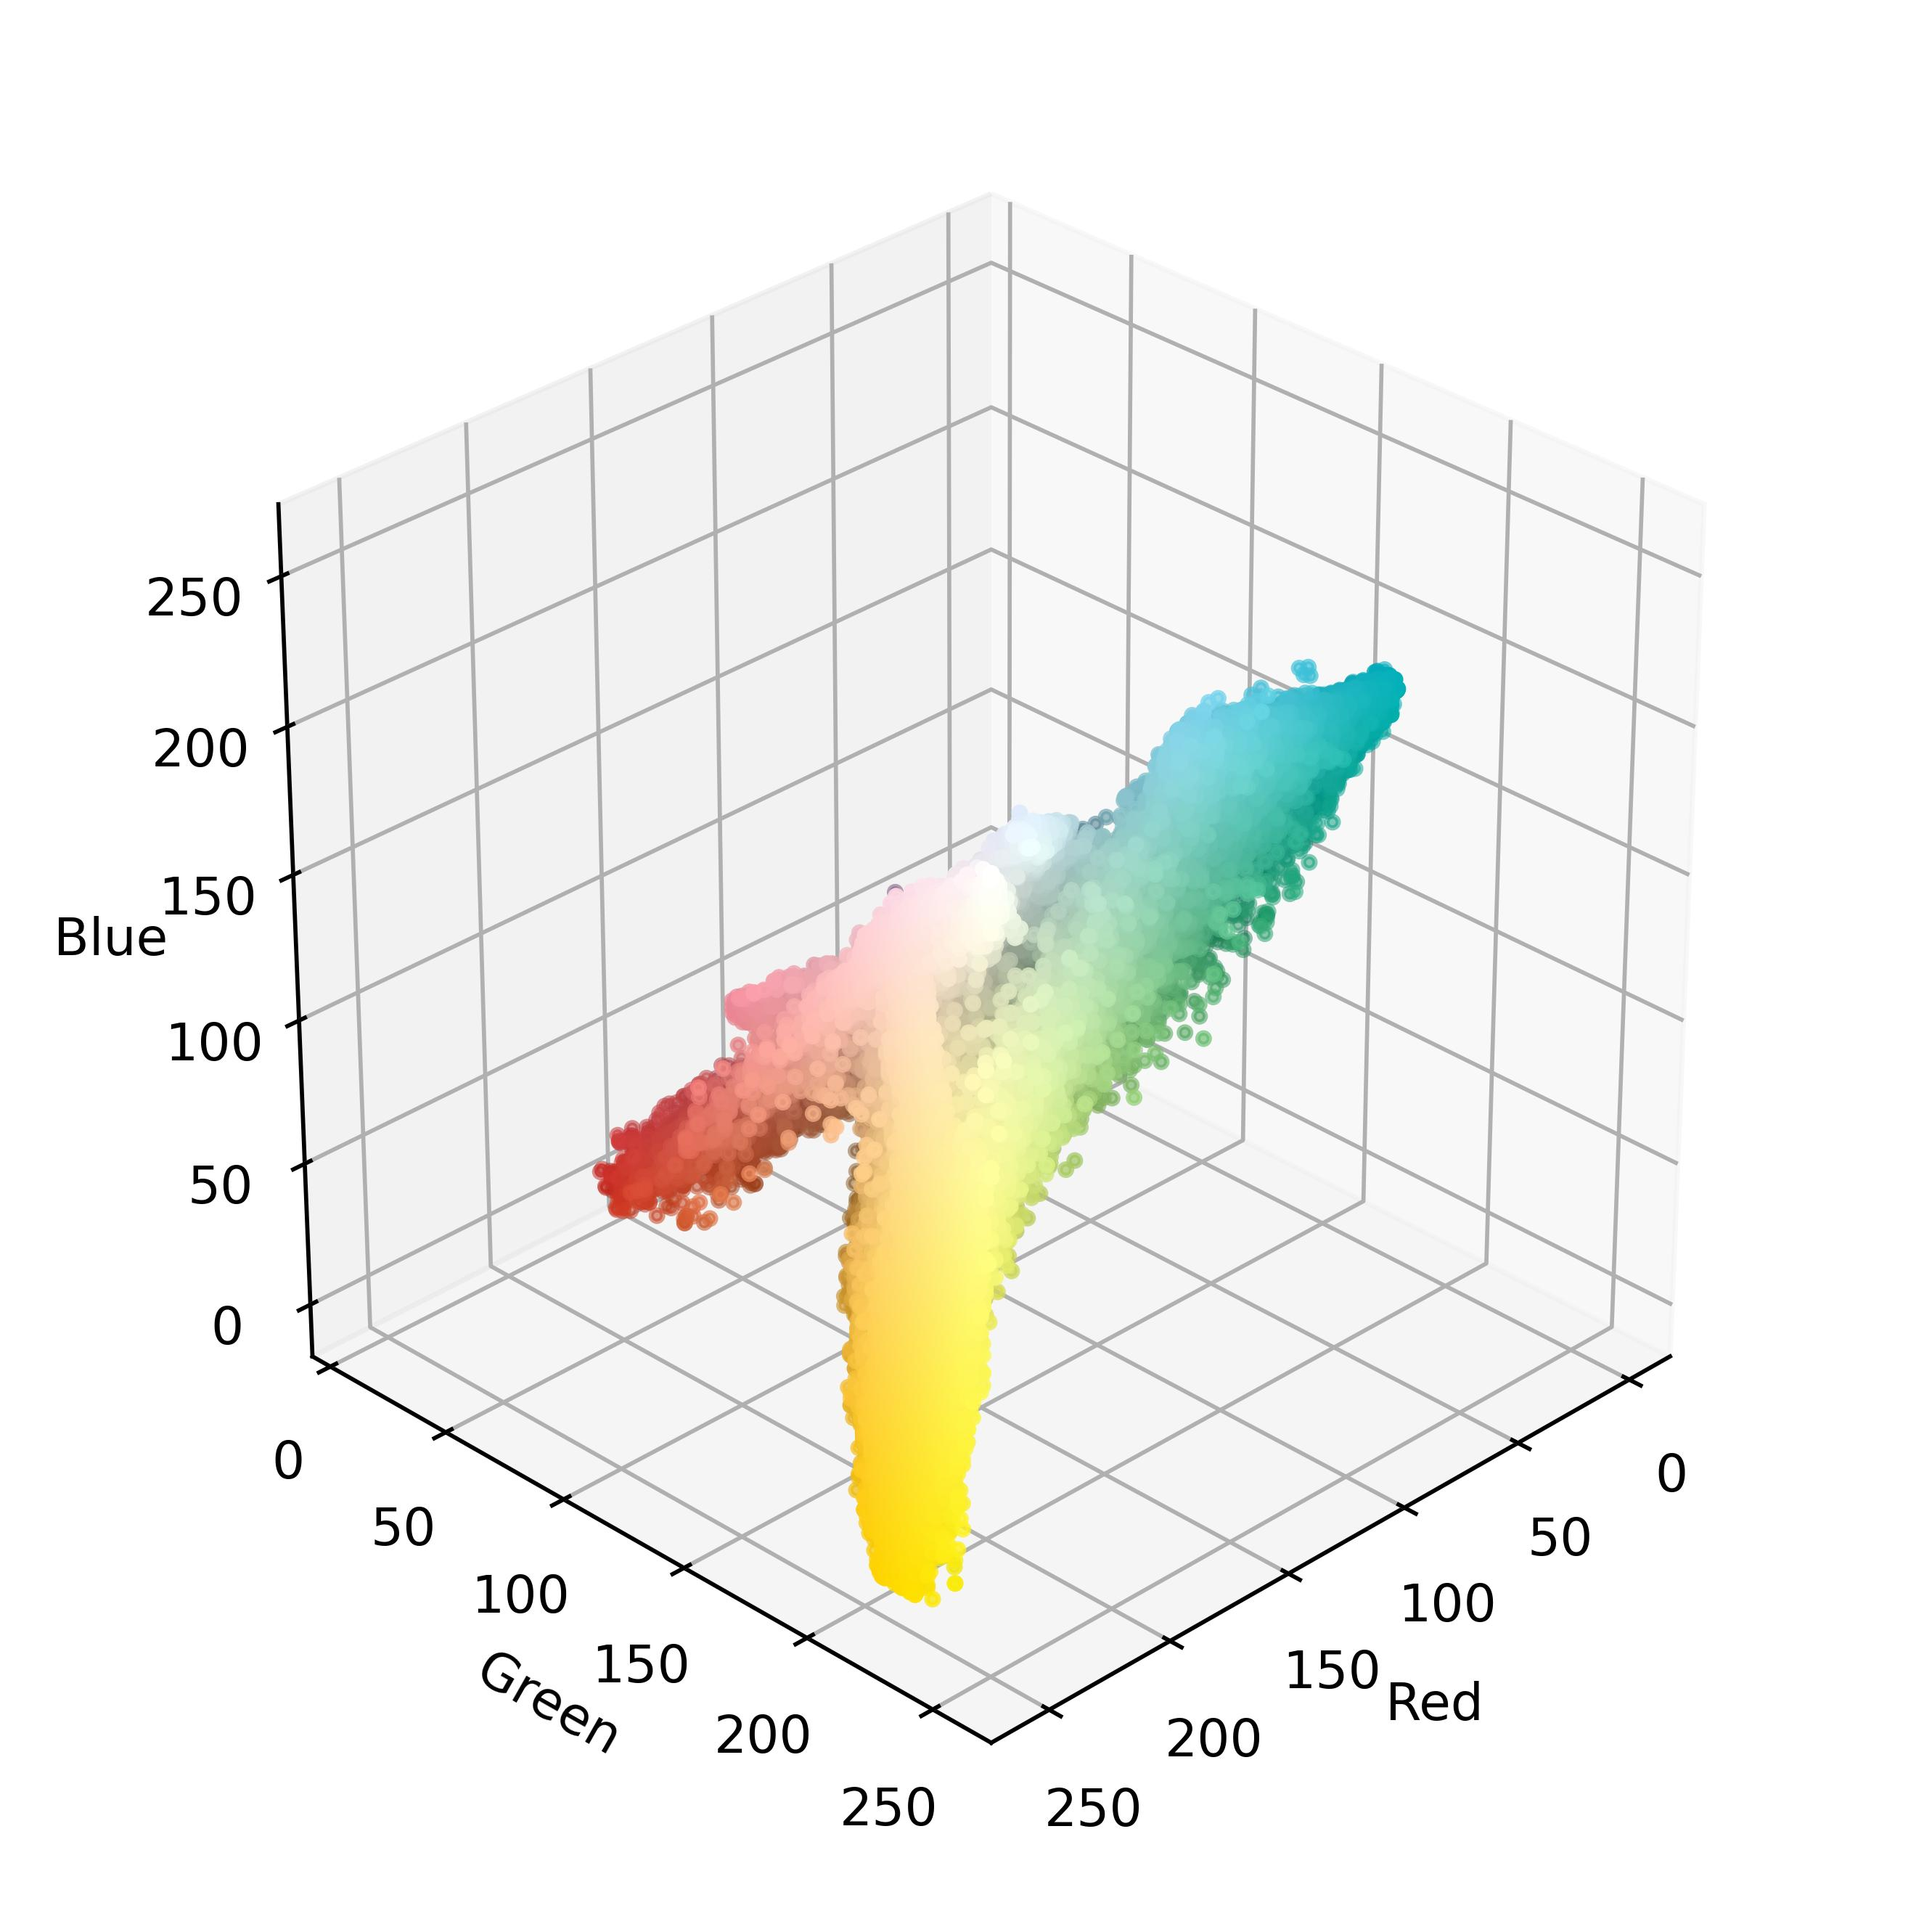
\includegraphics[width=\textwidth]{main_files/figure-latex/4_9_turq_marilyn_original_scatter.jpg}
    \caption{Turquoise Marilyn RGB Space - 30 \degree elevation, 45 \degree azimuth}
    \label{fig:4_9_turq_marilyn_original_scatter}
  \end{subfigure}
  \hfill
  \begin{subfigure}{0.45\textwidth}
    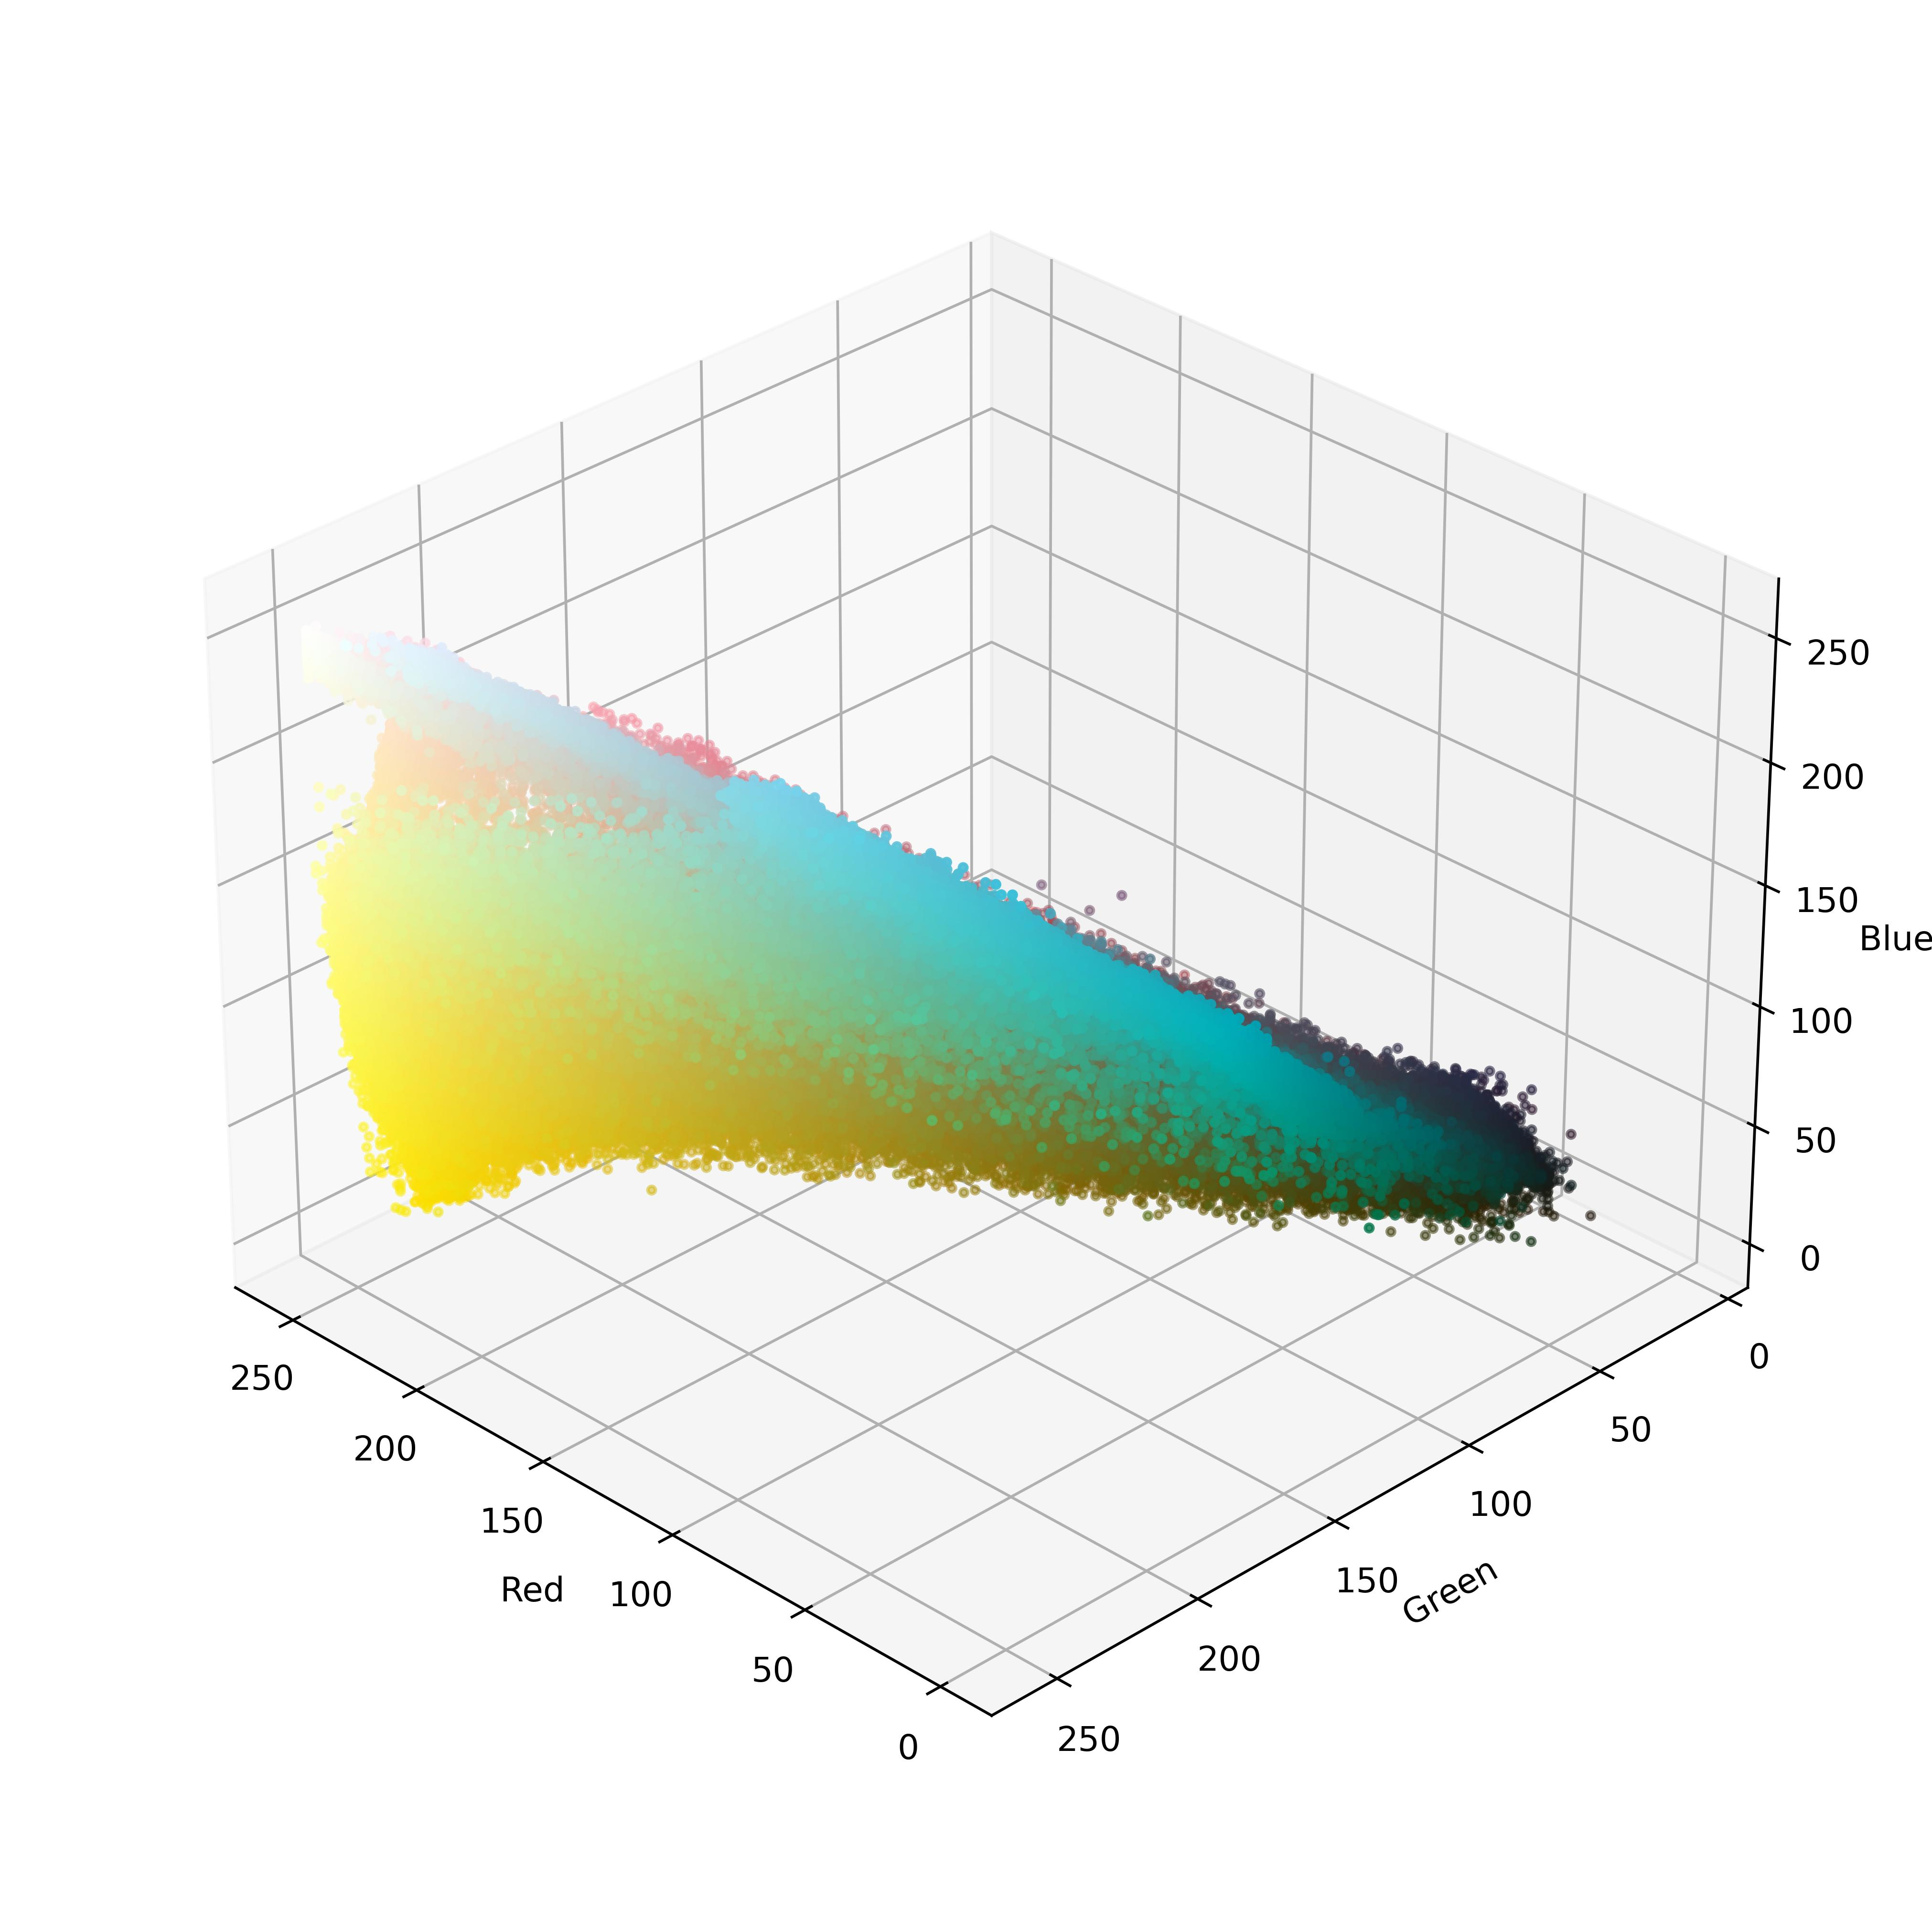
\includegraphics[width=\textwidth]{main_files/figure-latex/4_10_turq_marilyn_original_scatter.jpg}
    \caption{Turquoise Marilyn RGB Space - 30 \degree elevation, 135 \degree azimuth}
    \label{fig:4_10_turq_marilyn_original_scatter}
  \end{subfigure}
  \label{fig:turq_marilyn_original_scatter_1}
\end{figure}

\begin{figure}[ht]\ContinuedFloat
  \centering
  \begin{subfigure}{0.45\textwidth}
    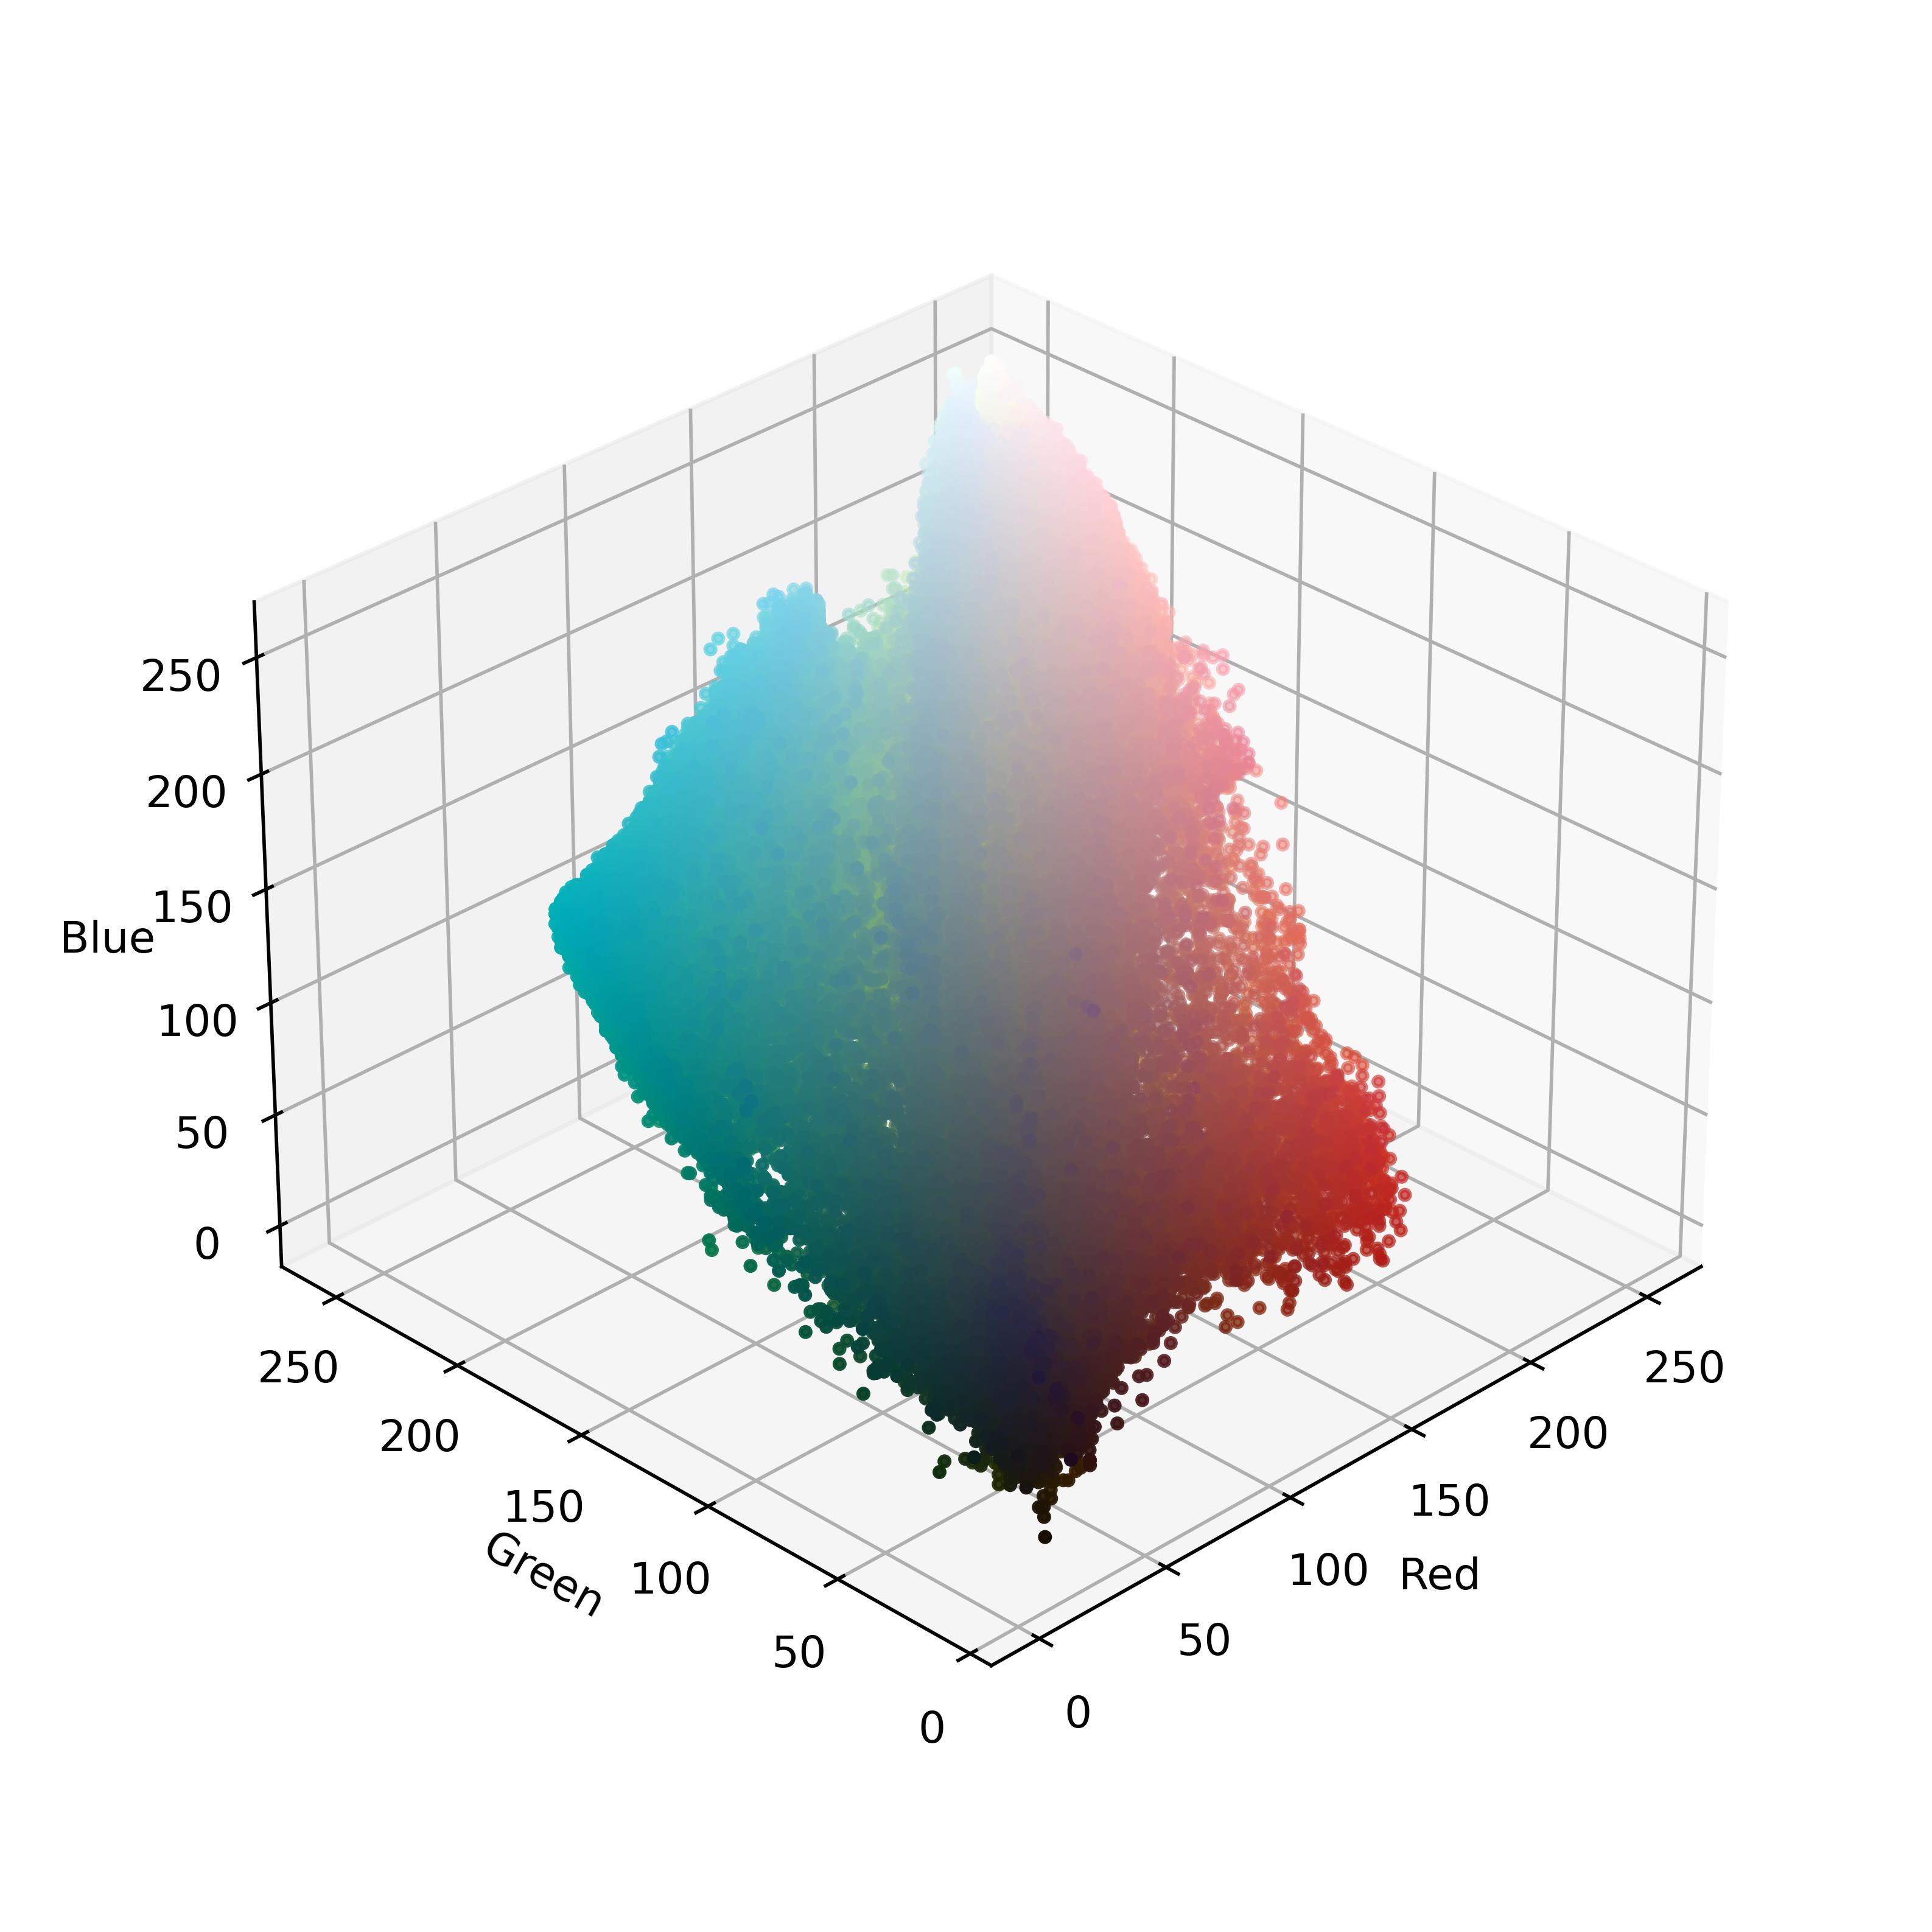
\includegraphics[width=\textwidth]{main_files/figure-latex/4_11_turq_marilyn_original_scatter.jpg}
    \caption{Turquoise Marilyn RGB Space - 30 \degree elevation, 225 \degree azimuth}
    \label{fig:4_11_turq_marilyn_original_scatter}
  \end{subfigure}
  \hfill
  \begin{subfigure}{0.45\textwidth}
    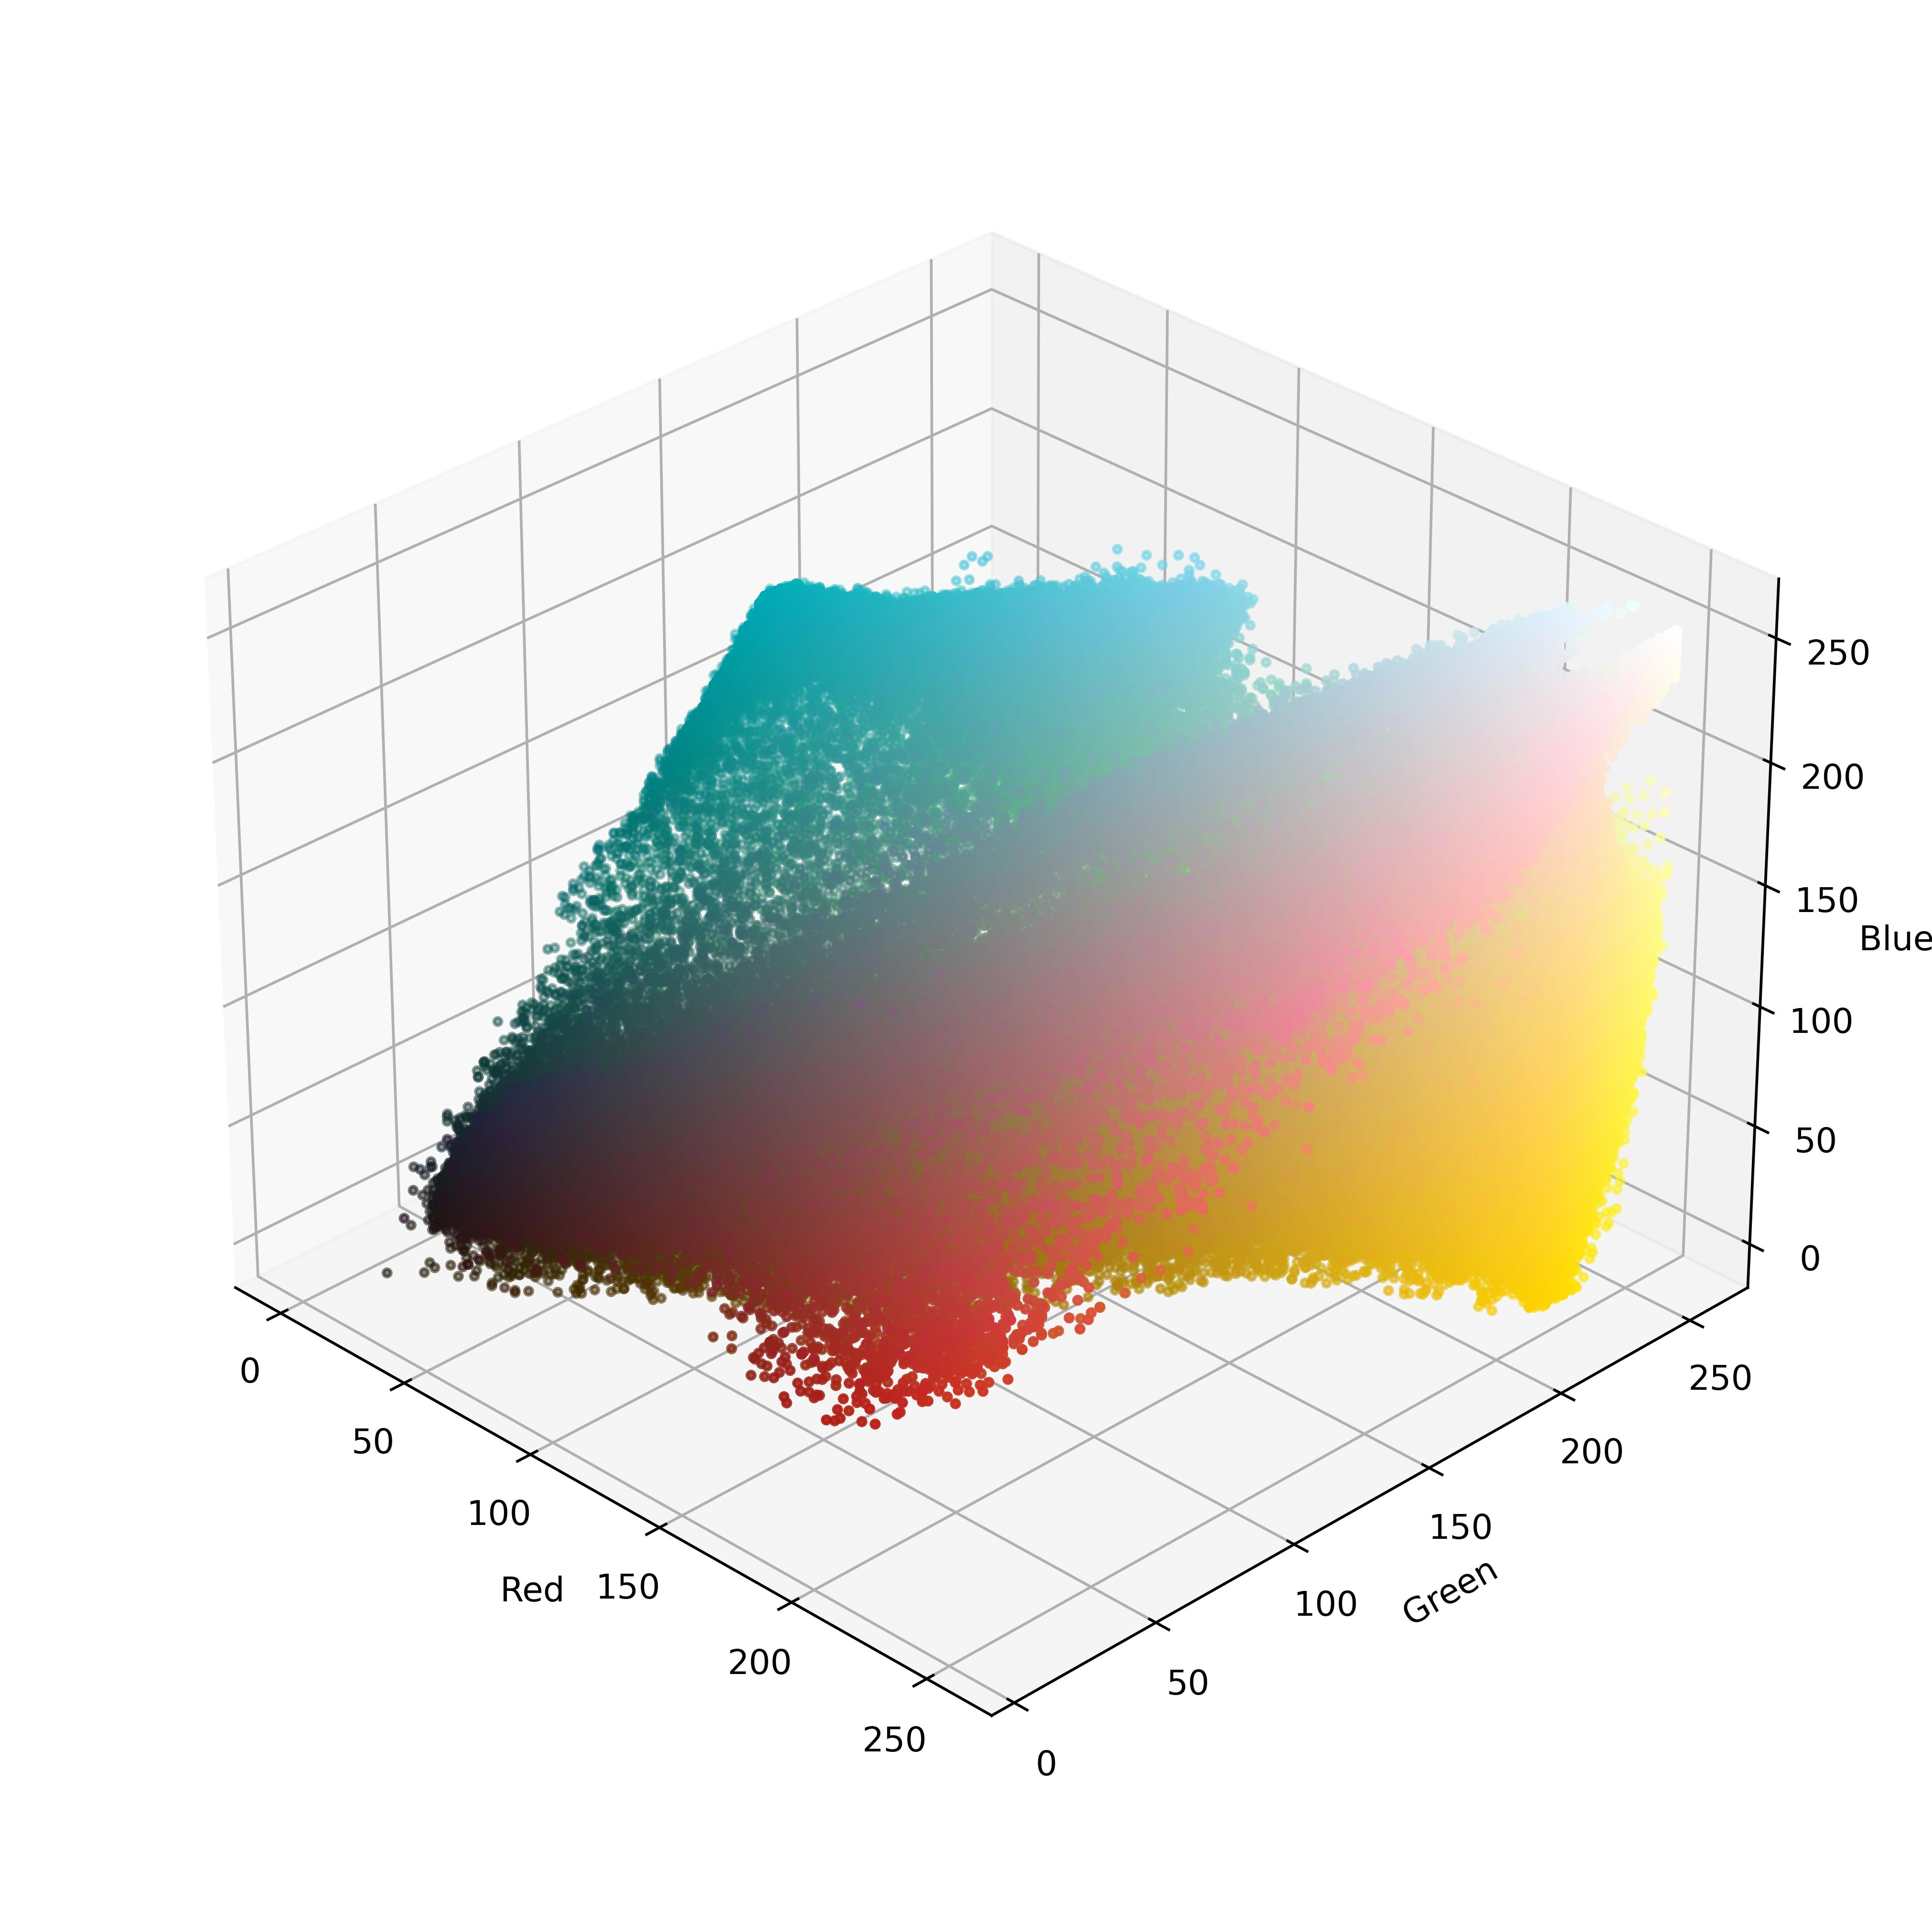
\includegraphics[width=\textwidth]{main_files/figure-latex/4_12_turq_marilyn_original_scatter.jpg}
    \caption{Turquoise Marilyn RGB Space - 30 \degree elevation, 315 \degree azimuth}
    \label{fig:4_12_turq_marilyn_original_scatter}
  \end{subfigure}
  \caption{The RGB space occupied by the pixels for the entire image of Turquoise Marilyn, showing different angles: (a) 30 \degree elevation, 45 \degree azimuth, (b) 30 \degree elevation, 135 \degree azimuth, (c) 30 \degree elevation, 225 \degree azimuth, (d) 30 \degree elevation, 315 \degree azimuth. These variations highlight the color distribution within the artwork.}
  \label{fig:turq_marilyn_original_scatter_2}
\end{figure}

Figure 6 displays the RGB space of ``Turquoise Marilyn'' from four
different angles.

In (a), the density of pixels shows a broad mix of colors including
turquoise, yellow, pink, and red, which correspond to the background,
hair, face, and lips of the painting. The shape of the 3D scatter plot
indicates a dispersed distribution of colors, reflecting the varied
color use throughout the image. Most pixels cluster in the turquoise
region, which is the background color of this painting, extending in
three directions.

In (b), the distribution of colors transitions from darker pixels at the
bottom to brighter pixels at the top, highlighting the gradient in
shading. This transition illustrates the shading around Marilyn's facial
features and hair, adding depth to the portrait. The shape shows a clear
gradient from dark to bright areas, with darker pixels on the right side
of the 3D space and brighter pixels on the left.

In (c), the plot emphasizes the concentration of the brightest pixels,
showing specific groupings that likely correspond to Marilyn's lips,
eyes, and other highlighted features. This suggests a focused clustering
of bright colors where Warhol applied vivid hues to draw attention. The
shape suggests a dense clustering of bright colors. Viewing the backside
of (a), it reaffirms that the painting contains a significant number of
turquoise pixels.

In (d), the color distribution from dark to light is presented from a
different angle, allowing us to observe how the colors in the hair and
eye shades are distributed, with a notable presence of turquoise pixels
from the background. The shape reflects the backside of (b), with darker
pixels on the left and brighter pixels on the right.

The shapes in (a) through (d) reflect a similar elongated form,
resembling a long and wide funnel, showing a clear gradient from dark to
light colors. This highlights how the colors are brighter, bolder, and
more impactful in ``Turquoise Marilyn,'' emphasizing the structured
application of color by Warhol to create depth and contrast.

\begin{figure}[ht]
  \centering
  \begin{subfigure}{0.45\textwidth}
    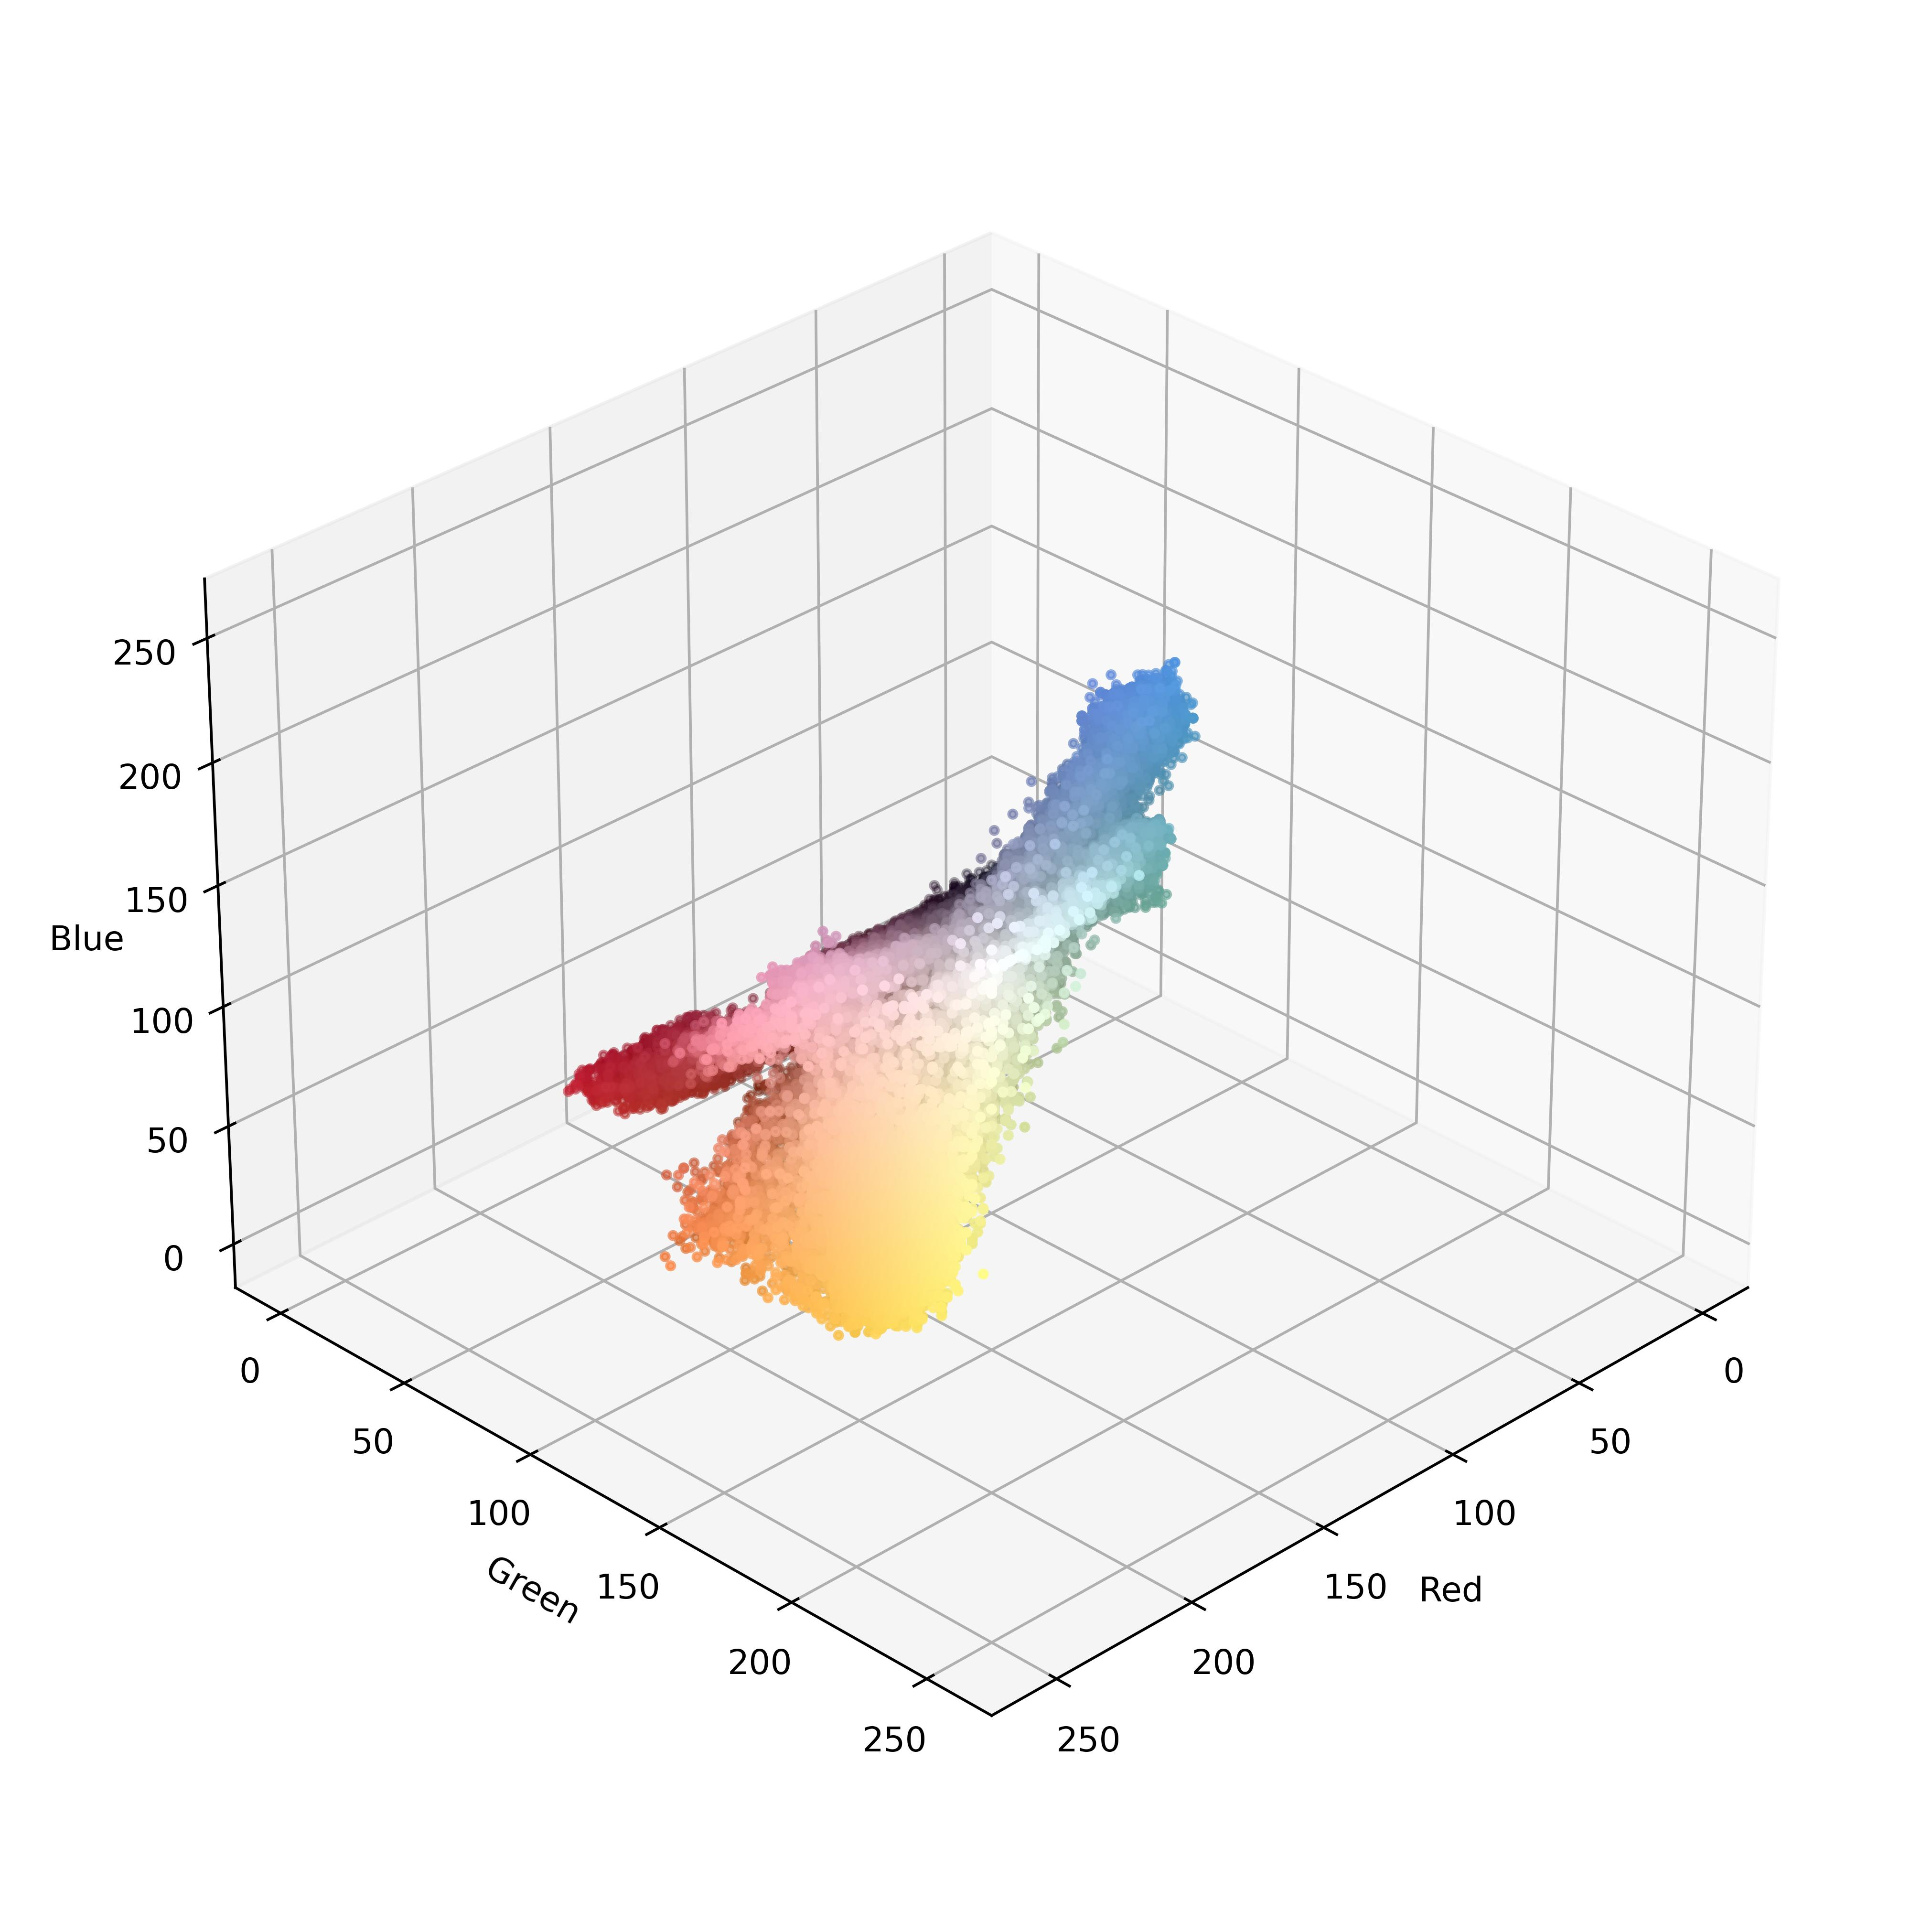
\includegraphics[width=\textwidth]{main_files/figure-latex/4_13_blue_marilyn_original_scatter.jpg}
    \caption{Blue Marilyn RGB Space - 30 \degree elevation, 45 \degree azimuth}
    \label{fig:4_13_blue_marilyn_original_scatter}
  \end{subfigure}
  \hfill
  \begin{subfigure}{0.45\textwidth}
    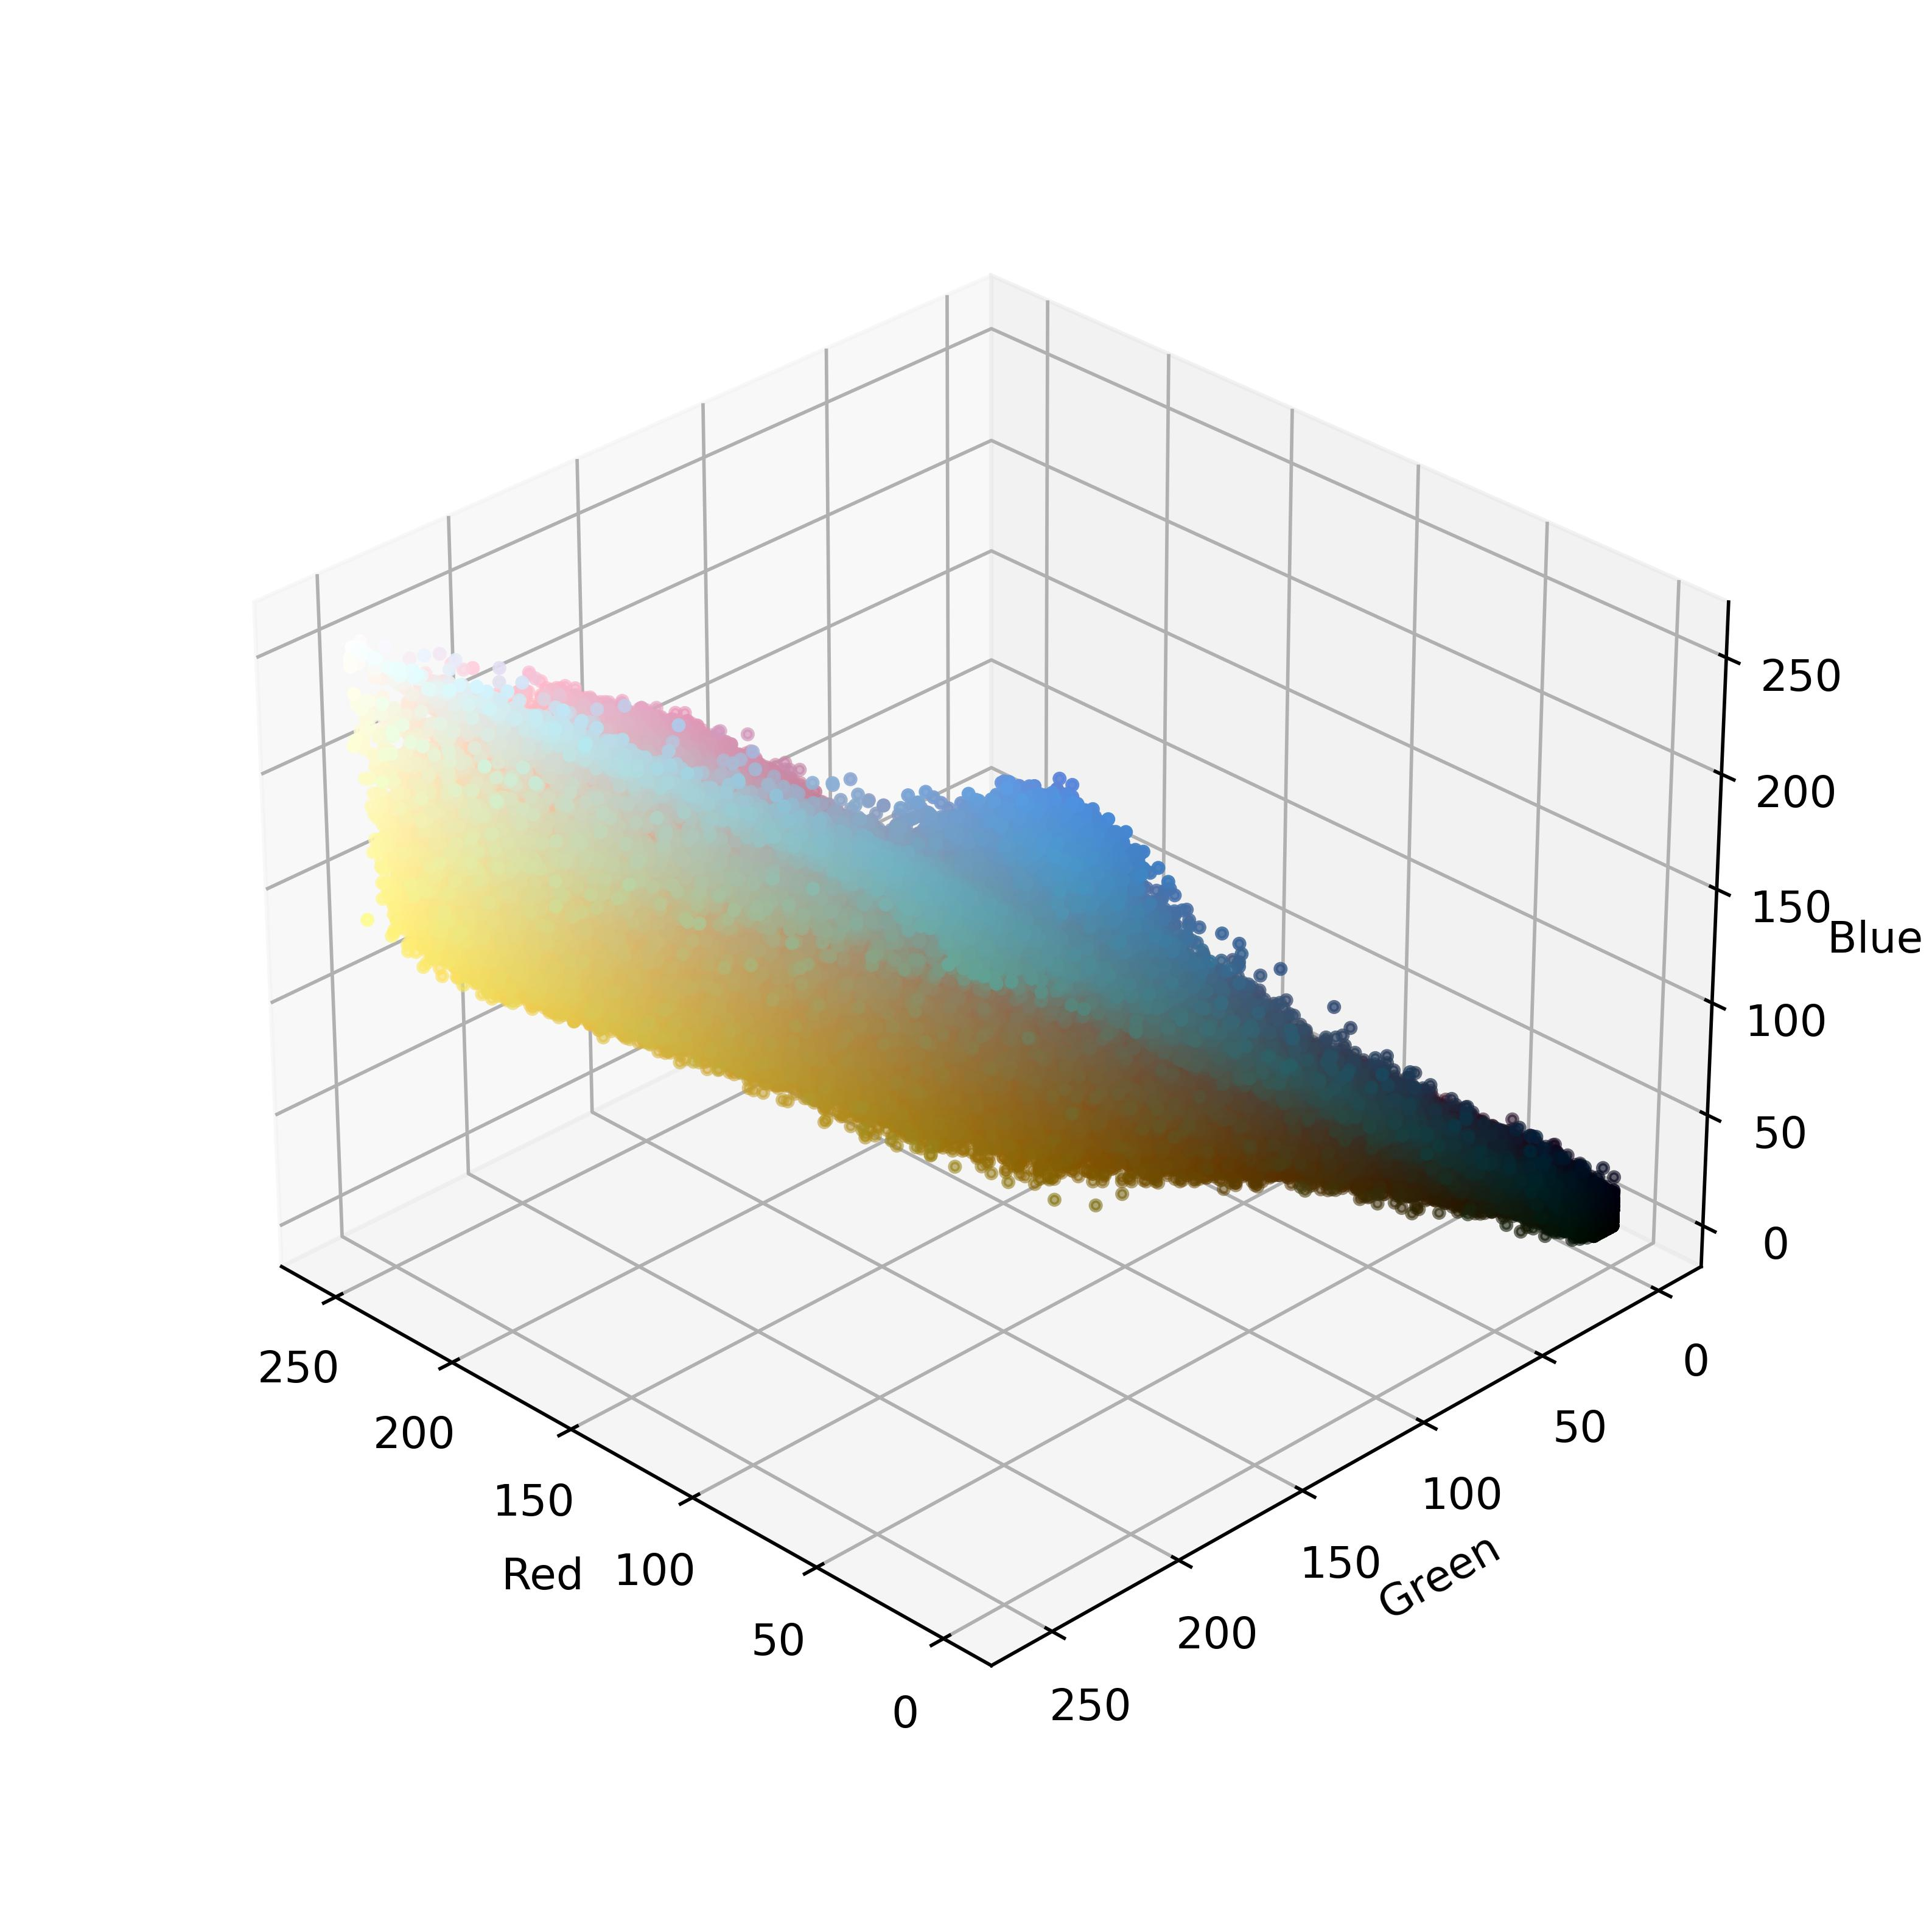
\includegraphics[width=\textwidth]{main_files/figure-latex/4_14_blue_marilyn_original_scatter.jpg}
    \caption{Blue Marilyn RGB Space - 30 \degree elevation, 135 \degree azimuth}
    \label{fig:4_14_blue_marilyn_original_scatter}
  \end{subfigure}
  \label{fig:blue_marilyn_original_scatter_1}
\end{figure}

\begin{figure}[ht]\ContinuedFloat
  \centering
  \begin{subfigure}{0.45\textwidth}
    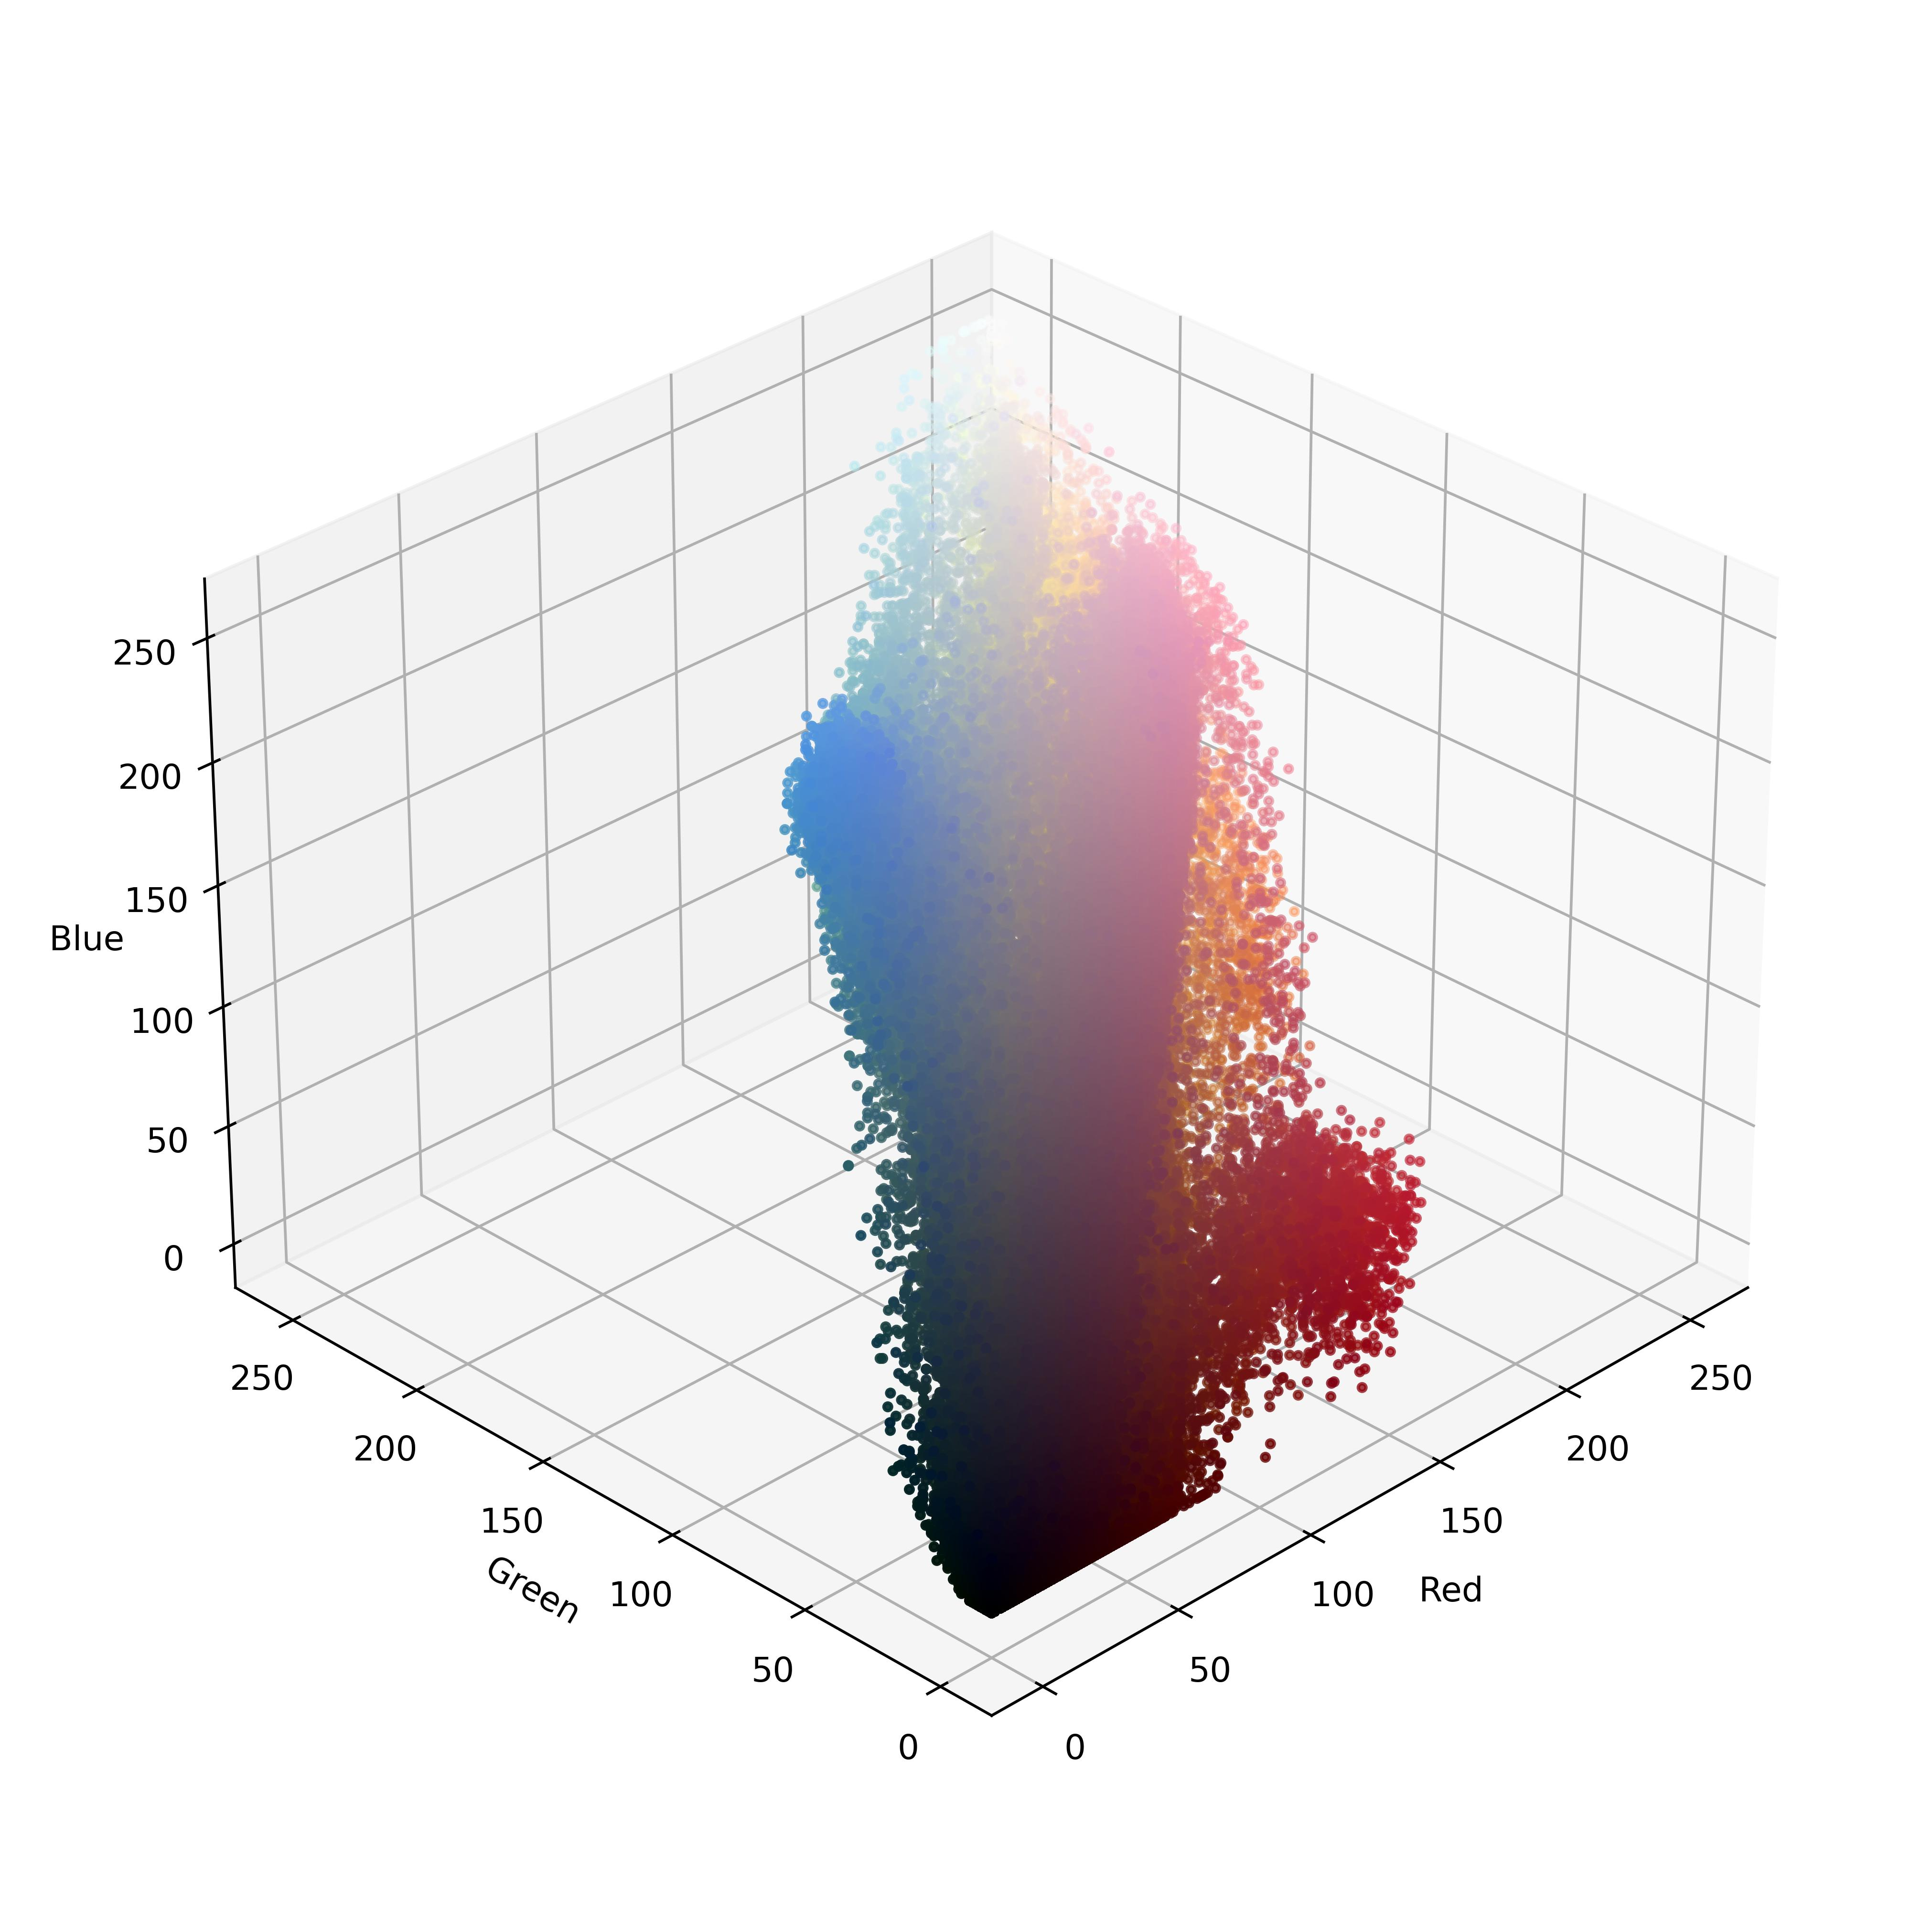
\includegraphics[width=\textwidth]{main_files/figure-latex/4_15_blue_marilyn_original_scatter.jpg}
    \caption{Blue Marilyn RGB Space - 30 \degree elevation, 225 \degree azimuth}
    \label{fig:4_15_blue_marilyn_original_scatter}
  \end{subfigure}
  \hfill
  \begin{subfigure}{0.45\textwidth}
    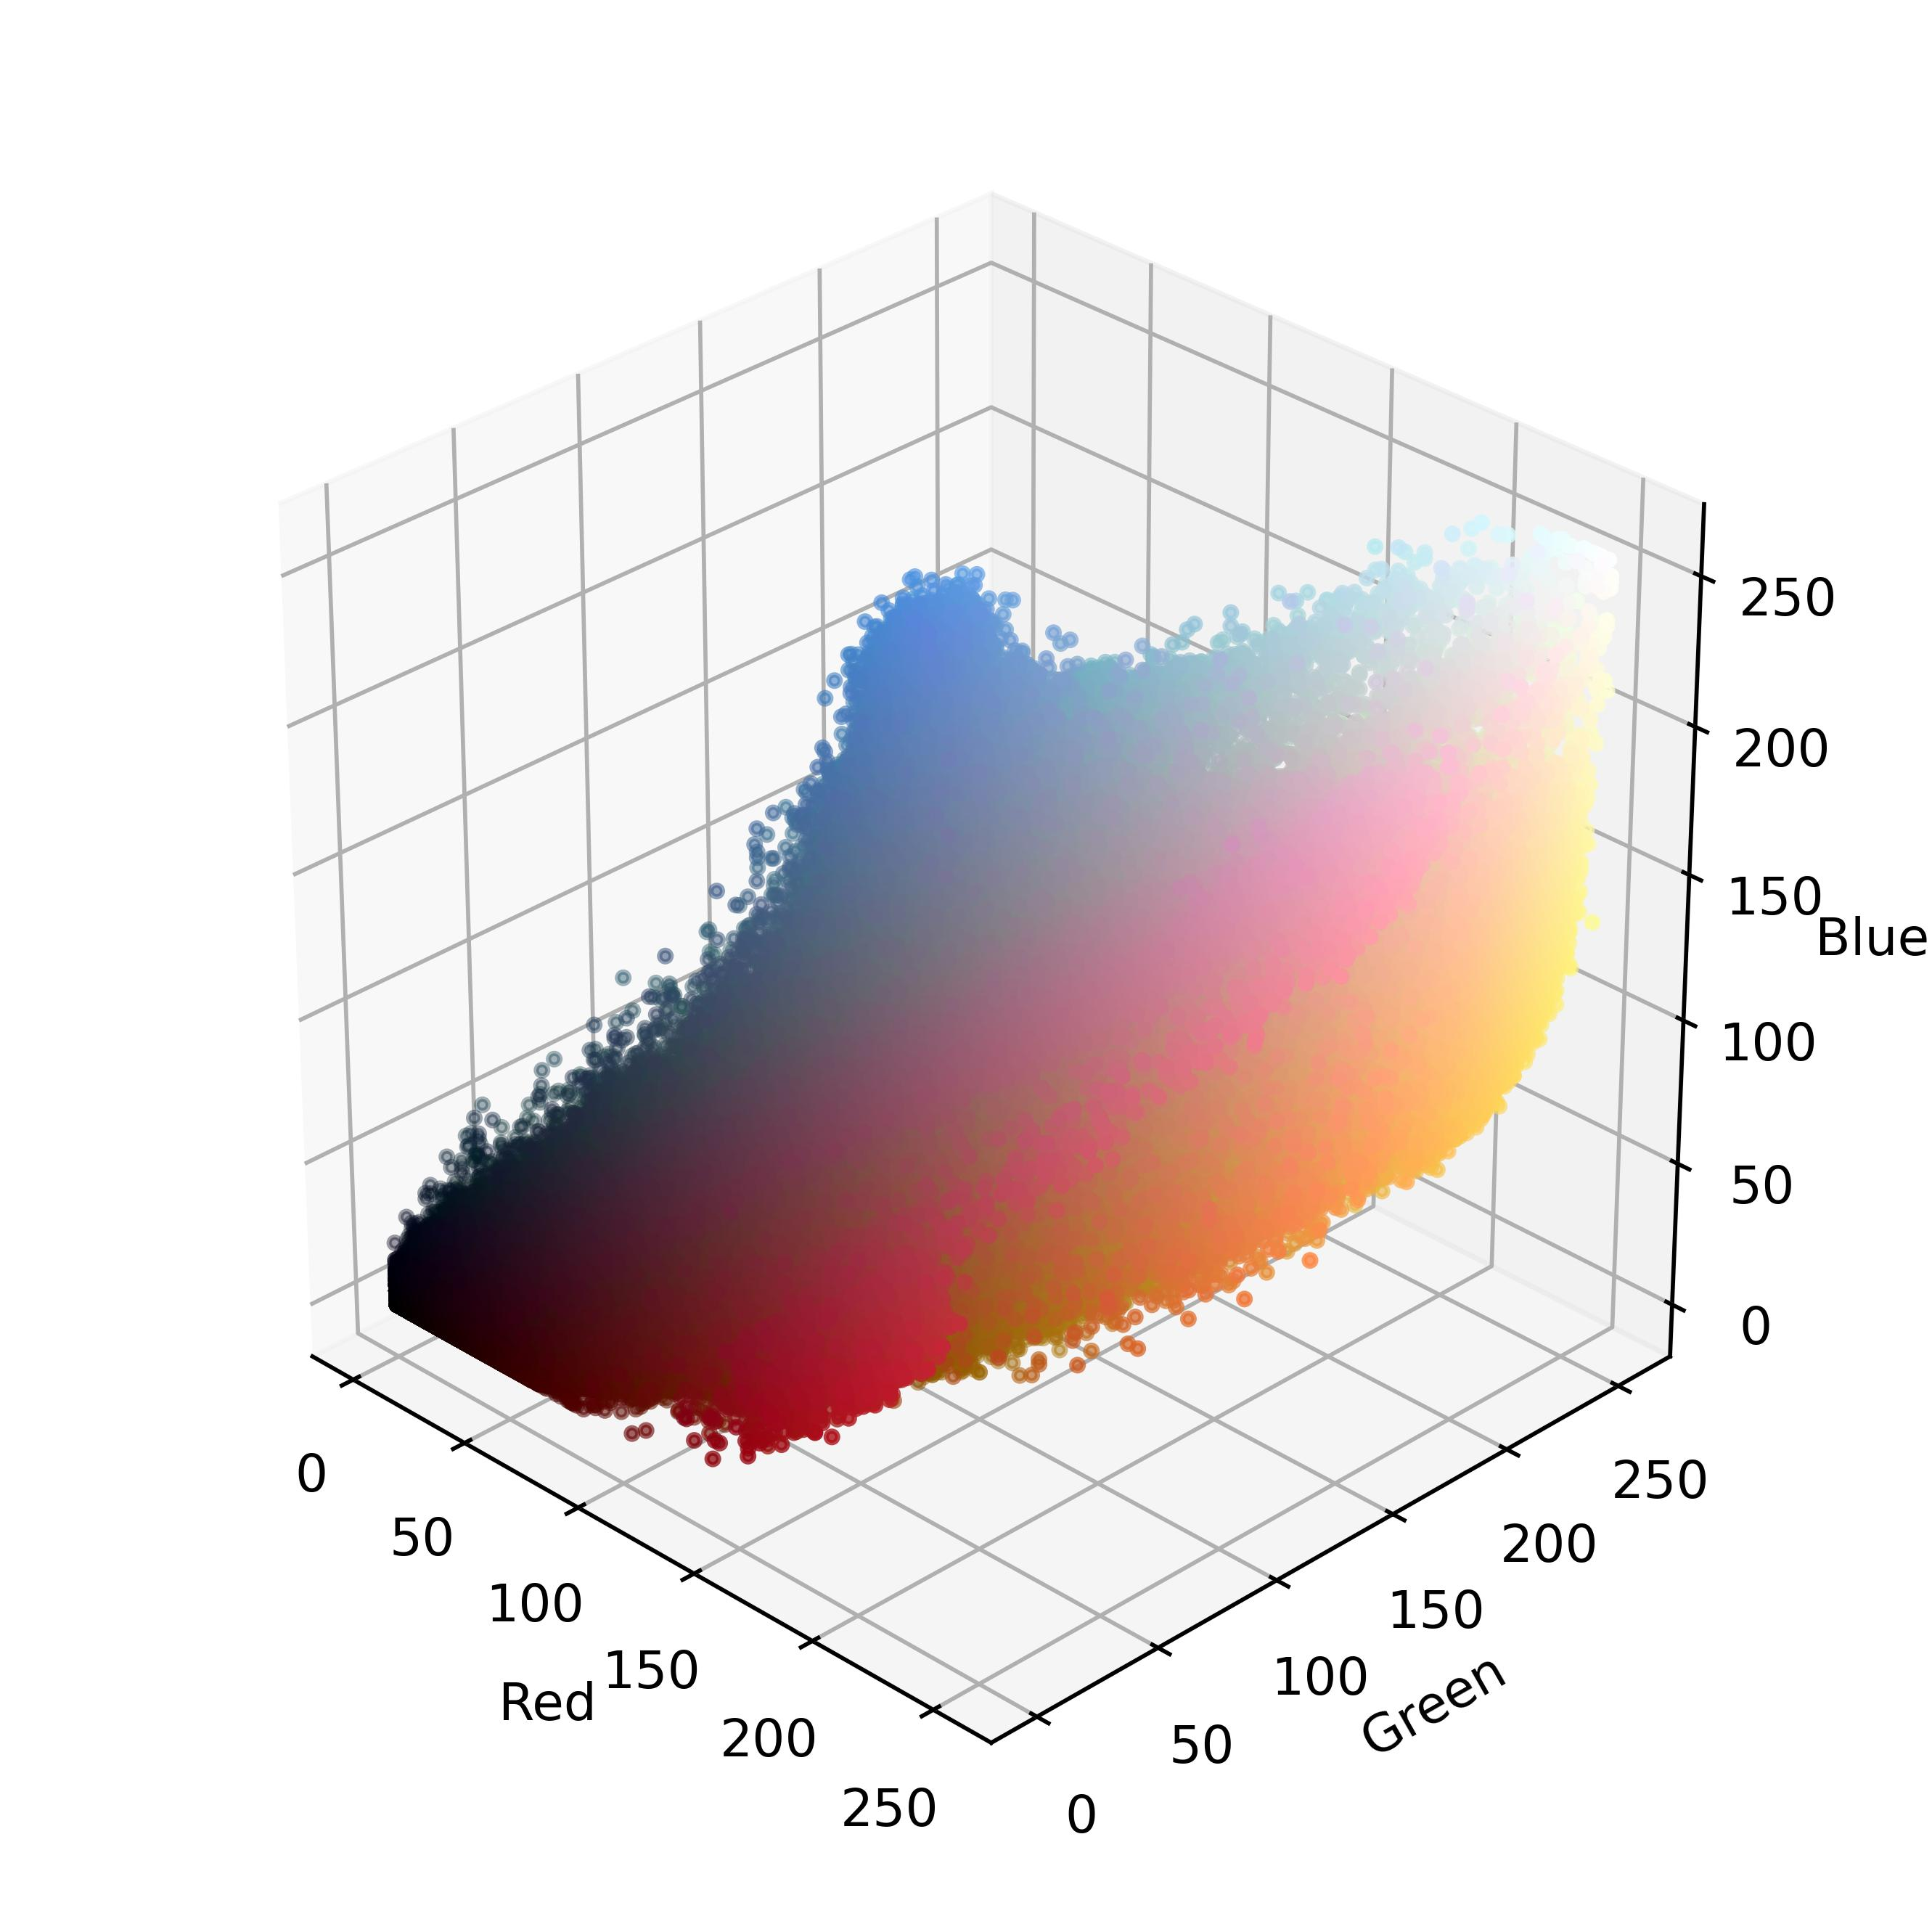
\includegraphics[width=\textwidth]{main_files/figure-latex/4_16_blue_marilyn_original_scatter.jpg}
    \caption{Blue Marilyn RGB Space - 30 \degree elevation, 315 \degree azimuth}
    \label{fig:4_16_blue_marilyn_original_scatter}
  \end{subfigure}
  \caption{The RGB space occupied by the pixels for the entire image of Blue Marilyn, showing different angles: (a) 30 \degree elevation, 45 \degree azimuth, (b) 30 \degree elevation, 135 \degree azimuth, (c) 30 \degree elevation, 225 \degree azimuth, (d) 30 \degree elevation, 315 \degree azimuth. These variations highlight the color distribution within the artwork.}
  \label{fig:blue_marilyn_original_scatter_2}
\end{figure}

Figure 7 displays the RGB space of ``Blue Marilyn'' from four different
angles.

In (a), the density of pixels shows a prominent mix of colors including
blue, yellow, pink, and red, which correspond to the background, hair,
face, and lips of the painting. The shape of the 3D scatter plot
indicates a broad, dispersed distribution of colors, reflecting the
varied color use throughout the image. Most pixels cluster in the blue
region, which is the dominant background color. The yellow pixels
representing Marilyn's hair extend prominently, indicating a significant
area covered by this hue.

In (b), the distribution of colors transitions from darker pixels on the
right side to brighter pixels on the left, highlighting a gradient. This
gradient is evident in the shading of Marilyn's facial features and
hair, adding depth to the portrait. The shape shows a clear separation
between dark and bright areas. The pink and red pixels, representing her
facial skin and lips, are more noticeable on the brighter side,
indicating the areas of the image where these colors are more
concentrated.

In (c), the plot shows the backside of (a), reaffirming the significant
presence of blue pixels. This view emphasizes the distribution of colors
in the facial highlights and hair, showing focused clustering of bright
colors where Warhol applied vivid hues. The shape indicates a dense
clustering of these bright pixels. The blue and yellow pixels are
prominently visible, showing the extensive use of these colors in the
background and hair.

In (d), the color distribution from dark to light is presented from a
different angle, allowing us to observe the spread of colors in areas
such as the hair and facial features. The shape reflects the backside of
(b), with darker pixels on the left and brighter pixels on the right.
The red pixels representing Marilyn's lips are more noticeable on the
brighter side, highlighting their vibrant color in the image. The shapes
in (b) through (d) reflect a similar elongated form, resembling a long
funnel, showing a clear gradient from dark to light colors.

Overall, these shapes and color distributions highlight how Warhol used
color to create depth and contrast in ``Blue Marilyn,'' emphasizing the
structured application of vivid and impactful colors to enhance the
visual experience. The different angles reveal the prominence of blue in
the background, yellow in the hair, pink in the facial skin, and red in
the lips, showcasing Warhol's strategic use of color to define the
features of Marilyn Monroe.

\begin{figure}[ht]
  \centering
  \begin{subfigure}{0.45\textwidth}
    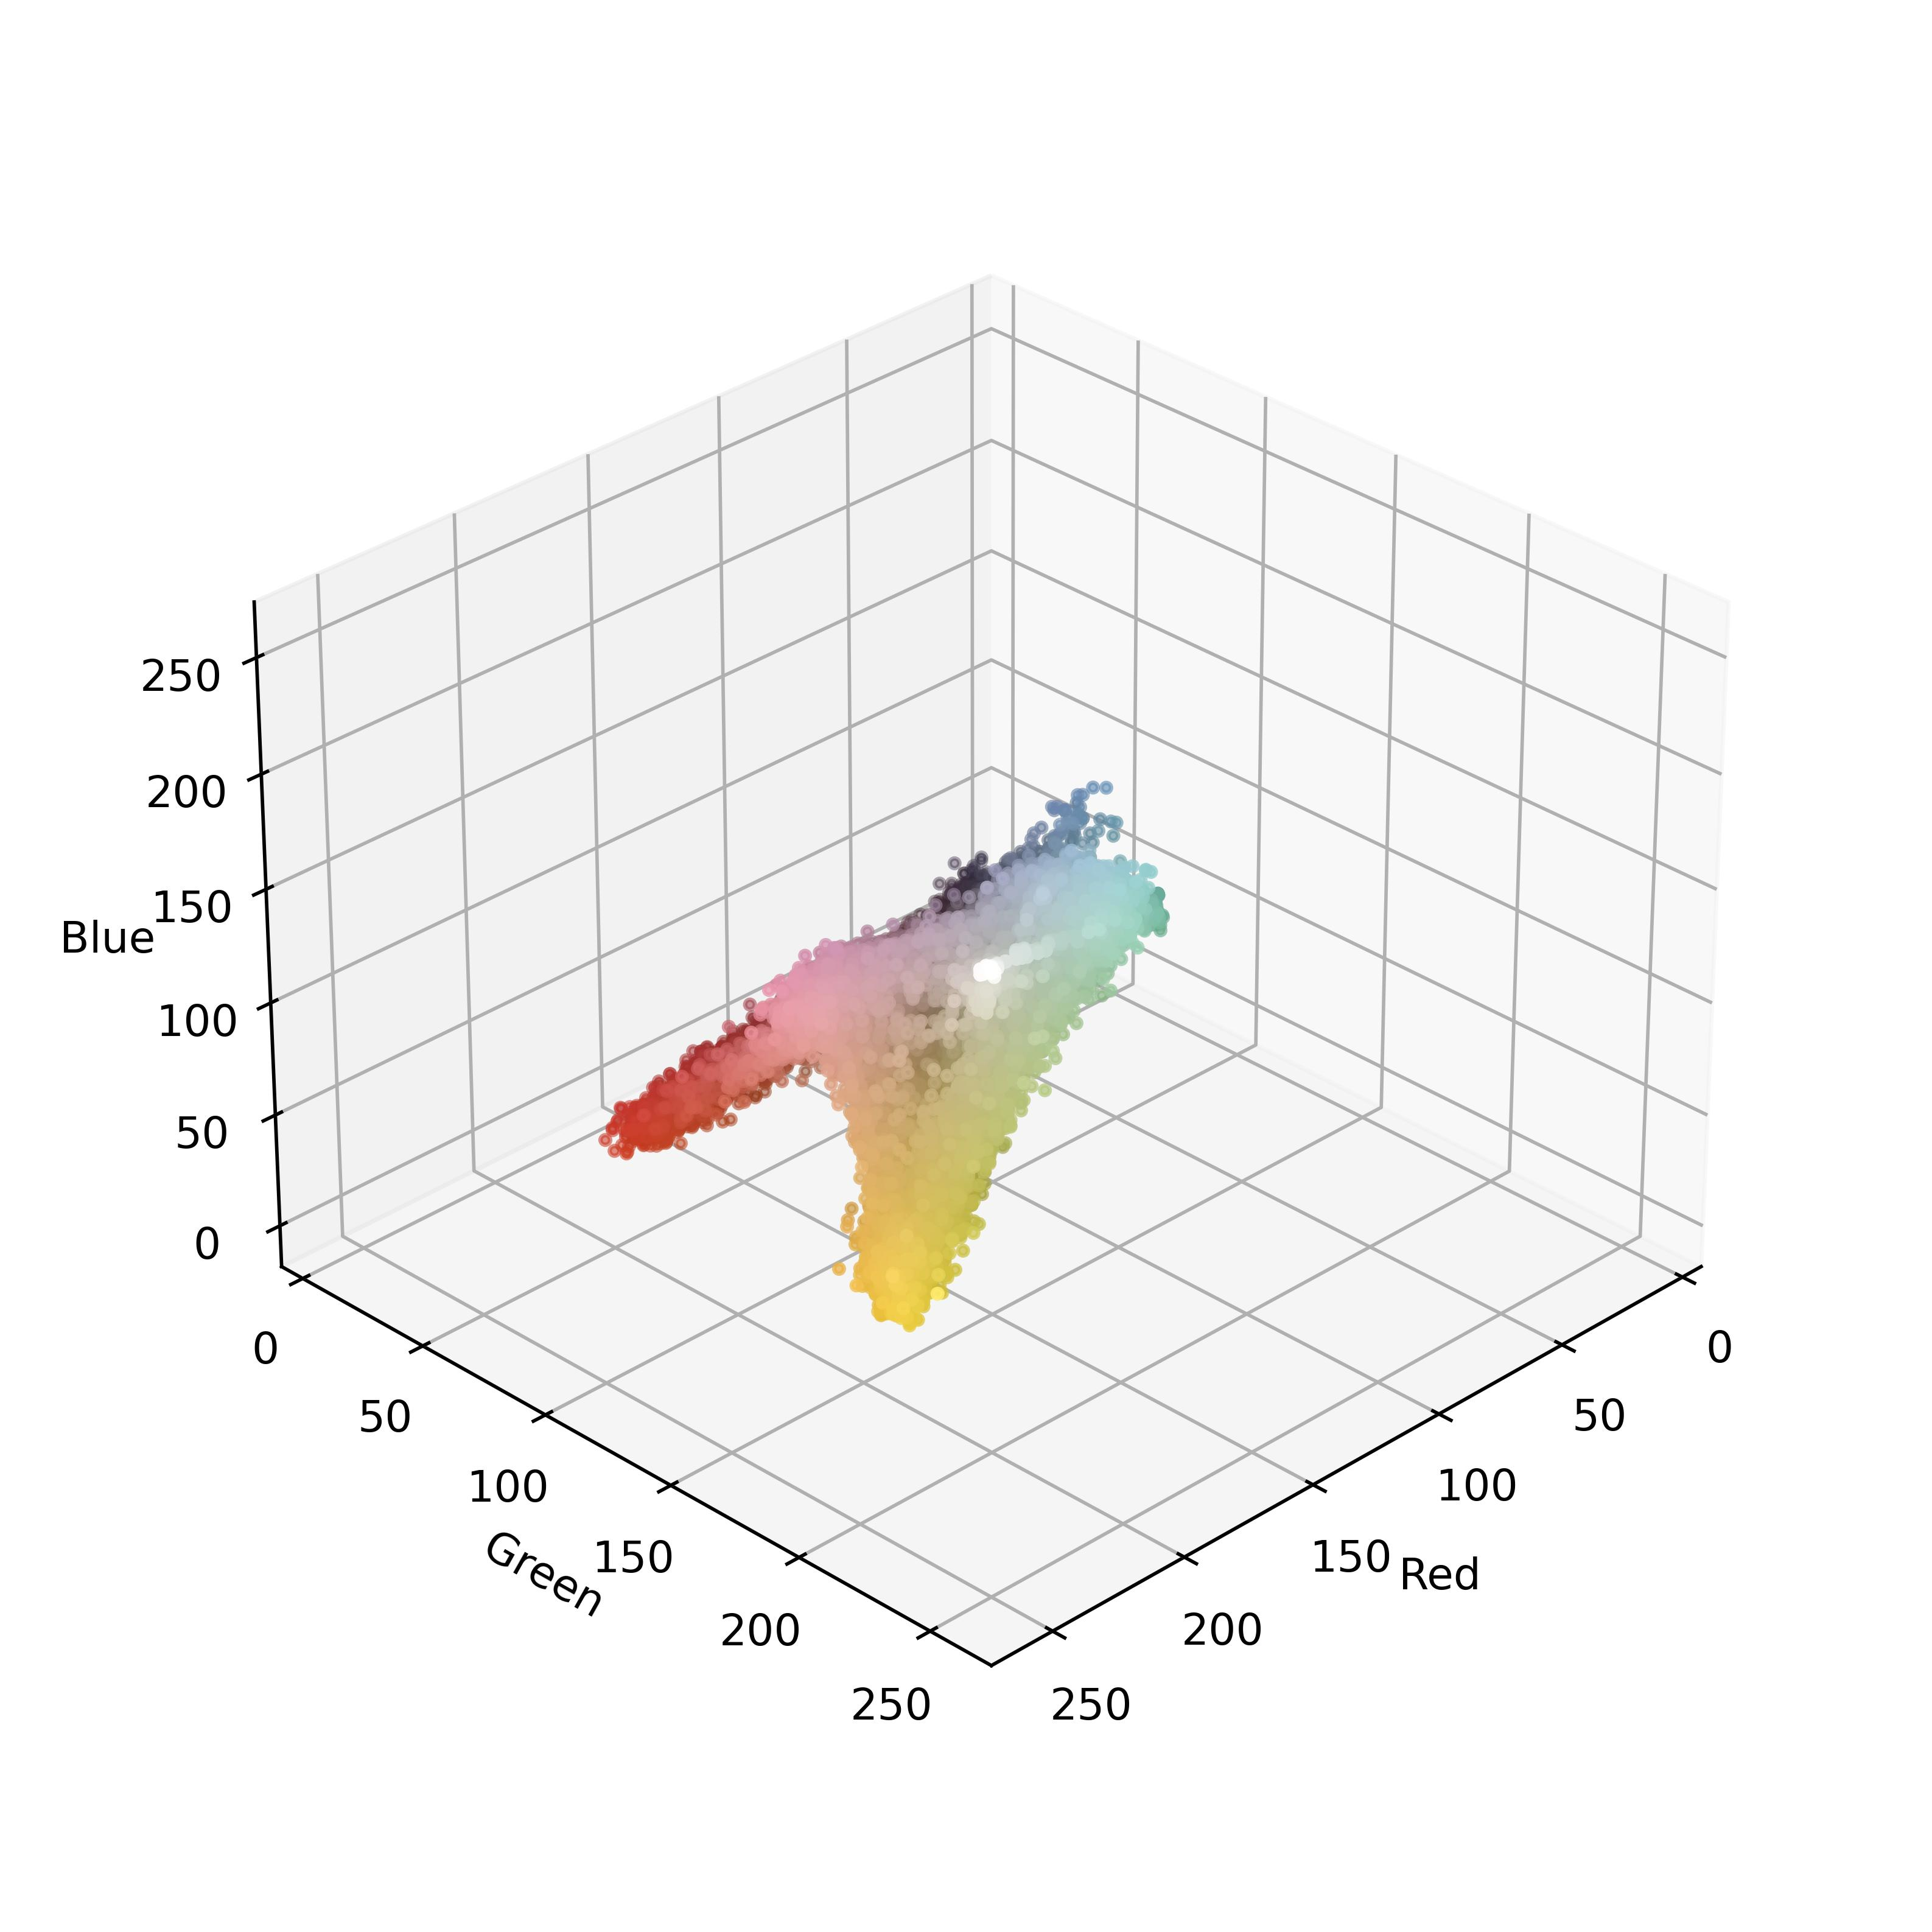
\includegraphics[width=\textwidth]{main_files/figure-latex/4_17_eggblue_marilyn_original_scatter.jpg}
    \caption{Eggblue Marilyn RGB Space - 30 \degree elevation, 45 \degree azimuth}
    \label{fig:4_17_eggblue_marilyn_original_scatter}
  \end{subfigure}
  \hfill
  \begin{subfigure}{0.45\textwidth}
    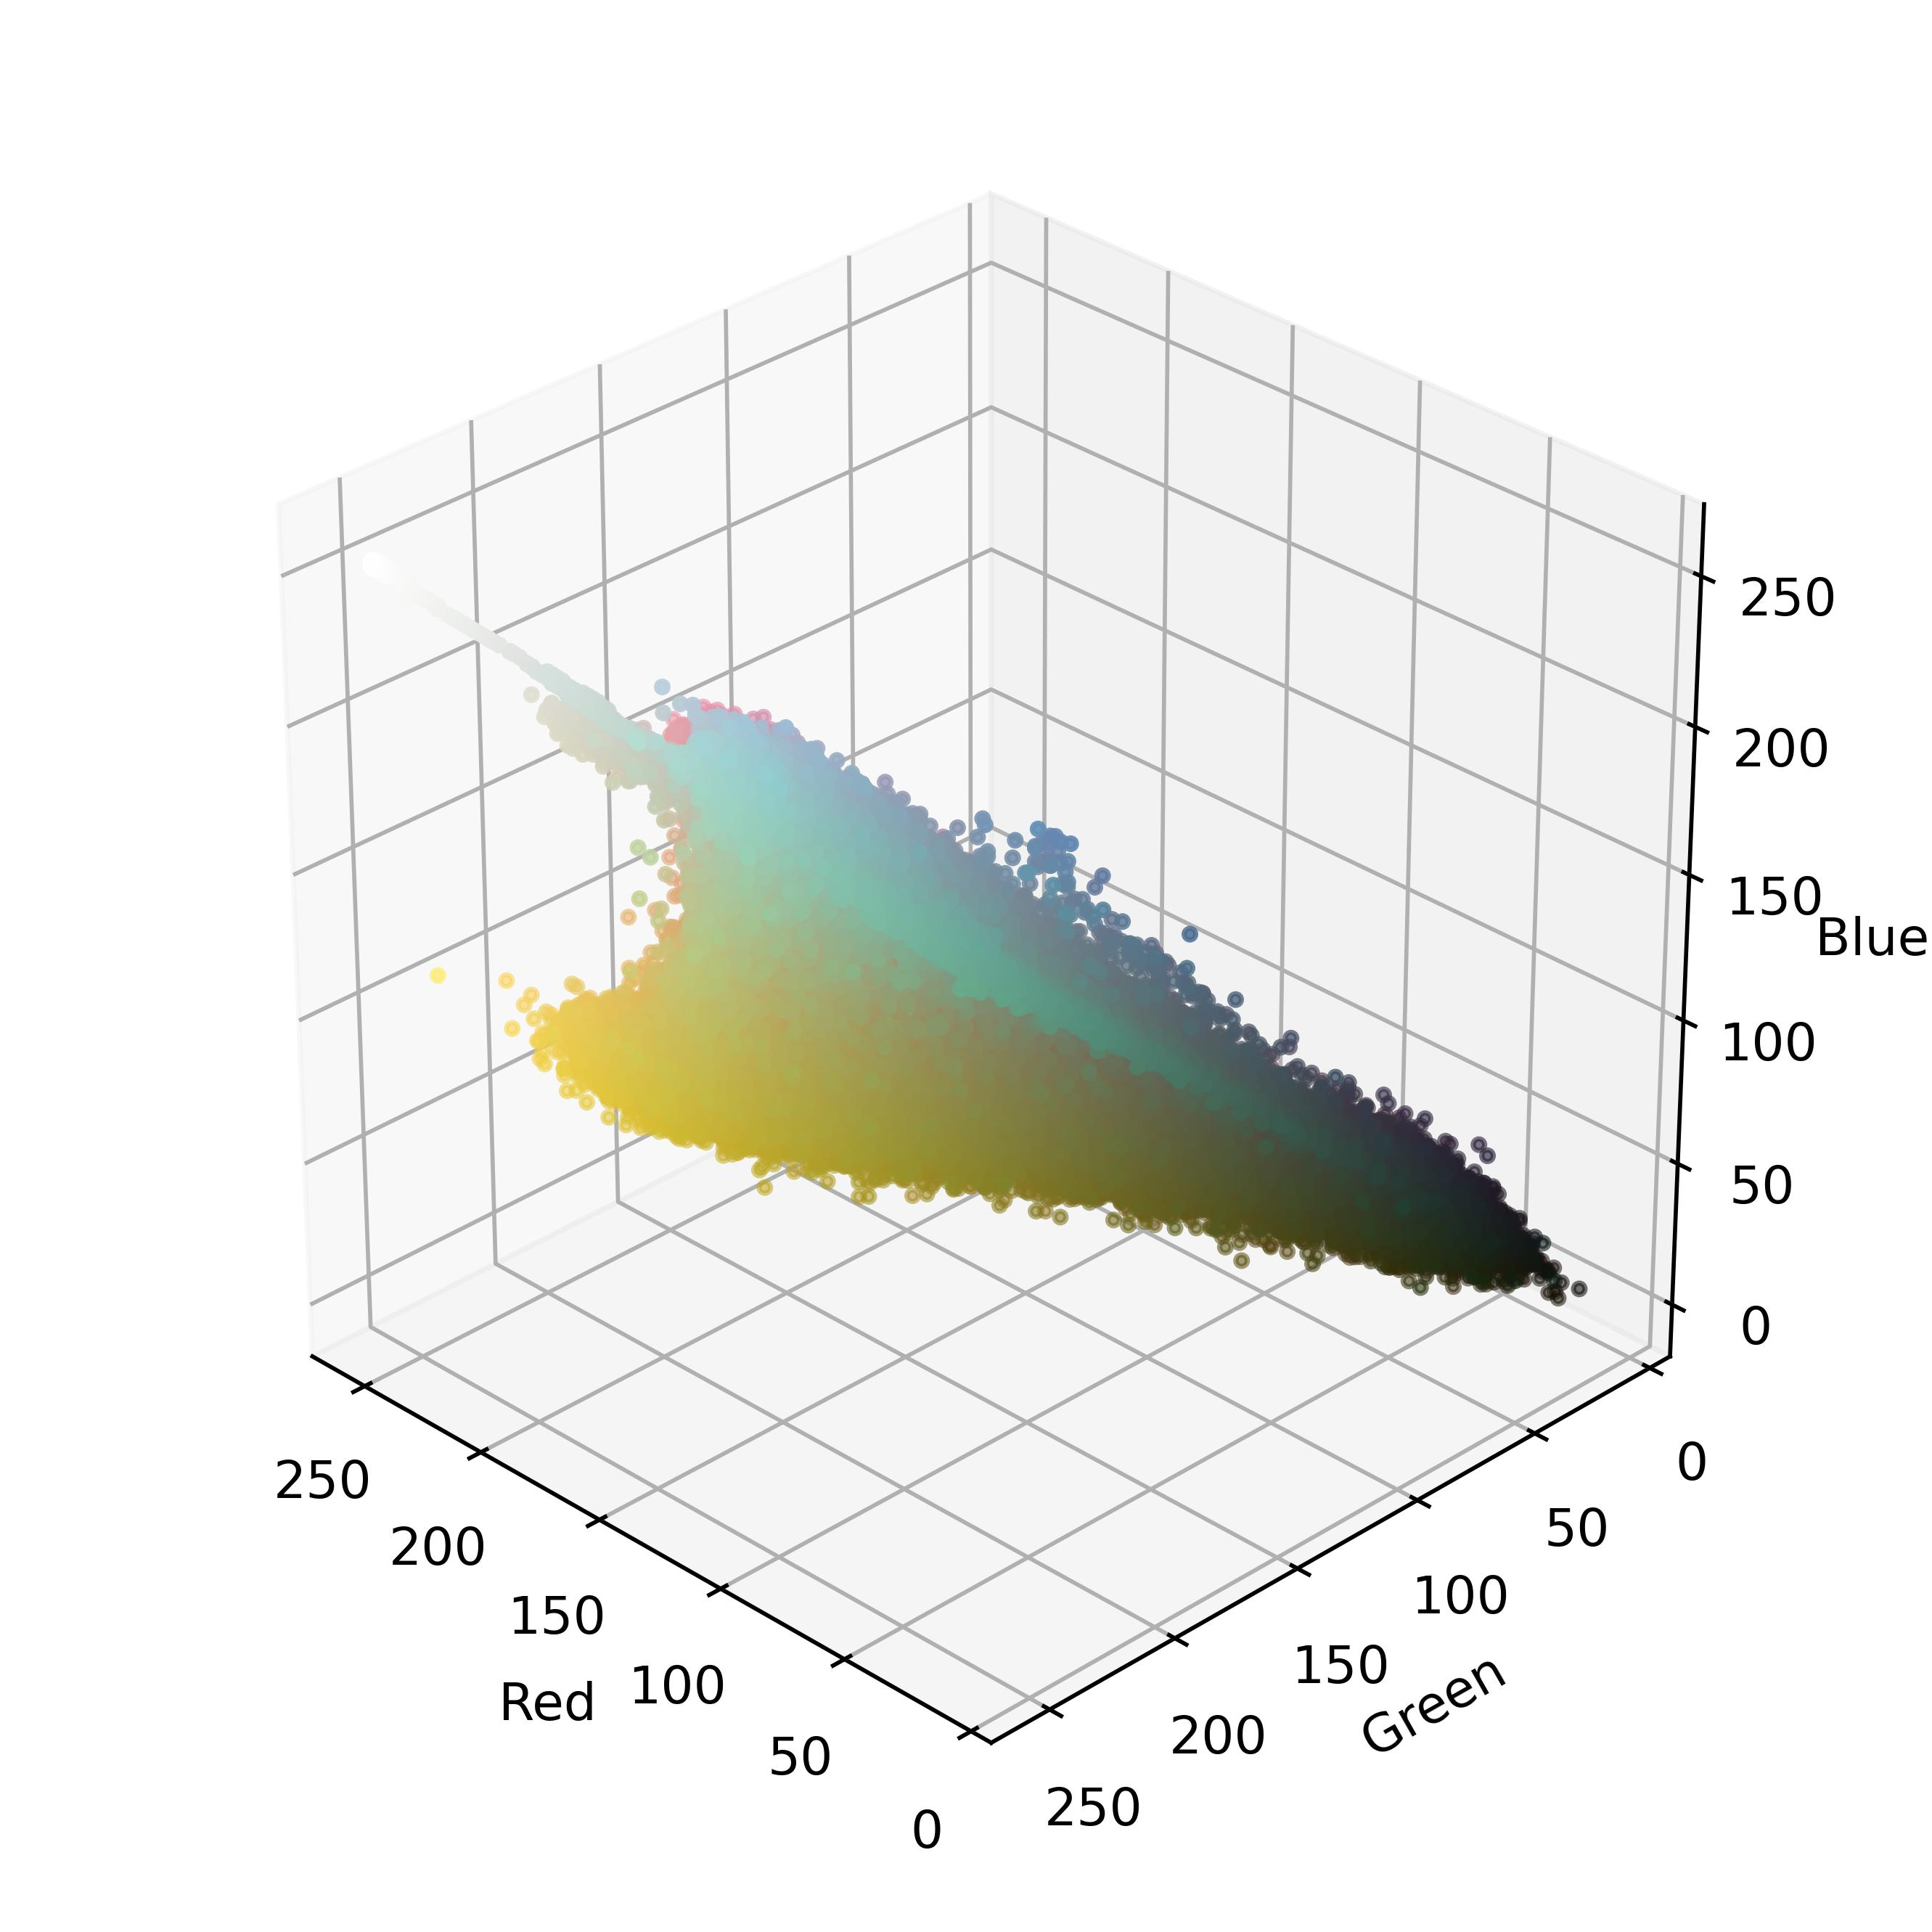
\includegraphics[width=\textwidth]{main_files/figure-latex/4_18_eggblue_marilyn_original_scatter.jpg}
    \caption{Eggblue Marilyn RGB Space - 30 \degree elevation, 135 \degree azimuth}
    \label{fig:4_18_eggblue_marilyn_original_scatter}
  \end{subfigure}
  \label{fig:eggblue_marilyn_original_scatter_1}
\end{figure}

\begin{figure}[ht]\ContinuedFloat
  \centering
  \begin{subfigure}{0.45\textwidth}
    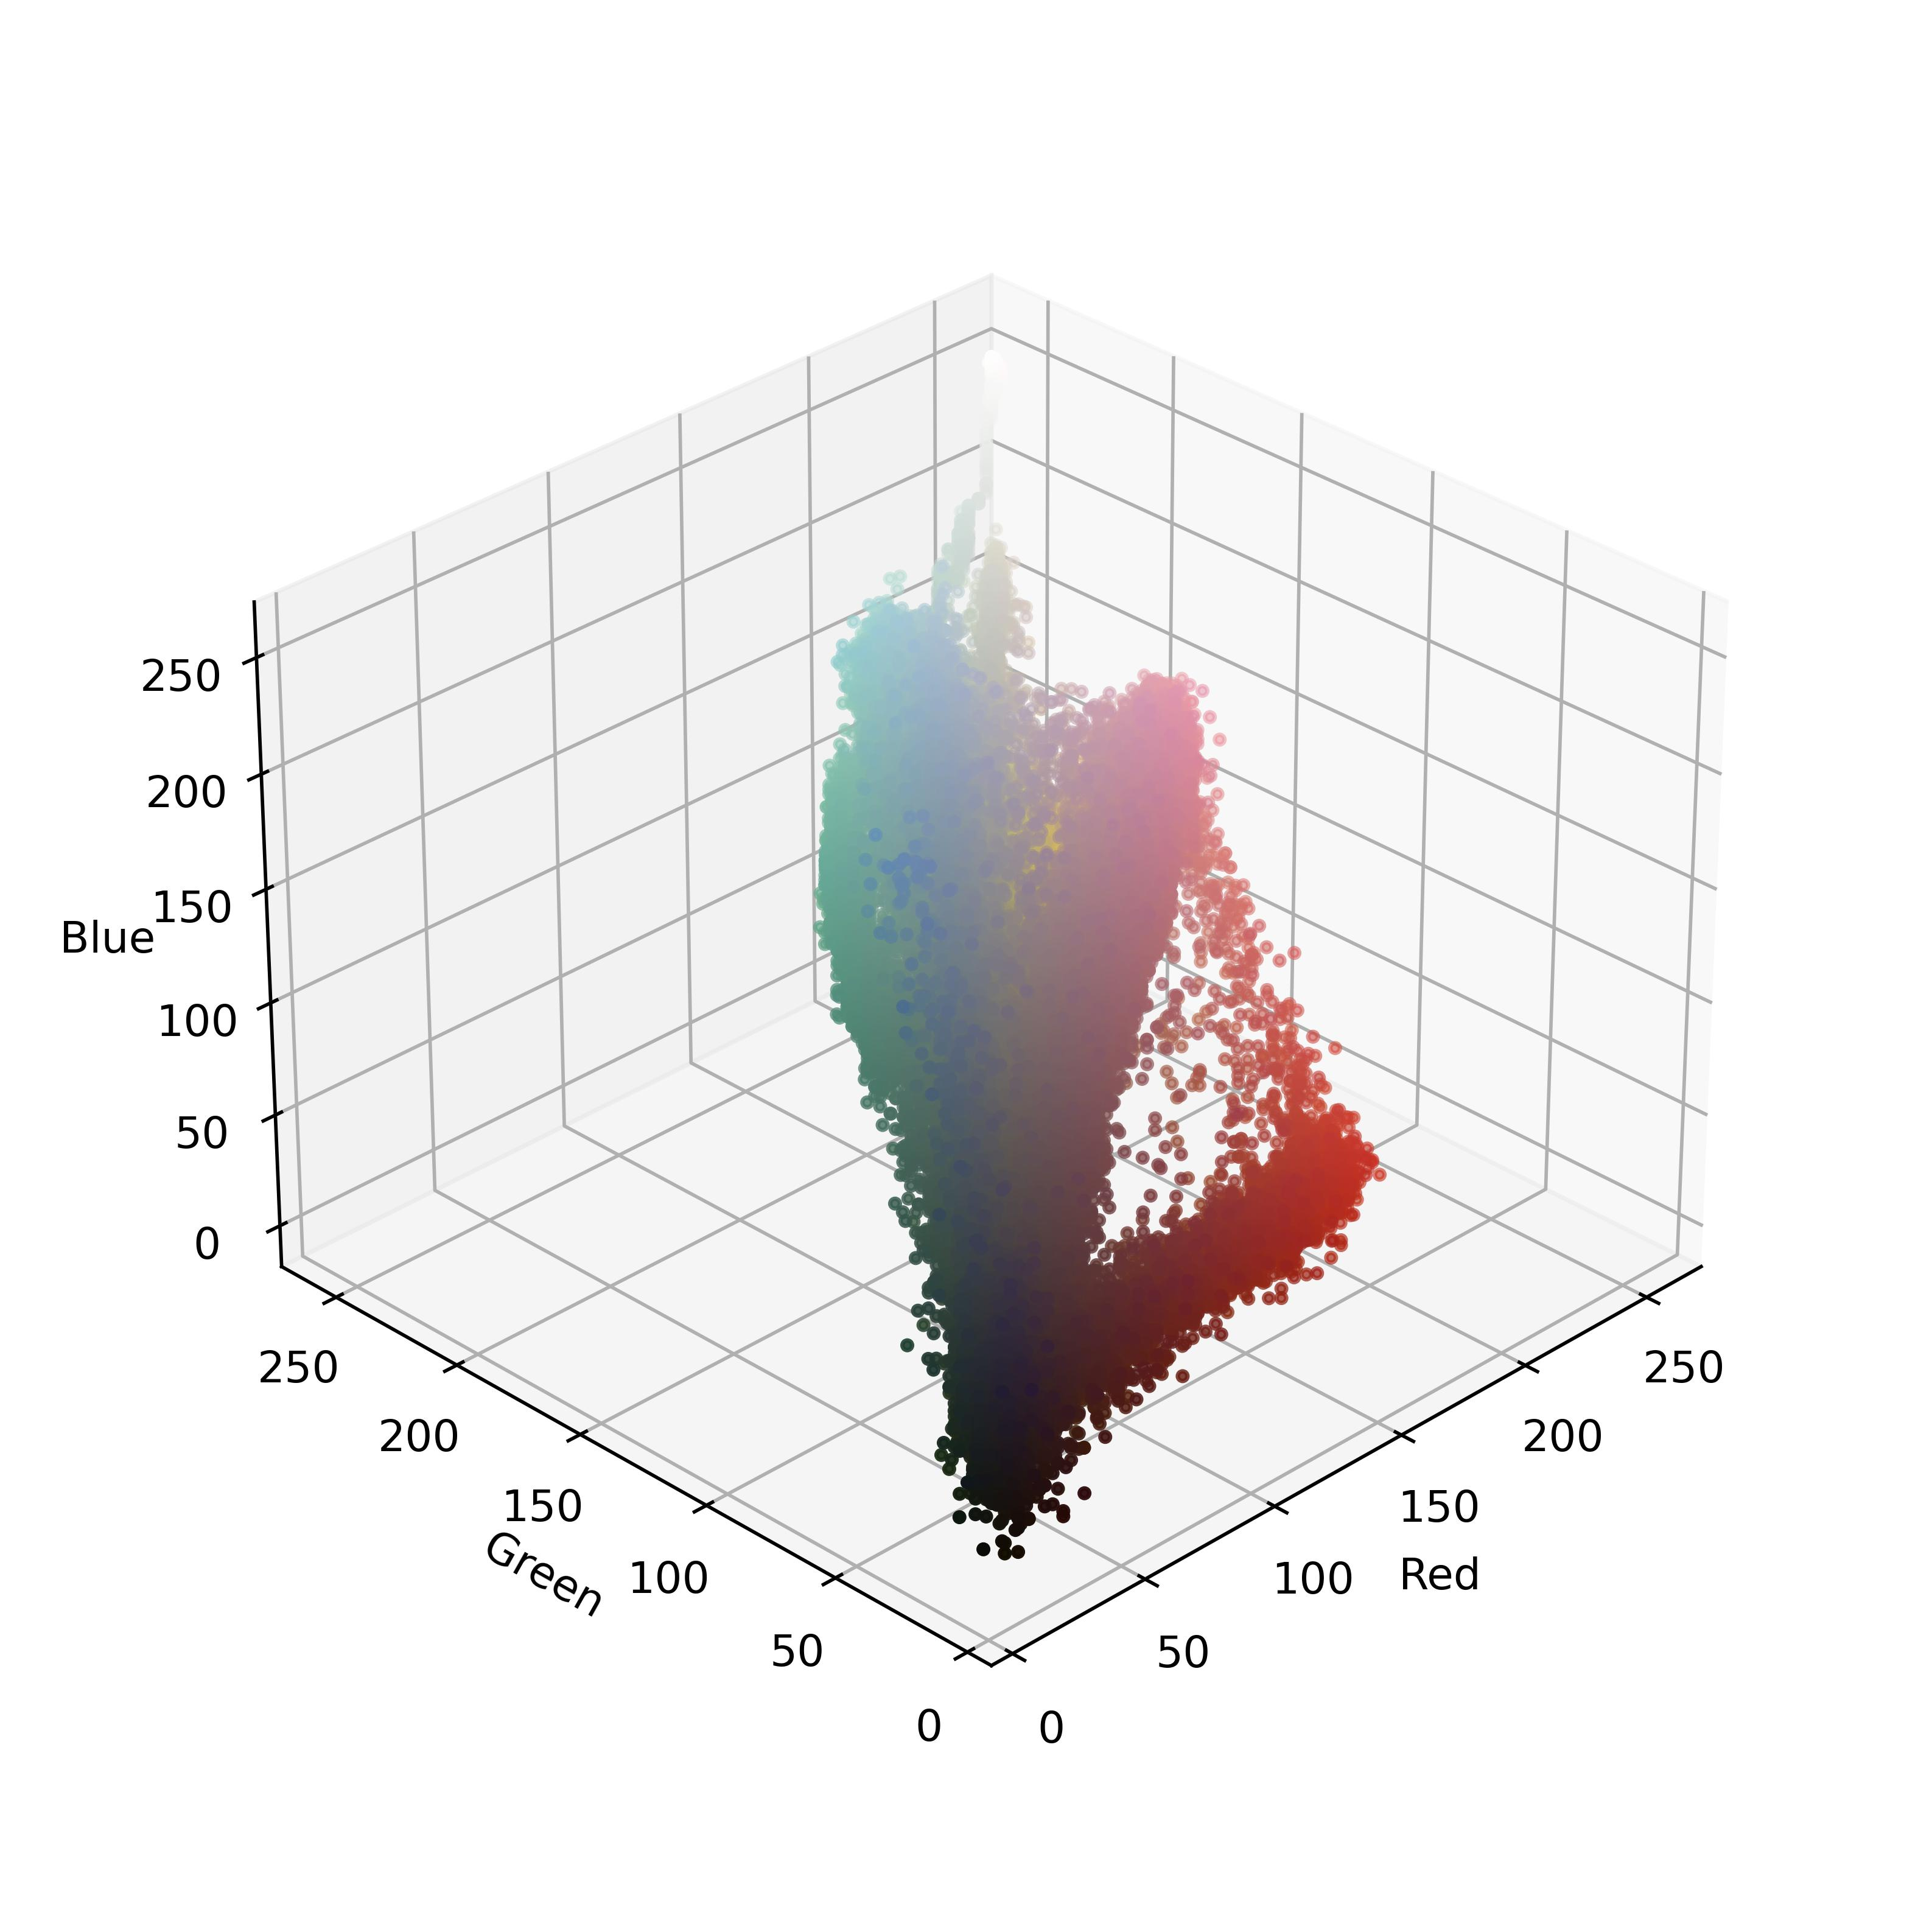
\includegraphics[width=\textwidth]{main_files/figure-latex/4_19_eggblue_marilyn_original_scatter.jpg}
    \caption{Eggblue Marilyn RGB Space - 30 \degree elevation, 225 \degree azimuth}
    \label{fig:4_19_eggblue_marilyn_original_scatter}
  \end{subfigure}
  \hfill
  \begin{subfigure}{0.45\textwidth}
    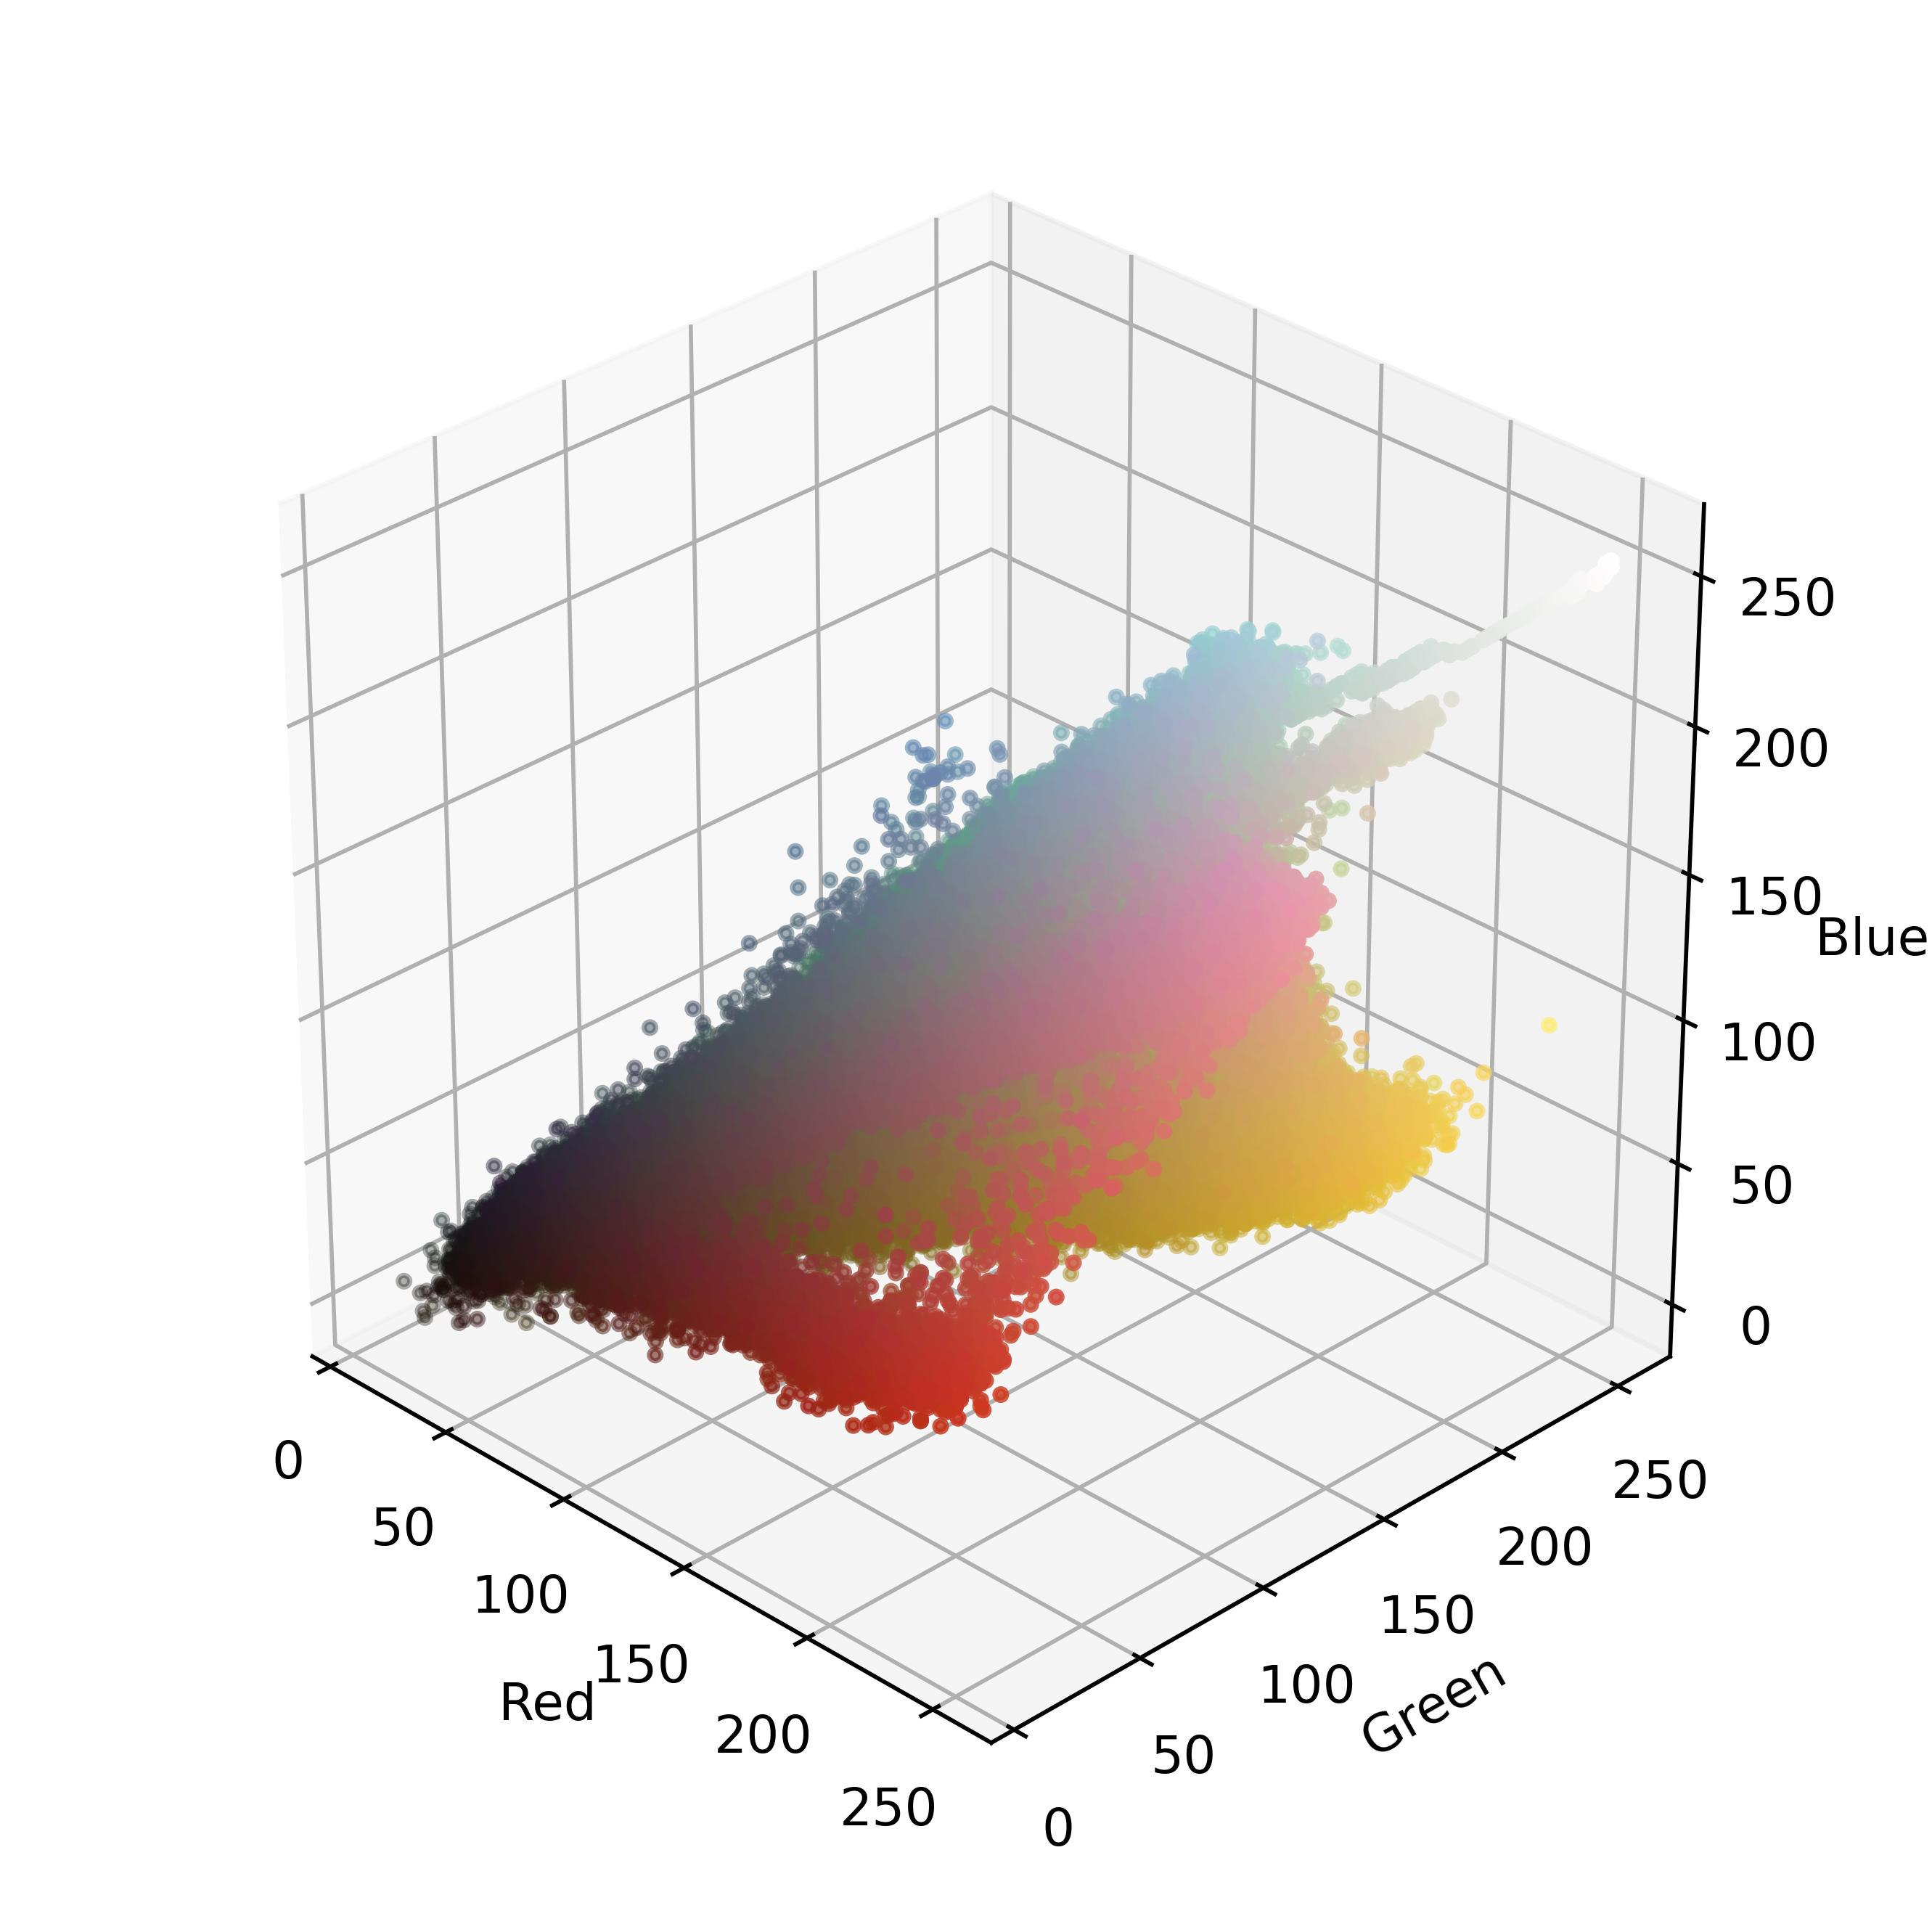
\includegraphics[width=\textwidth]{main_files/figure-latex/4_20_eggblue_marilyn_original_scatter.jpg}
    \caption{Eggblue Marilyn RGB Space - 30 \degree elevation, 315 \degree azimuth}
    \label{fig:4_20_eggblue_marilyn_original_scatter}
  \end{subfigure}
  \caption{The RGB space occupied by the pixels for the entire image of Eggblue Marilyn, showing different angles: (a) 30 \degree elevation, 45 \degree azimuth, (b) 30 \degree elevation, 135 \degree azimuth, (c) 30 \degree elevation, 225 \degree azimuth, (d) 30 \degree elevation, 315 \degree azimuth. These variations highlight the color distribution within the artwork.}
  \label{fig:eggblue_marilyn_original_scatter_2}
\end{figure}

Figure 8 displays the RGB space of ``Eggblue Marilyn'' from four
different angles.

In (a), the density of pixels shows a broad mix of colors including egg
blue, yellow, pink, and red, corresponding to the background, hair,
face, and lips of the painting. The shape of the 3D scatter plot
indicates a dispersed distribution of colors, reflecting the varied use
of hues throughout the image. Most pixels cluster in the egg blue
region, which is the dominant background color. Yellow pixels
representing Marilyn's hair extend prominently, indicating significant
coverage by this hue. At this angle, the egg blue background and yellow
hair colors are particularly noticeable.

In (b), the distribution of colors transitions from darker pixels on the
right side to brighter pixels on the left, highlighting a gradient. This
gradient illustrates the shading around Marilyn's facial features and
hair, adding depth to the portrait. The shape shows a clear separation
between dark and bright areas. The pink pixels representing her facial
skin and the red pixels of her lips are more noticeable on the brighter
side, indicating the areas of the image where these colors are more
concentrated. The egg blue and yellow pixels are also visible, but they
are less prominent from this angle.

In (c), the plot emphasizes the concentration of the brightest pixels,
showing specific groupings likely related to Marilyn's lips, eyes, and
other highlighted features. This view, showing the backside of (a),
reaffirms the significant presence of egg blue pixels. The yellow and
pink pixels are prominently visible, highlighting the extensive use of
these colors in the hair and facial features. The blue pixels in the eye
shadow are also noticeable, clustered with the bright pixels of the face
and hair.

In (d), the color distribution from dark to light is presented from a
different angle, allowing us to observe the spread of colors in areas
such as the hair and facial features. The shape reflects the backside of
(b), with darker pixels on the left and brighter pixels on the right.
The red pixels representing Marilyn's lips are more noticeable on the
brighter side, highlighting their vibrant color in the image. The yellow
pixels of her hair and the egg blue background pixels are more spread
out, showing a clear gradient from dark to light colors. The shapes in
(b) through (d) reflect a similar elongated form, resembling a long
funnel.

Overall, these shapes and color distributions highlight how Warhol used
color to create depth and contrast in ``Eggblue Marilyn.'' The different
angles reveal the prominence of egg blue in the background, yellow in
the hair, pink in the facial skin, red in the lips, and blue in the eye
shadow, showcasing Warhol's strategic use of color to define the
features of Marilyn Monroe. The detailed analysis of each angle provides
insights into how specific colors dominate different parts of the
painting and contribute to its overall visual impact.

\hypertarget{clustering-based-on-region-of-interest-roi}{%
\section{Clustering based on Region of Interest
(ROI)}\label{clustering-based-on-region-of-interest-roi}}

\hypertarget{repair-gunshot-of-image}{%
\section{Repair Gunshot of Image}\label{repair-gunshot-of-image}}

\hypertarget{disuccsion}{%
\section{Disuccsion}\label{disuccsion}}

\hypertarget{conclusion-and-future-work}{%
\section*{Conclusion and Future Work}\label{conclusion-and-future-work}}
\addcontentsline{toc}{section}{Conclusion and Future Work}

\hypertarget{refs}{}
\begin{CSLReferences}{1}{0}
\leavevmode\vadjust pre{\hypertarget{ref-arthur_2007_kmeans}{}}%
Arthur, David, and Sergei Vassilvitskii. 2007. {``K-Means++: The
Advantages of Careful Seeding.''} \emph{Symposium on Discrete
Algorithms}, January, 1027--35.
\url{https://doi.org/10.5555/1283383.1283494}.

\leavevmode\vadjust pre{\hypertarget{ref-christies_2022_andy}{}}%
Christie's. 2022. {``Andy Warhol's Marilyn: An Icon of Beauty.''}
Christie's.
\url{https://www.christies.com/en/stories/warhol-shot-marilyn-2629a4711b7e41f593e66bb2b33acd8b}.

\leavevmode\vadjust pre{\hypertarget{ref-masterworksfineartgallery_2019_andy}{}}%
Gallery, Masterworks Fine Art. 2019. {``Andy Warhol's "Shot
Marilyns".''} Masterworks Fine Art Gallery.
\url{https://news.masterworksfineart.com/2019/11/26/andy-warhols-shot-marilyns}.

\leavevmode\vadjust pre{\hypertarget{ref-ghighi_2022_andy}{}}%
Ghighi, Emma. 2022. {``Andy Warhol, the Shot Marilyns, and His Early
Silkscreens.''} Revolver Gallery.
\url{https://revolverwarholgallery.com/andy-warhol-the-shot-marilyns-and-his-early-silkscreens/}.

\leavevmode\vadjust pre{\hypertarget{ref-lanchner_2008_andy}{}}%
Lanchner, Carolyn, and Andy Warhol. 2008. \emph{Andy Warhol}. The Museum
of Modern Art, New York.

\leavevmode\vadjust pre{\hypertarget{ref-shannon_1948_a}{}}%
Shannon, C. E. 1948. {``A Mathematical Theory of Communication.''}
\emph{Bell System Technical Journal} 27: 379--423.

\leavevmode\vadjust pre{\hypertarget{ref-vankin_2022_sold}{}}%
Vankin, Deborah. 2022. Los Angeles Times.
\url{https://www.latimes.com/entertainment-arts/story/2022-05-09/andy-warhols-shot-sage-blue-marilyn-sets-new-auction-record}.

\end{CSLReferences}

\bibliographystyle{unsrt}
\bibliography{references.bib}


\end{document}
